% Volatility Forecasting Project - MATH 287C Spring 2018
% Nishant D. Gurnani

%%%%%%%%%%%%%%%%%%%%%%%%%%%%%%%%%%%%%%%%%%%%%%%%%%%%%%%%%%%%%%%%%%%%%%%%%%%%%
\documentclass{beamer}
\mode<presentation> {
\usetheme{default}
\setbeamertemplate{footline}[page number]
\setbeamertemplate{section in toc}[sections numbered]
\setbeamercovered{invisible}
% To remove the navigation symbols from the bottom of slides%
\setbeamertemplate{navigation symbols}{} 
}

\usepackage{mathtools}
\DeclarePairedDelimiter{\ceil}{\lceil}{\rceil}


\newcommand{\id}{\mathrm{id}}
\newcommand{\K}{\mathrm{KL}}
\newcommand{\kl}{\mathrm{kl}}
\newcommand{\bp}{\boldsymbol{p}}
\renewcommand{\phi}{\varphi}
\renewcommand{\a}{\alpha}

\renewcommand{\P}{\mathbb{P}}
\newcommand{\E}{\mathbb{E}}
\newcommand{\N}{\mathbb{N}}
\newcommand{\R}{\mathbb{R}}
\newcommand{\Q}{\mathbb{Q}}
\newcommand{\KL}{\mathrm{KL}}
\newcommand{\LG}{\overline{\log}(d)}
\newcommand{\LGG}{\overline{\log}(M K)}
\newcommand{\ocP}{\overline{\mathcal{P}}}

\newcommand{\cO}{\mathcal{O}}
\newcommand{\cZ}{\mathcal{Z}}
\newcommand{\cA}{\mathcal{A}}
\newcommand{\cB}{\mathcal{B}}
\newcommand{\cN}{\mathcal{N}}
\newcommand{\cM}{\mathcal{M}}
\newcommand{\cF}{\mathcal{F}}
\newcommand{\cL}{\mathcal{L}}
\newcommand{\cX}{\mathcal{X}}
\newcommand{\cI}{\mathcal{I}}
\newcommand{\cJ}{\mathcal{J}}
\newcommand{\cY}{\mathcal{Y}}
\newcommand{\cH}{\mathcal{H}}
\newcommand{\cP}{\mathcal{P}}
\newcommand{\cT}{\mathcal{T}}
\newcommand{\cC}{\mathcal{C}}
\newcommand{\cS}{\mathcal{S}}
\newcommand{\cE}{\mathcal{E}}
\newcommand{\cK}{\mathcal{K}}
\newcommand{\cD}{\mathcal{D}}

\newcommand{\oD}{\overline{\mathcal{D}}}
\newcommand{\oR}{\overline{R}}

\def\ds1{\mathds{1}}
\renewcommand{\epsilon}{\varepsilon}

\newcommand{\wh}{\widehat}
\newcommand{\argmax}{\mathop{\mathrm{argmax}}}
\newcommand{\argmin}{\mathop{\mathrm{argmin}}}
\renewcommand{\mod}[2]{[#1 \,\, \mathrm{mod} \,\, #2]}
\newcommand{\todo}{{\bf TO DO } }

\renewcommand{\tilde}{\widetilde}

%Cadres d'algorithmes
\newlength{\minipagewidth}
\setlength{\minipagewidth}{\columnwidth}
\setlength{\fboxsep}{3mm}
\addtolength{\minipagewidth}{-\fboxrule}
\addtolength{\minipagewidth}{-\fboxrule}
\addtolength{\minipagewidth}{-\fboxsep}
\addtolength{\minipagewidth}{-\fboxsep}
\newcommand{\bookbox}[1]{\small
\par\medskip\noindent
\framebox[\columnwidth]{
\begin{minipage}{\minipagewidth} {#1} \end{minipage} } \par\medskip }

%%
%

\newcommand{\Ber}{\mathop{\mathrm{Ber}}}

\newcommand{\beq}{\begin{equation}}
\newcommand{\eeq}{\end{equation}}

\newcommand{\beqa}{\begin{eqnarray}}
\newcommand{\eeqa}{\end{eqnarray}}

\newcommand{\beqan}{\begin{eqnarray*}}
\newcommand{\eeqan}{\end{eqnarray*}}

\def\ba#1\ea{\begin{align*}#1\end{align*}} %\ba = \begin{algin*}, \ea = \end{align*}
\def\banum#1\eanum{\begin{align}#1\end{align}} %\banum = \begin{algin}, \eanum

%\newcommand{\qed}{\hfill\BlackBox}
\newcommand{\charfct}{\ds1} %
\newcommand{\Fcal}{\mathcal{F}}
\newcommand{\Xcal}{\mathcal{X}}
\newcommand{\Hcal}{\mathcal{H}}
\newcommand{\Gcal}{\mathcal{G}}
\newcommand{\Nat}{\mathbb{N}}


\newcounter{saveenumi}
\newcommand{\seti}{\setcounter{saveenumi}{\value{enumi}}}
\newcommand{\conti}{\setcounter{enumi}{\value{saveenumi}}}

\usepackage{natbib} % for citations
\usepackage{graphicx}
\usepackage{subfig}
\usepackage{bm} 

\newcounter{saveenumi}
\newcommand{\seti}{\setcounter{saveenumi}{\value{enumi}}}
\newcommand{\conti}{\setcounter{enumi}{\value{saveenumi}}}

\resetcounteronoverlays{saveenumi}

%\setbeamerfont{institute}{size=\medium}
\setbeamerfont{date}{size=\tiny}
%%%%%%%%%%%%%%%%%%%%%%%%%%%%%%%%%%%%%%%%%%%%%%%%%%%%%%%%%%%%%%%%%%%%%%%%%%%%%

\title[]{A Practical Look at Volatility in Financial Time Series}
\author{MATH 287C - Advanced Time Series Analysis \\ Nishant Gurnani}
\date{June 4th, 2018}

\begin{document}

% Title Slide
\begin{frame}
\titlepage
\end{frame}


% TOC SLIDE
\begin{frame}
\frametitle{Outline}
\tableofcontents[]
\end{frame}

% SECTION 1
\section{What is Volatility?}

\begin{frame}
\frametitle{Outline}
\tableofcontents[currentsection]
\end{frame}

\begin{frame}
\frametitle{What is Volatility?}
\begin{itemize}
\item{Volatility is a measure of price variability over some period of time}
\item{Typically described by the standard deviation $\sigma$ of the return series $\{X_t\}$}
\item{Volatility is peculiar in that we know it exists, but in some sense we can't really measure it}
\item{Bachelier (1900) showed that $\{X_t\} \sim$ iid. $N(0,1)$, but this is only good for a first order approximation}
\end{itemize}
\end{frame}

\begin{frame}
\frametitle{Naive Measure - Realized Volatility}
%Realized volatility, also called historical volatility, is the standard deviation of a set of previous returns
\begin{figure}[h!]
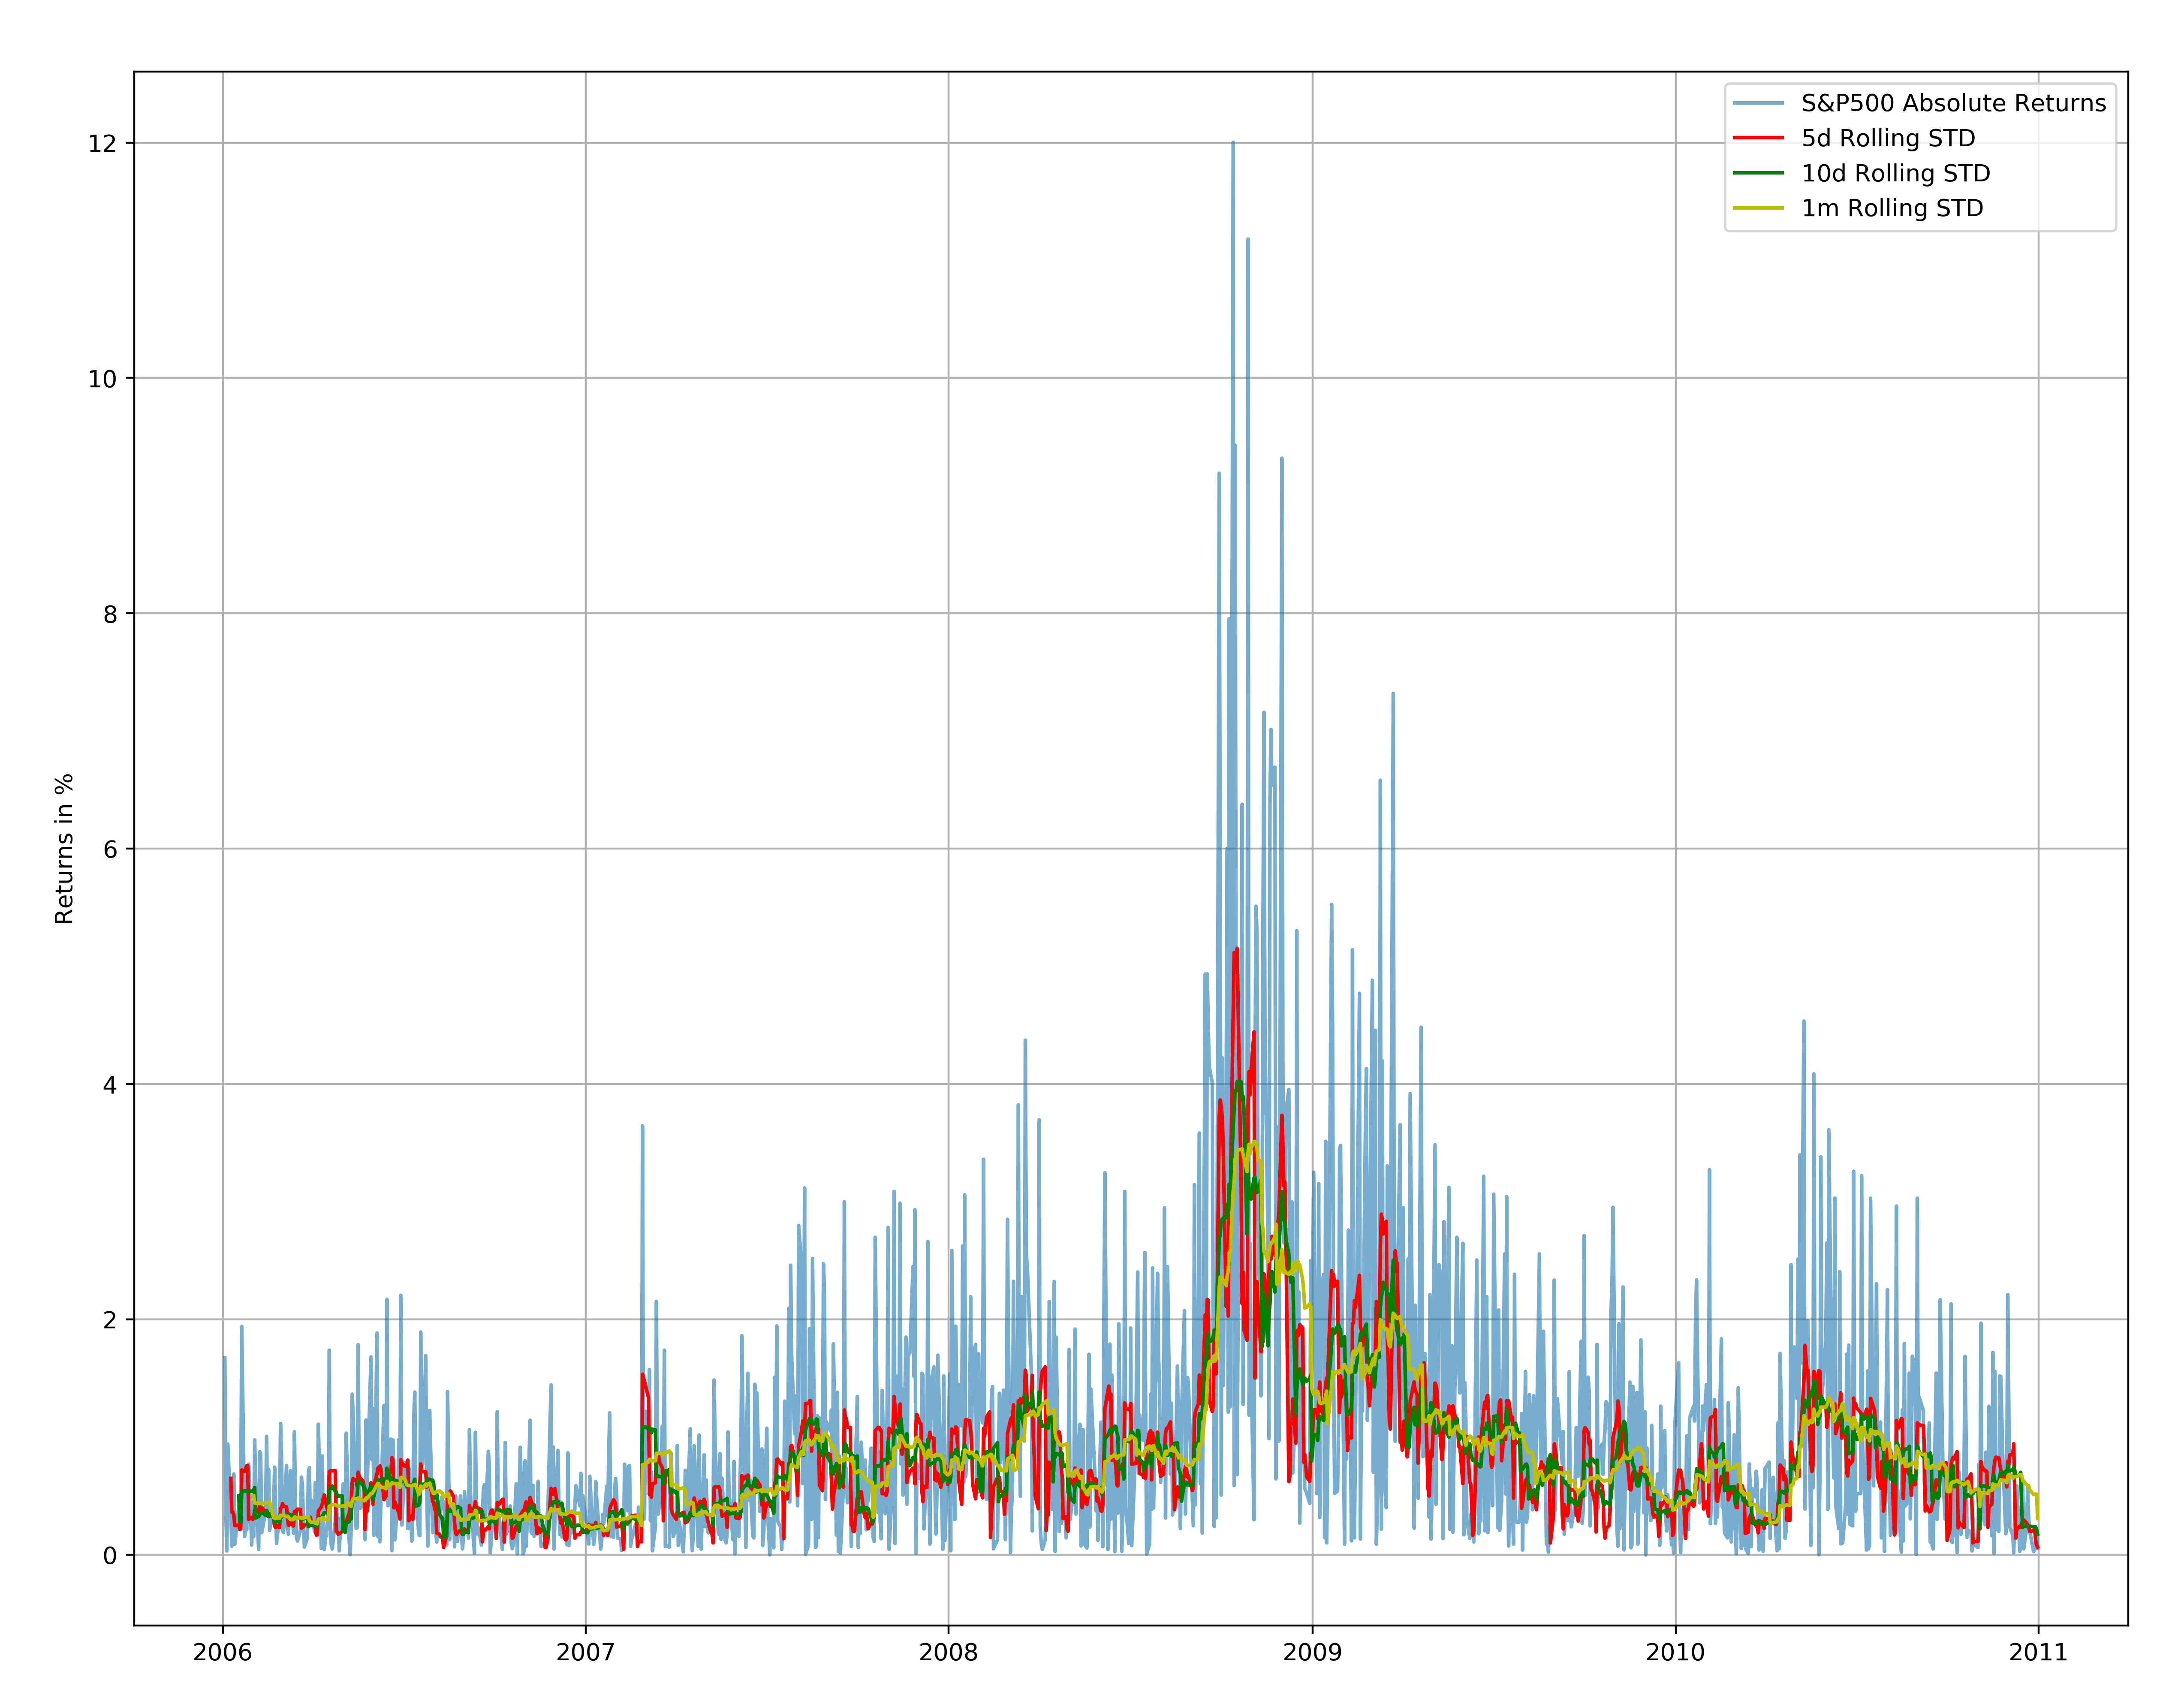
\includegraphics[width=\textwidth]{abs_sp500_returns.png}
\end{figure}
\end{frame}


\begin{frame}
\frametitle{Stylized Facts}
Further analysis of $\{X_t\}$ reveals other kinds of structure that cannot be explained by the gaussian assumption.\\
\vspace{0.5cm}
In particular, the return series displays the following distinctive behavior:

\begin{enumerate}
\item{$\{X_t\}$ is heavy-tailed, much more so than the Gaussian white noise}
\item{Although $\{X_t\}$ is uncorrelated, the series $\{X_{t}^2\}$ is highly correlated}
\item{The changes in $\{X_t\}$ tend to be clustered, large changes tend to be followed by large changes and vice v}
\item{Effects are asymmetric, bad news results in larger downward price moves than positive news does to upward price moves}
\end{enumerate}
\end{frame}

\begin{frame}
\frametitle{S\&P500 Daily Returns (1950-2018)}
\begin{figure}[h!]
\centering 
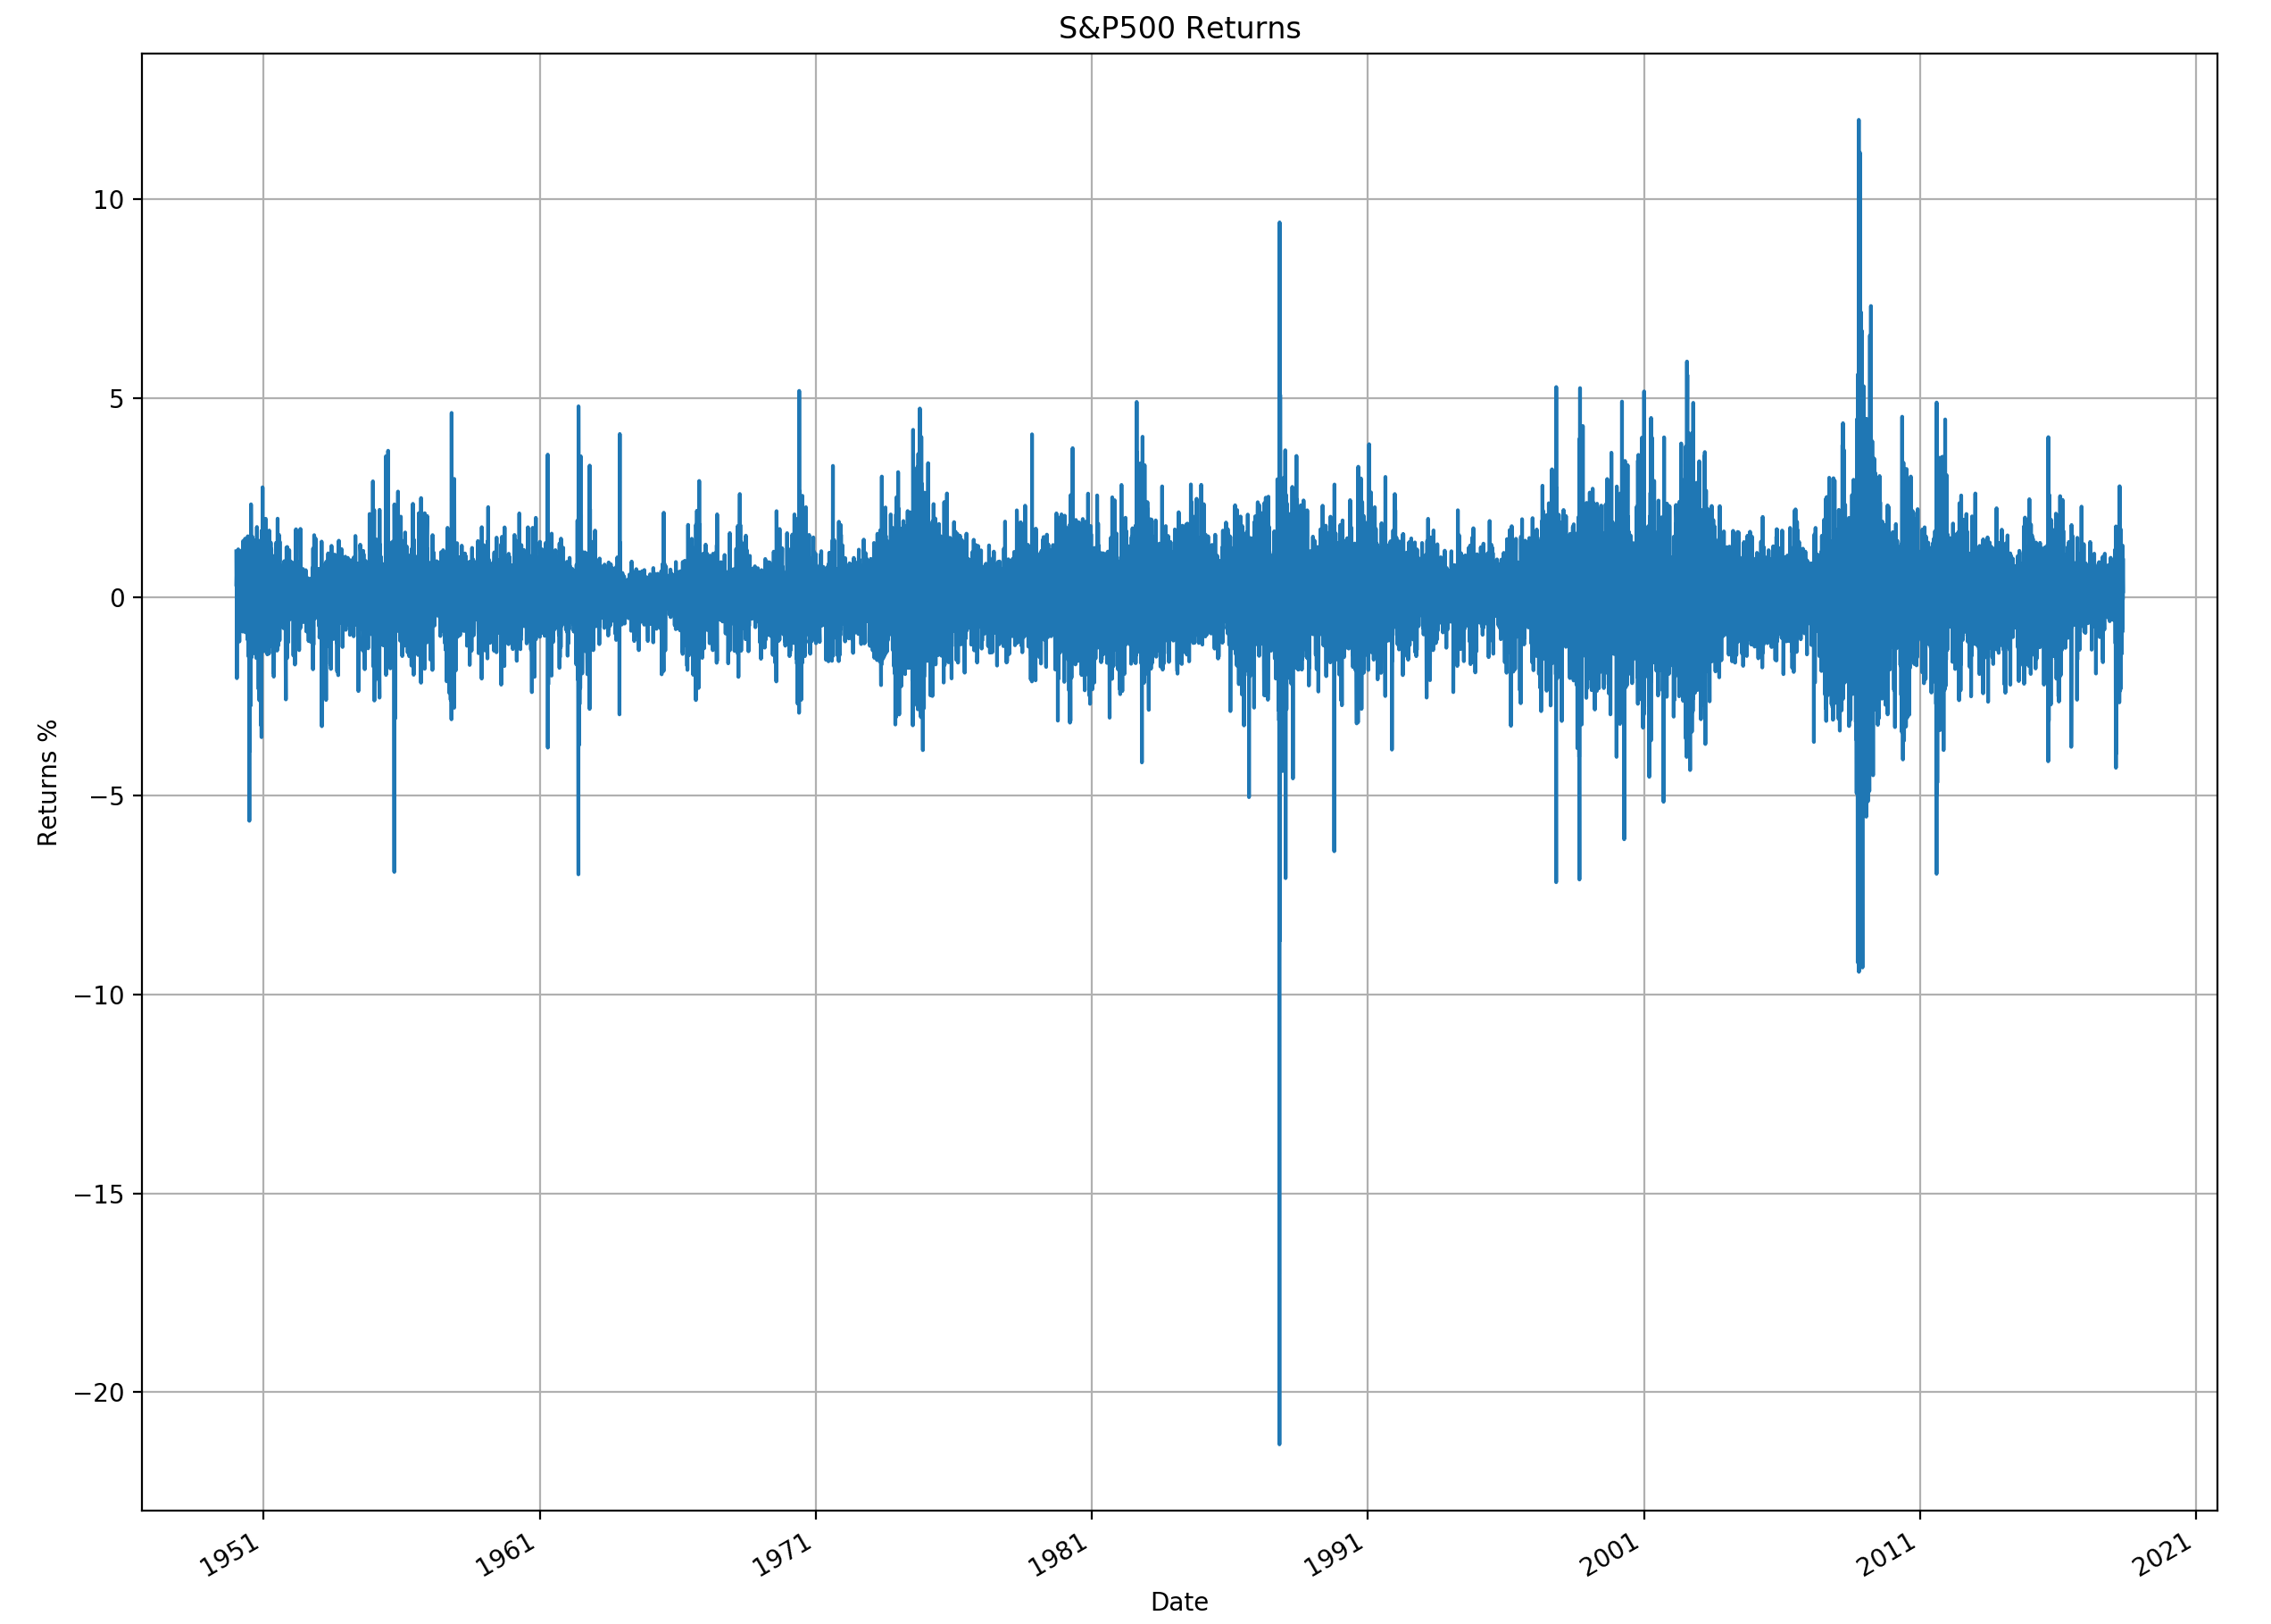
\includegraphics[width=\textwidth]{sp500_returns.png}
\end{figure}
\end{frame}


\begin{frame}
\frametitle{GARCH}
The Generalized ARCH (GARCH) model of Bollerslev (1986) and it's variants are extremely popular (albeit imperfect) methods to model volatility.\\
\vspace{15pt}
GARCH(p,q) model can be expressed as:

$$ X_t = \sigma_{t}\epsilon_{t}, \hspace{15pt} \epsilon_{t} \sim N(0,1) $$
where $$\sigma_{t}^{2} = \a_0 + \sum_{i=1}^{p} \beta_i \sigma_{t-i}^{2} + \sum_{j=1}^{q} \a_j X_{t-j}^{2}$$

For the purposes of this talk, we'll focus on GARCH(1,1) models where $\sigma_{t}^{2} = \a_0 + \beta_1 \sigma_{t-1}^{2} + \a_1 X_{t-1}^{2}$
\end{frame}

\section{Normalizing and Variance Stabilizing (NoVaS) Transformation}

\begin{frame}
\frametitle{Outline}
\tableofcontents[currentsection]
\end{frame}

\begin{frame}
\frametitle{NoVaS Transformation (Politis 2007)}
The NoVaS Transformation is defined as $$ W_{t,a} = \frac{X_t}{\sqrt{\alpha s^2_{t-1} + a_0 X^2_{t} + \sum_{i=1}^{p} a_i X^2_{t-i}}}$$ for $t=p+1,p+2,\dots,n$ \\
\vspace{3pt}
It is a clever extension of the ARCH model where we include the value $X_t$ in order to ``studentize'' the returns.\\
\vspace{5pt}
The order $p$ and the vector of nonnegative parameters $(\a,a_0,\dots,a_p)$ are chosen by the practitioner with the twin goals of normalization and variance-stabilization.\\
\vspace{5pt}
Algorithm for Simple NoVaS:
\begin{itemize}
\item{Let $\a = 0$ and $a_i = \frac{1}{p+1}$ for all $0 \leq i \leq p$}
\item{Pick $p$ such that $|KURT_{n}(W_{t,p}^{S})| \approx 3$}
\end{itemize}




\end{frame}


%% S&P 500 %%
\begin{frame}
\frametitle{S\&P500 Daily Returns (1950-2018)}
\begin{figure}[h!]
\centering 
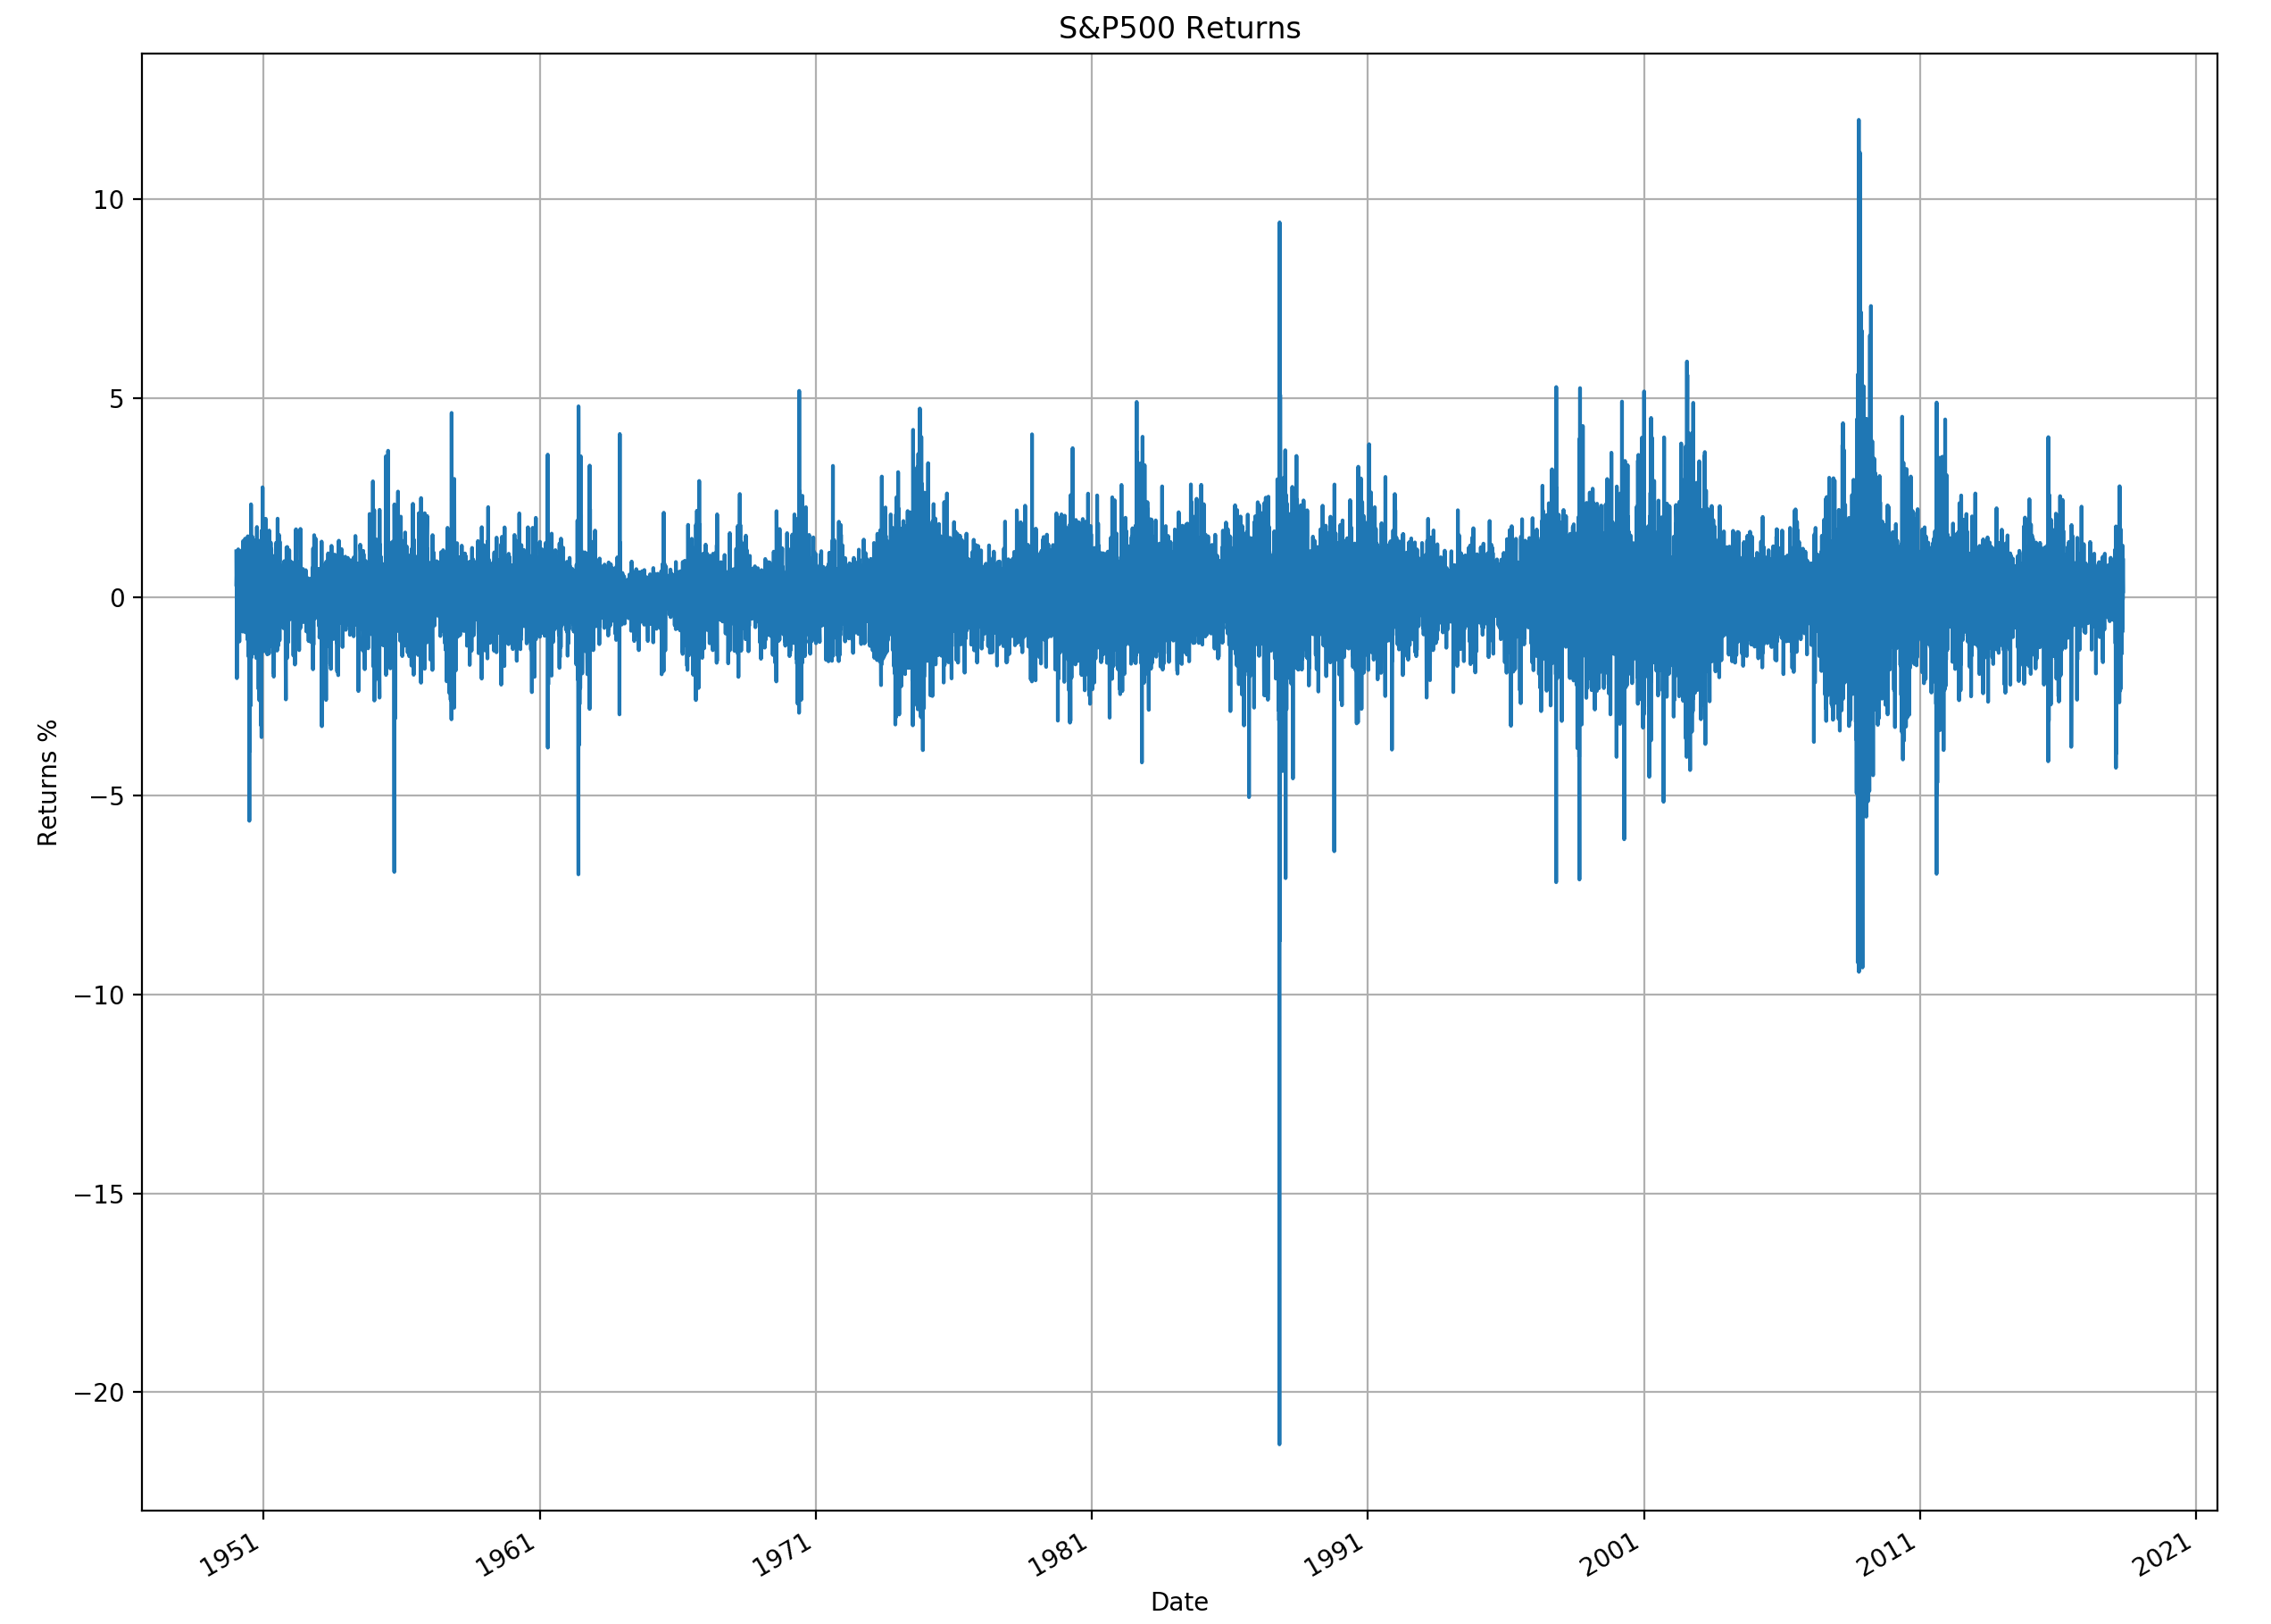
\includegraphics[width=\textwidth]{sp500_returns.png}
\end{figure}
\end{frame}

\begin{frame}
\frametitle{S\&P500 Daily Returns Histogram}
\begin{figure}[h!]
\centering 
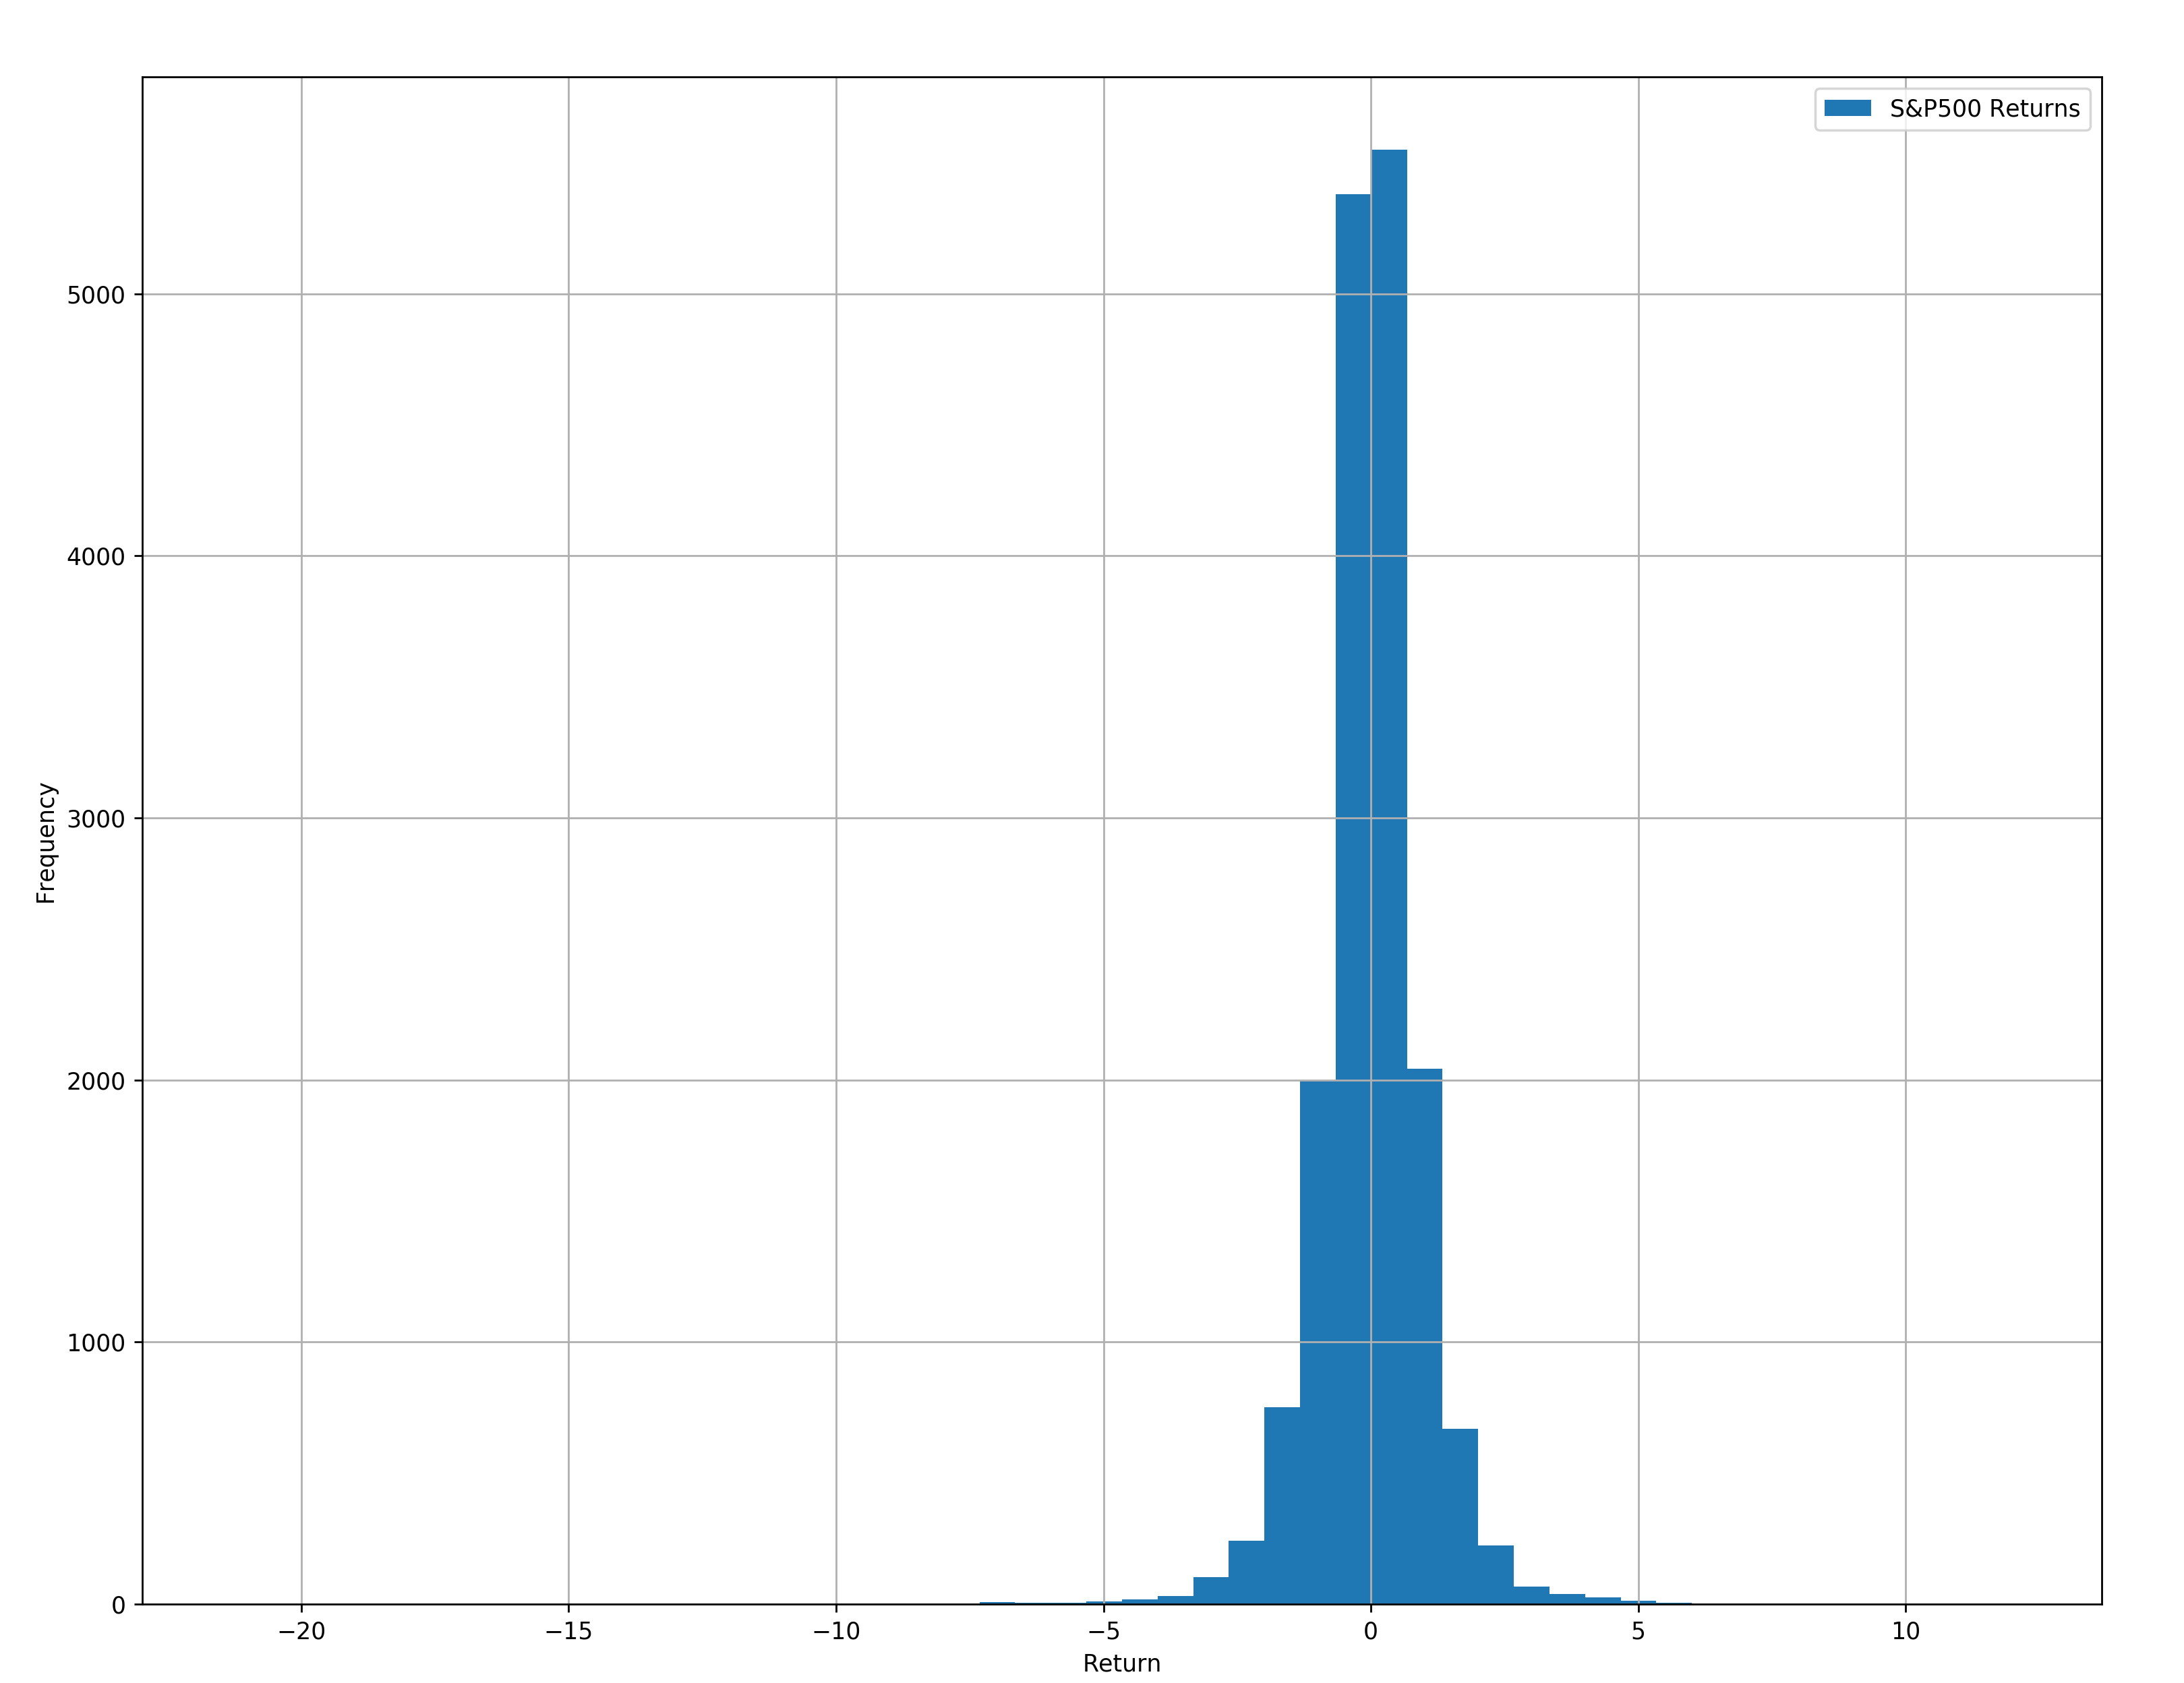
\includegraphics[width=\textwidth]{sp500_returns_hist.png}
\end{figure}
\end{frame}

\begin{frame}
\frametitle{S\&P500 Daily Returns Q-Q Plot}
\begin{figure}[h!]
\centering 
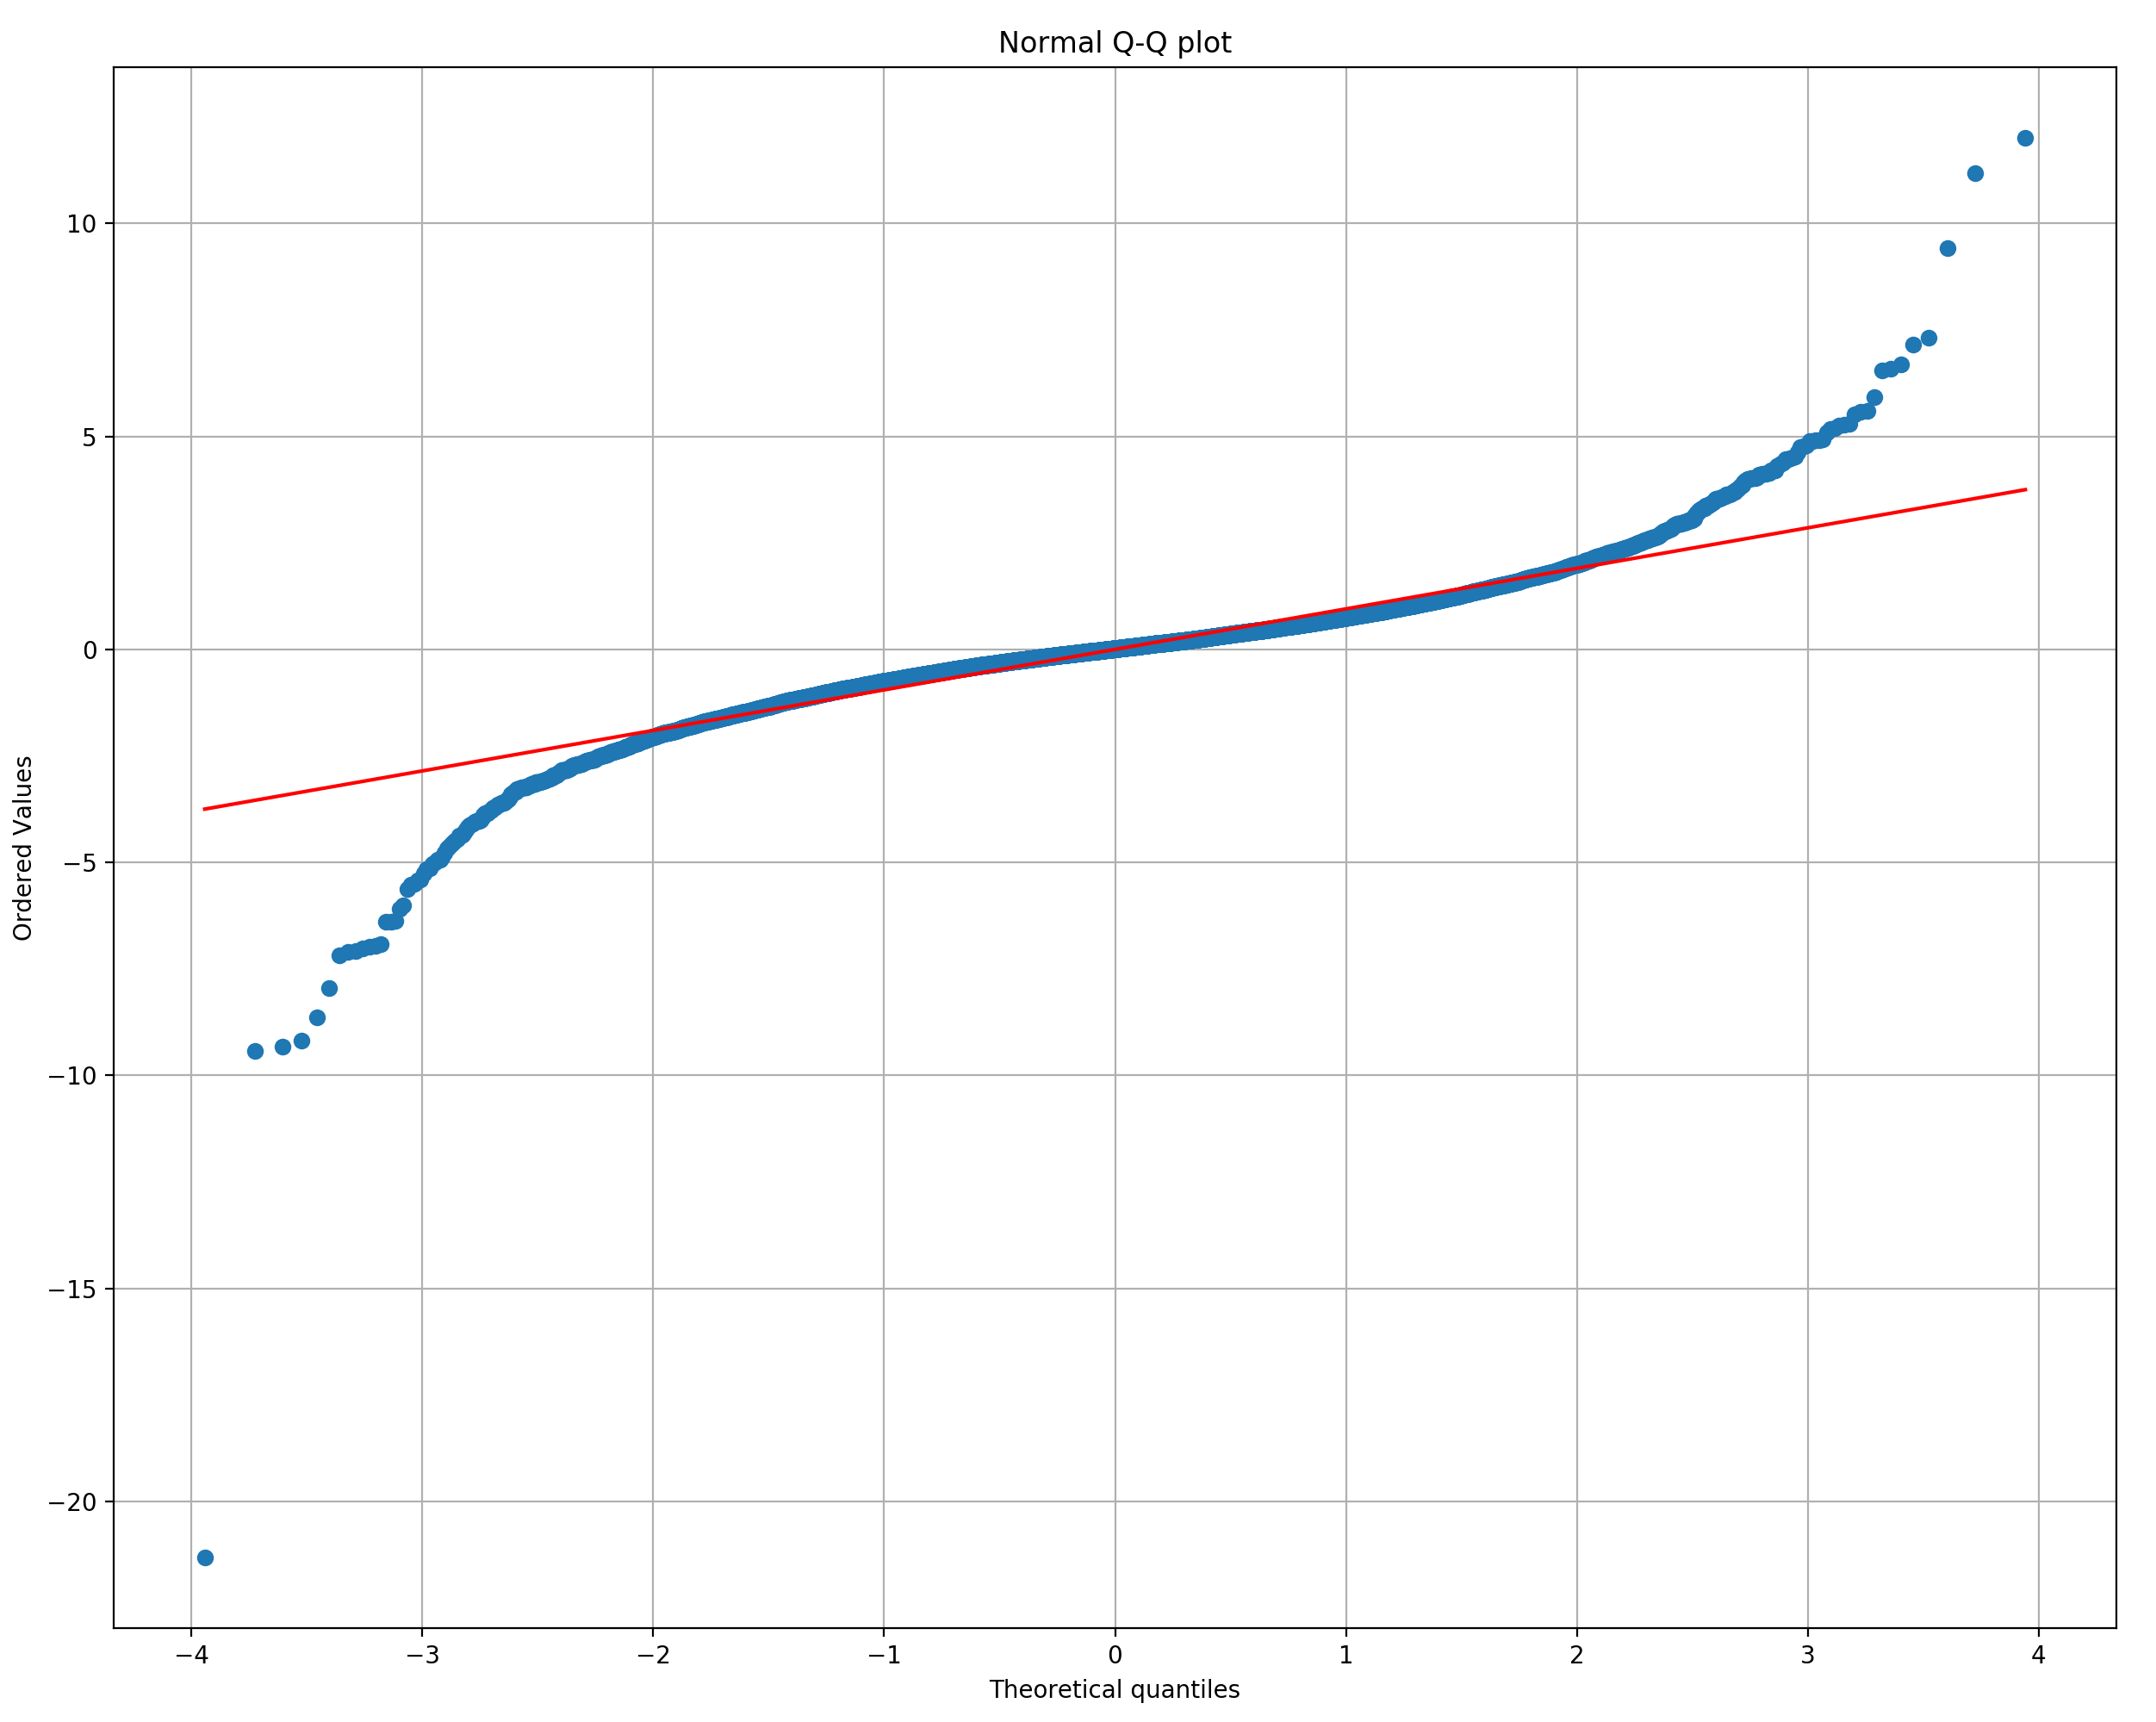
\includegraphics[width=\textwidth]{sp500_returns_qqplot.png}
\end{figure}
\end{frame}

\begin{frame}
\frametitle{NoVaS Transformed S\&P500 Daily Returns (p=16)}
\begin{figure}[h!]
\centering 
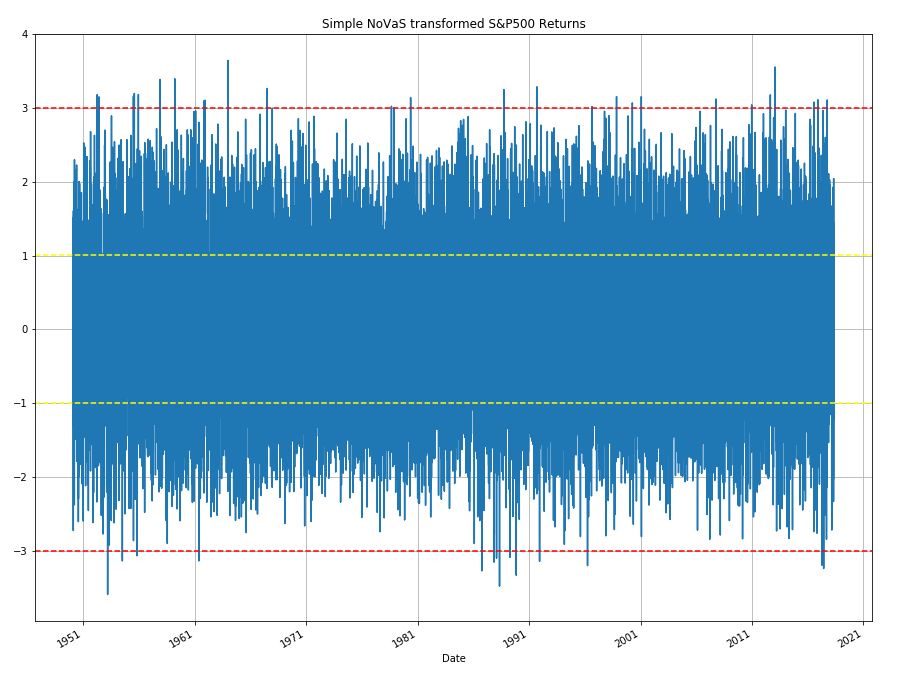
\includegraphics[width=\textwidth]{novas_sp500_returns.png}
\end{figure}
\end{frame}

\begin{frame}
\frametitle{NoVaS Transformed S\&P500 Histogram (p=16)}
\begin{figure}[h!]
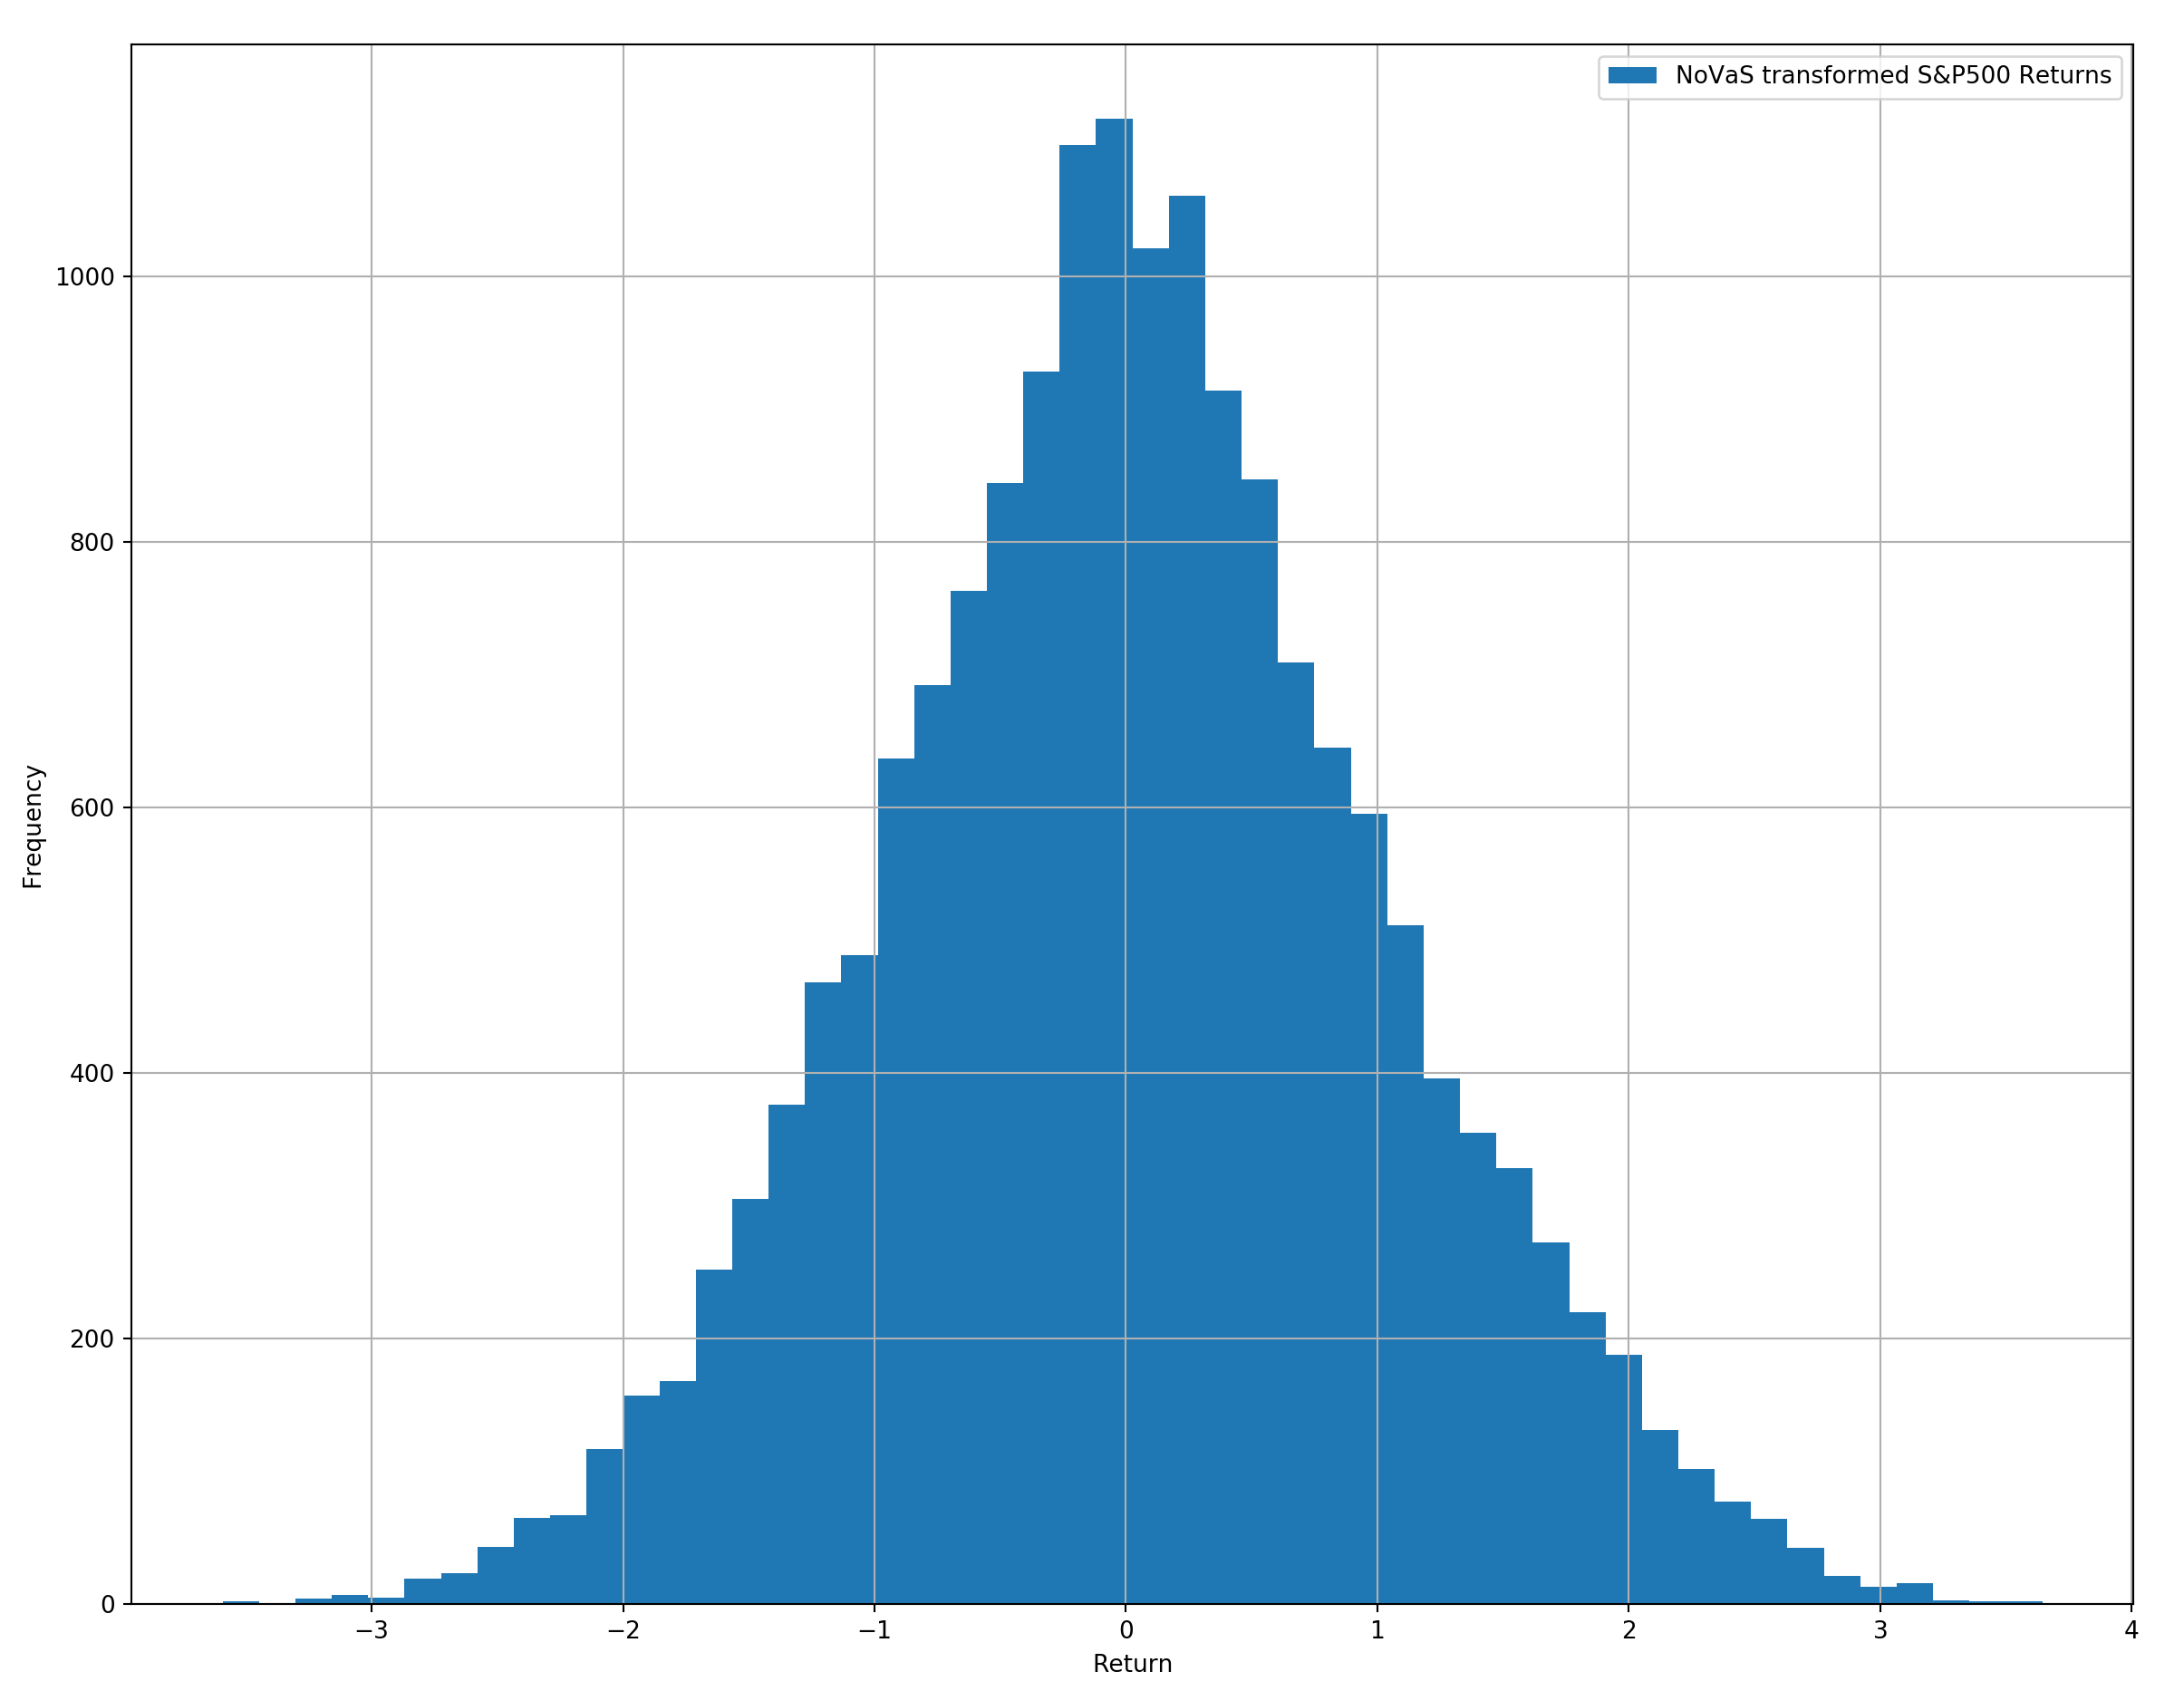
\includegraphics[width=\textwidth]{novas_sp500_returns_hist.png}
\end{figure}
\end{frame}

\begin{frame}
\frametitle{NoVaS Transformed S\&P500 QQ-Plot (p=16)}
\begin{figure}[h!]
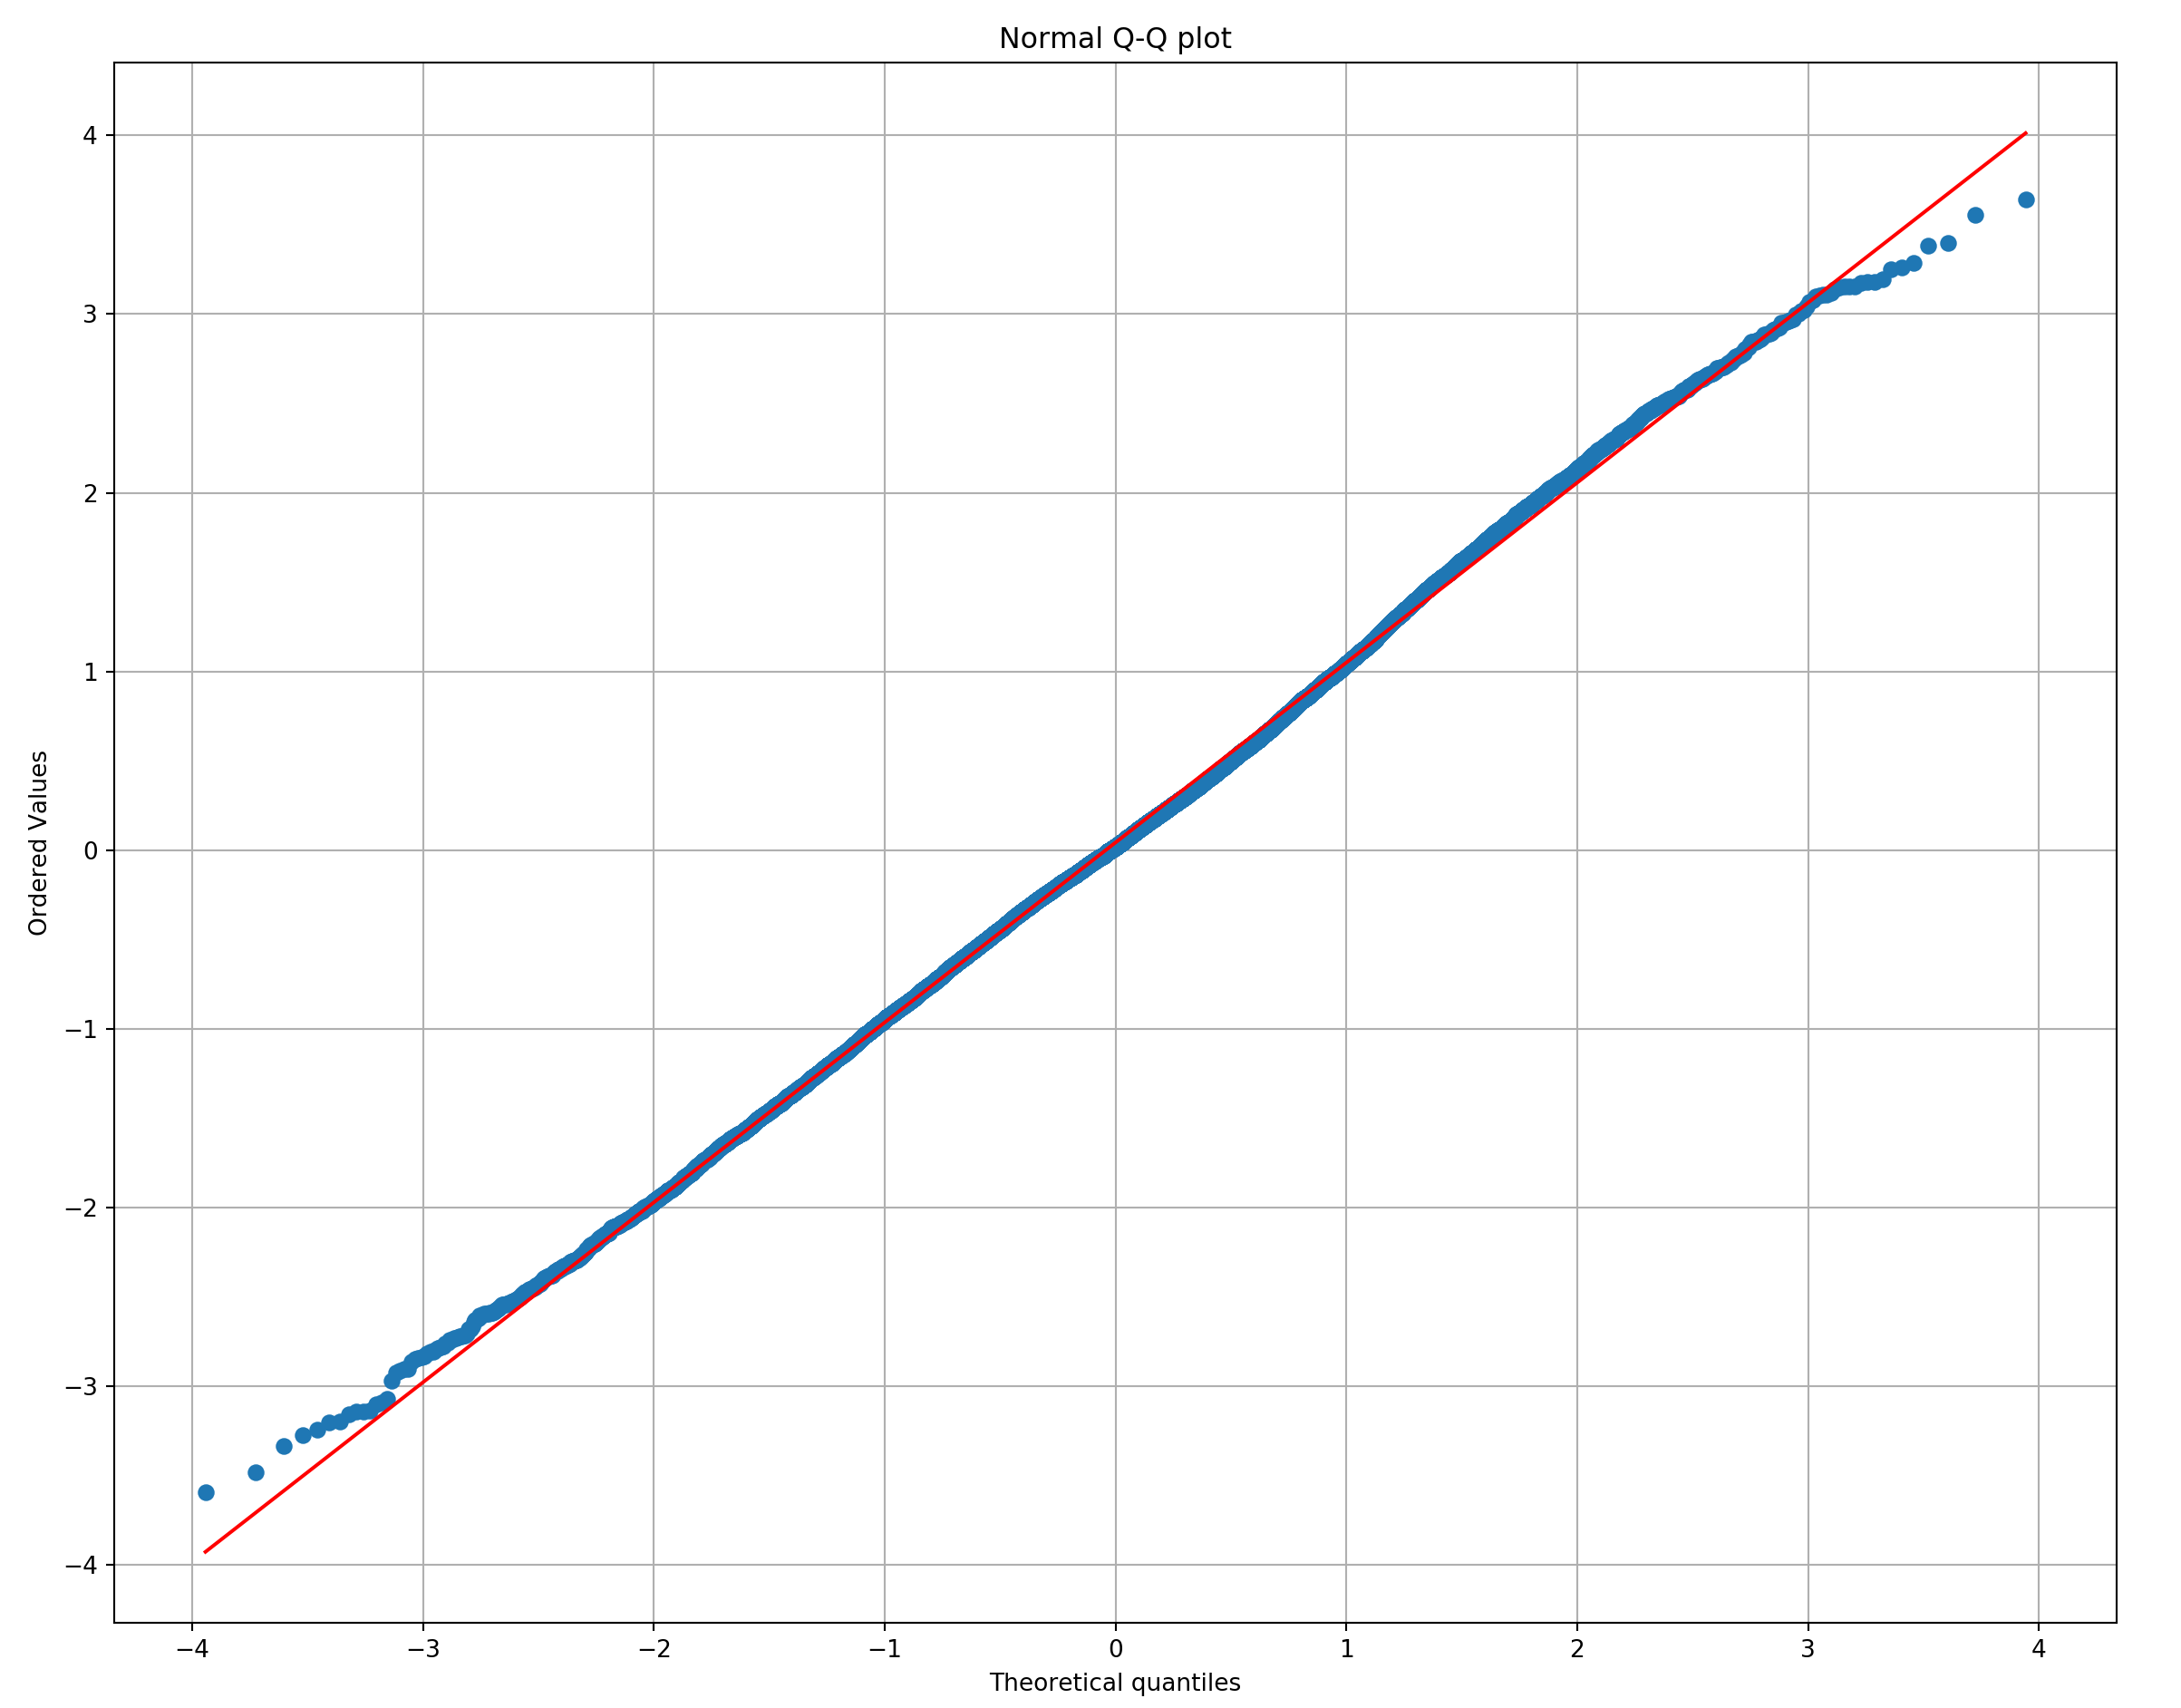
\includegraphics[width=\textwidth]{novas_sp500_returns_qqplot.png}
\end{figure}
\end{frame}

%%%%%%%%%%%%%%%%%%%
%%%%%%% BTC %%%%%%%
%%%%%%%%%%%%%%%%%%%

\begin{frame}
\frametitle{BTC/USD Daily Returns (2010-2018)}
\begin{figure}[h!]
\centering 
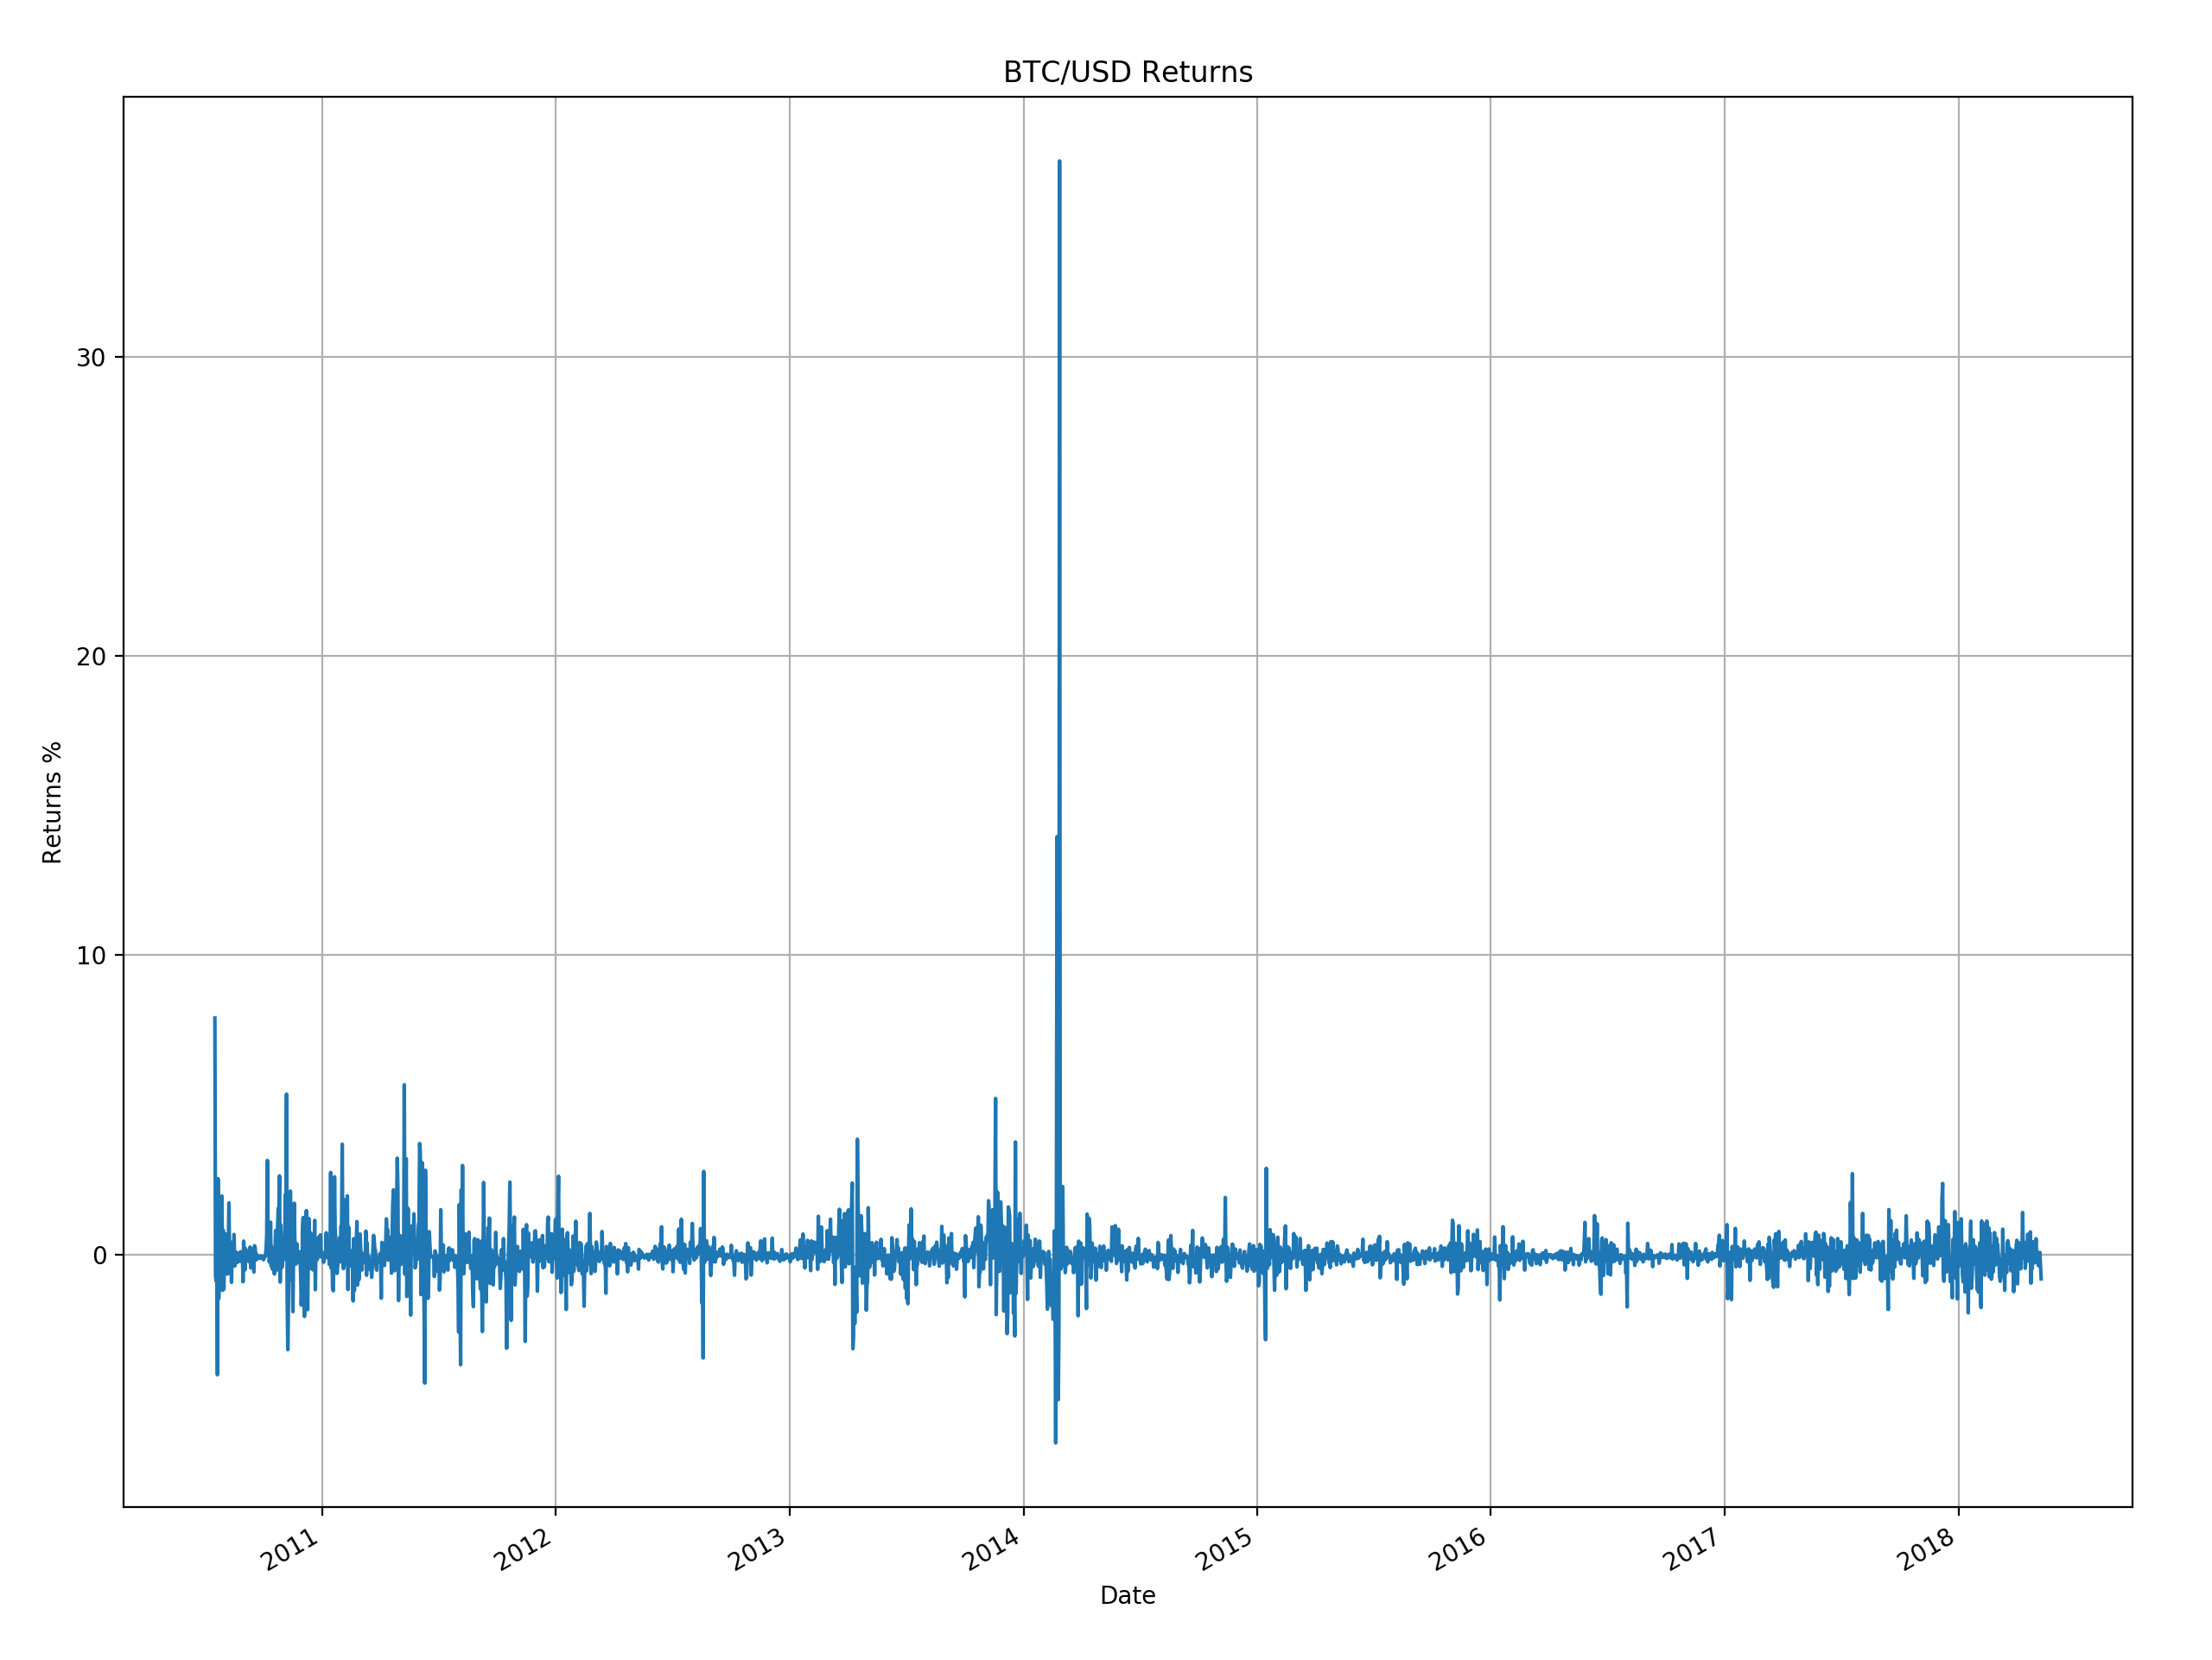
\includegraphics[width=\textwidth]{btc_returns.png}
\end{figure}
\end{frame}

\begin{frame}
\frametitle{BTC/USD Daily Returns Histogram (2010-2018)}
\begin{figure}[h!]
\centering 
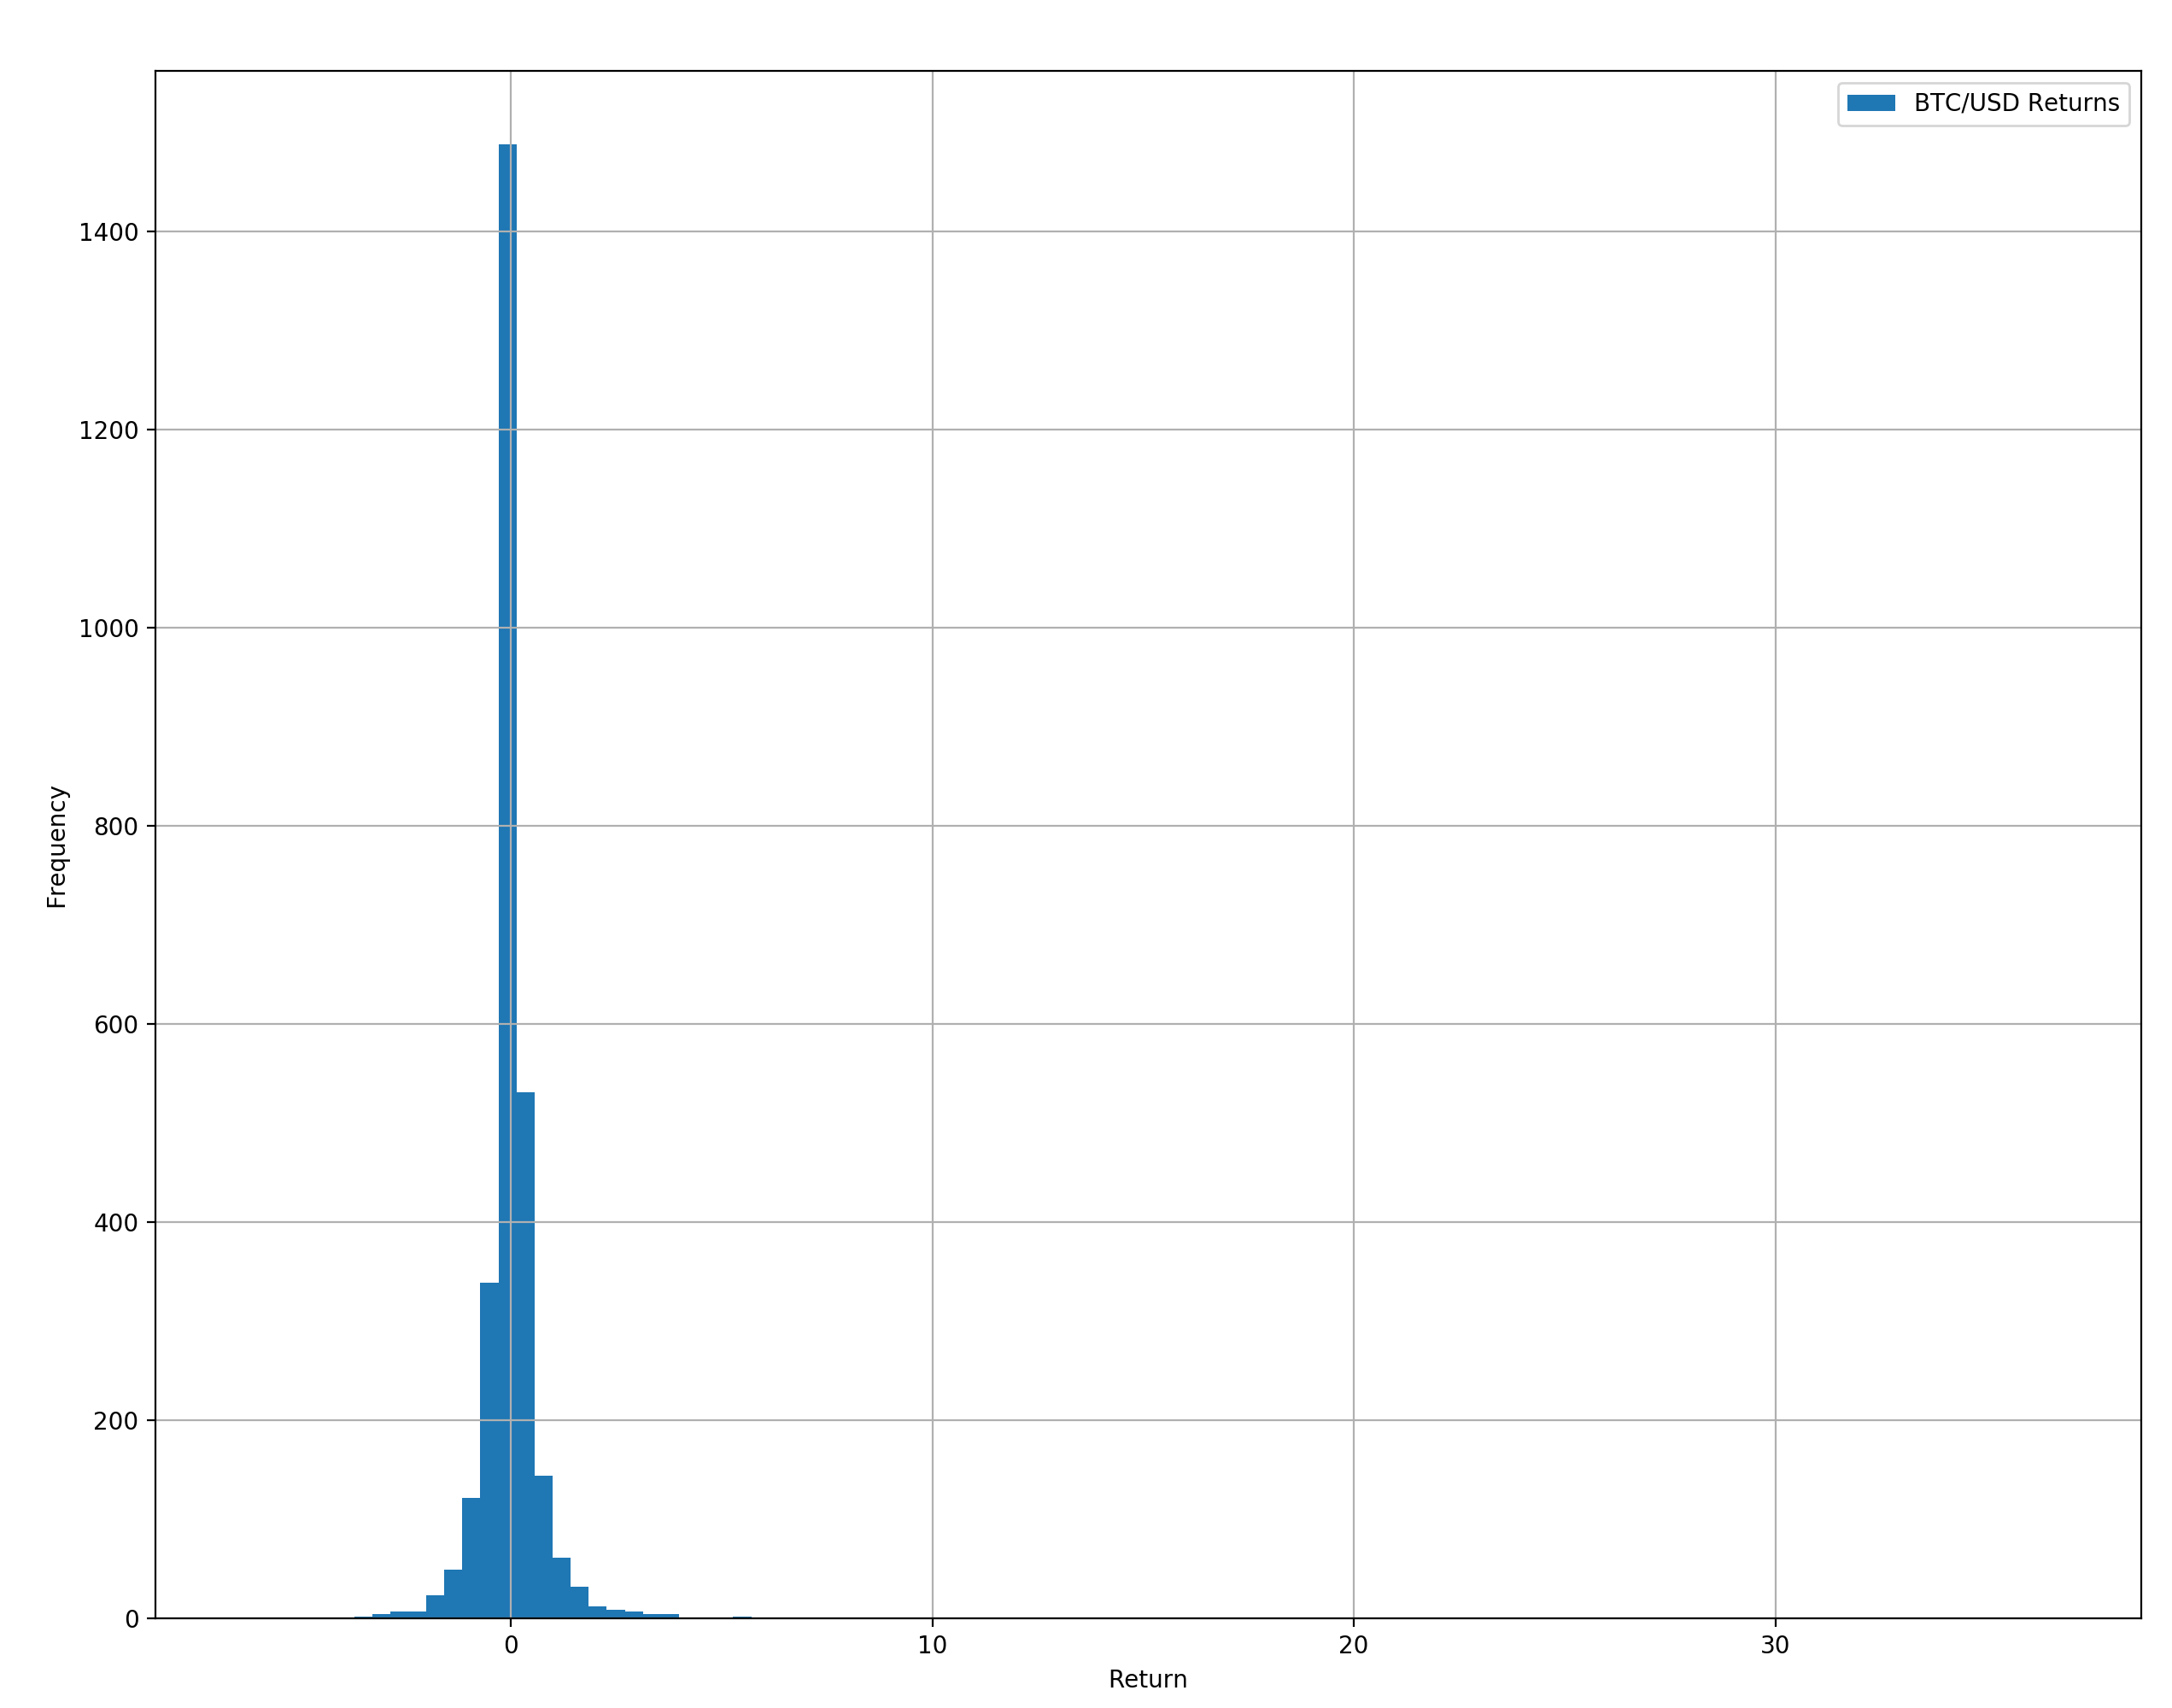
\includegraphics[width=\textwidth]{btc_returns_hist.png}
\end{figure}
\end{frame}

\begin{frame}
\frametitle{BTC/USD Daily Returns QQ-Plot (2010-2018)}
\begin{figure}[h!]
\centering 
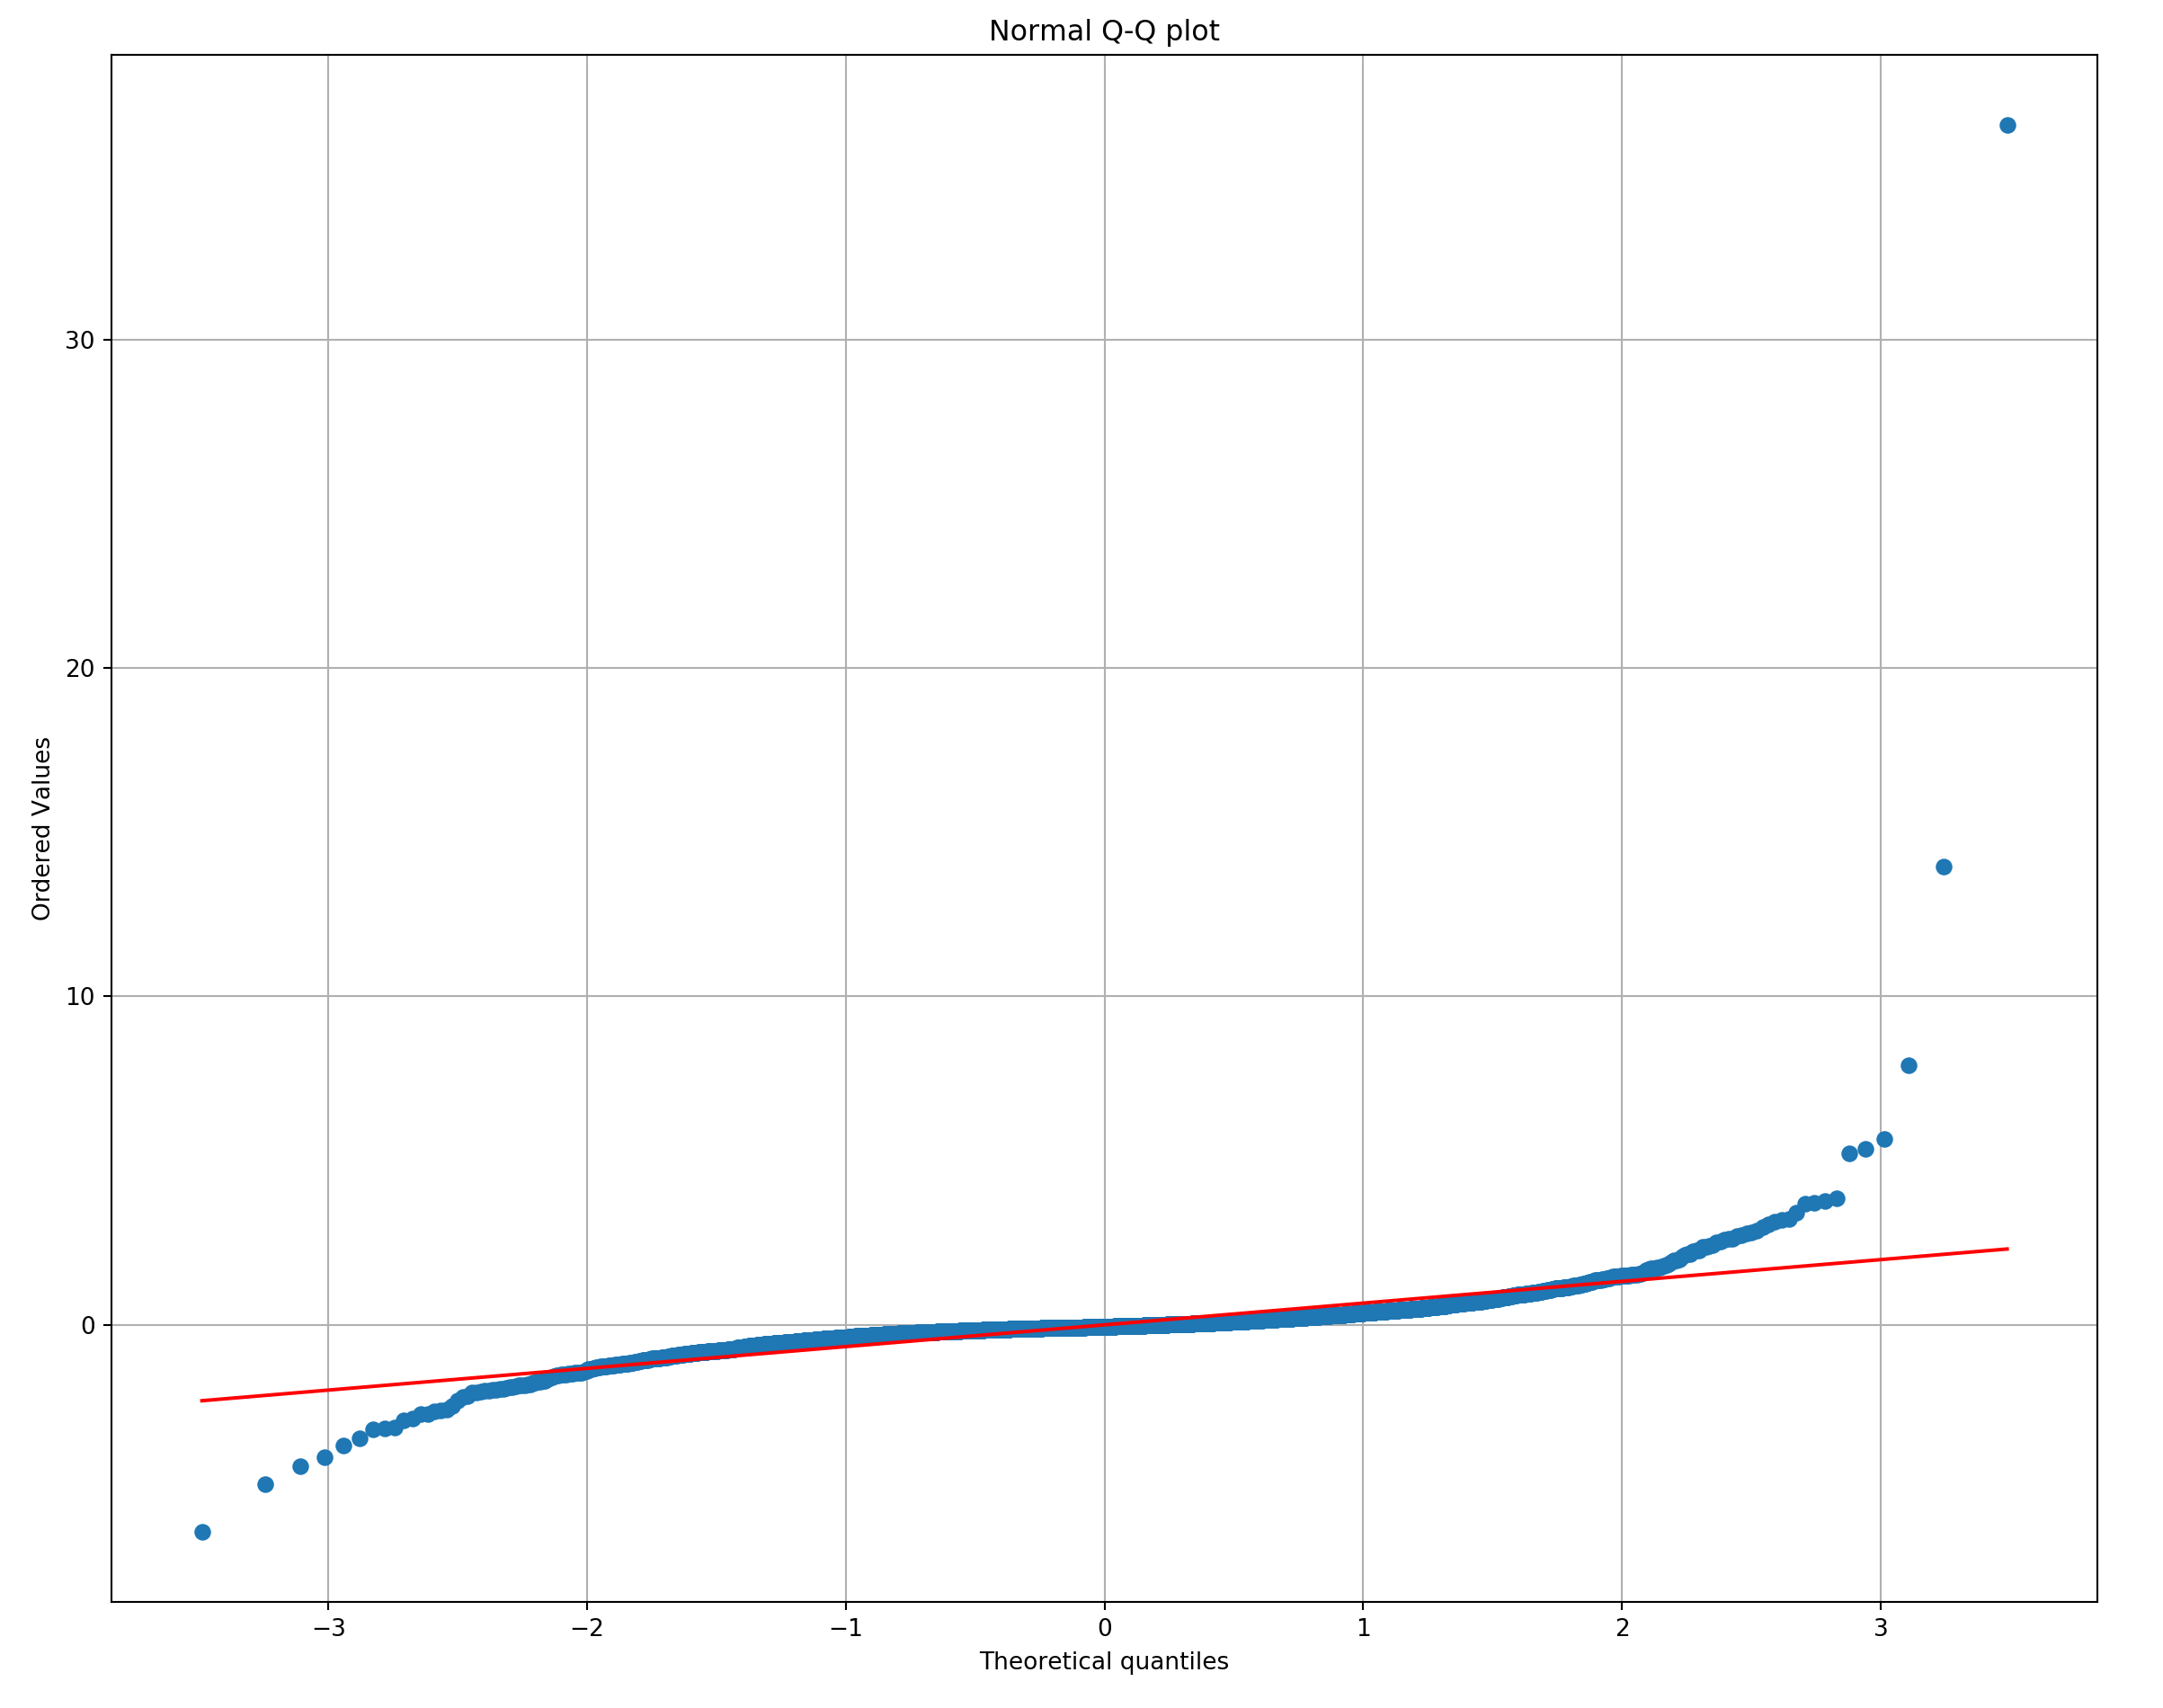
\includegraphics[width=\textwidth]{btc_returns_qqplot.png}
\end{figure}
\end{frame}

\begin{frame}
\frametitle{NoVaS Transformed BTC/USD Returns (p=12)}
\begin{figure}[h!]
\centering 
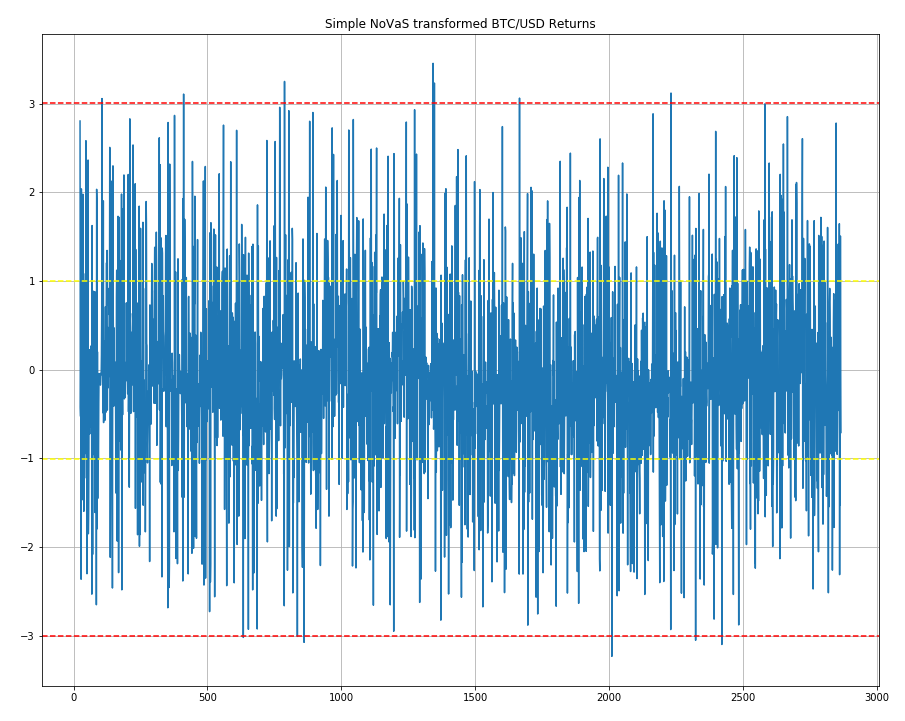
\includegraphics[width=\textwidth]{novas_btc_returns.png}
\end{figure}
\end{frame}

\begin{frame}
\frametitle{NoVaS Transformed BTC/USD Histogram (p=12)}
\begin{figure}[h!]
\centering 
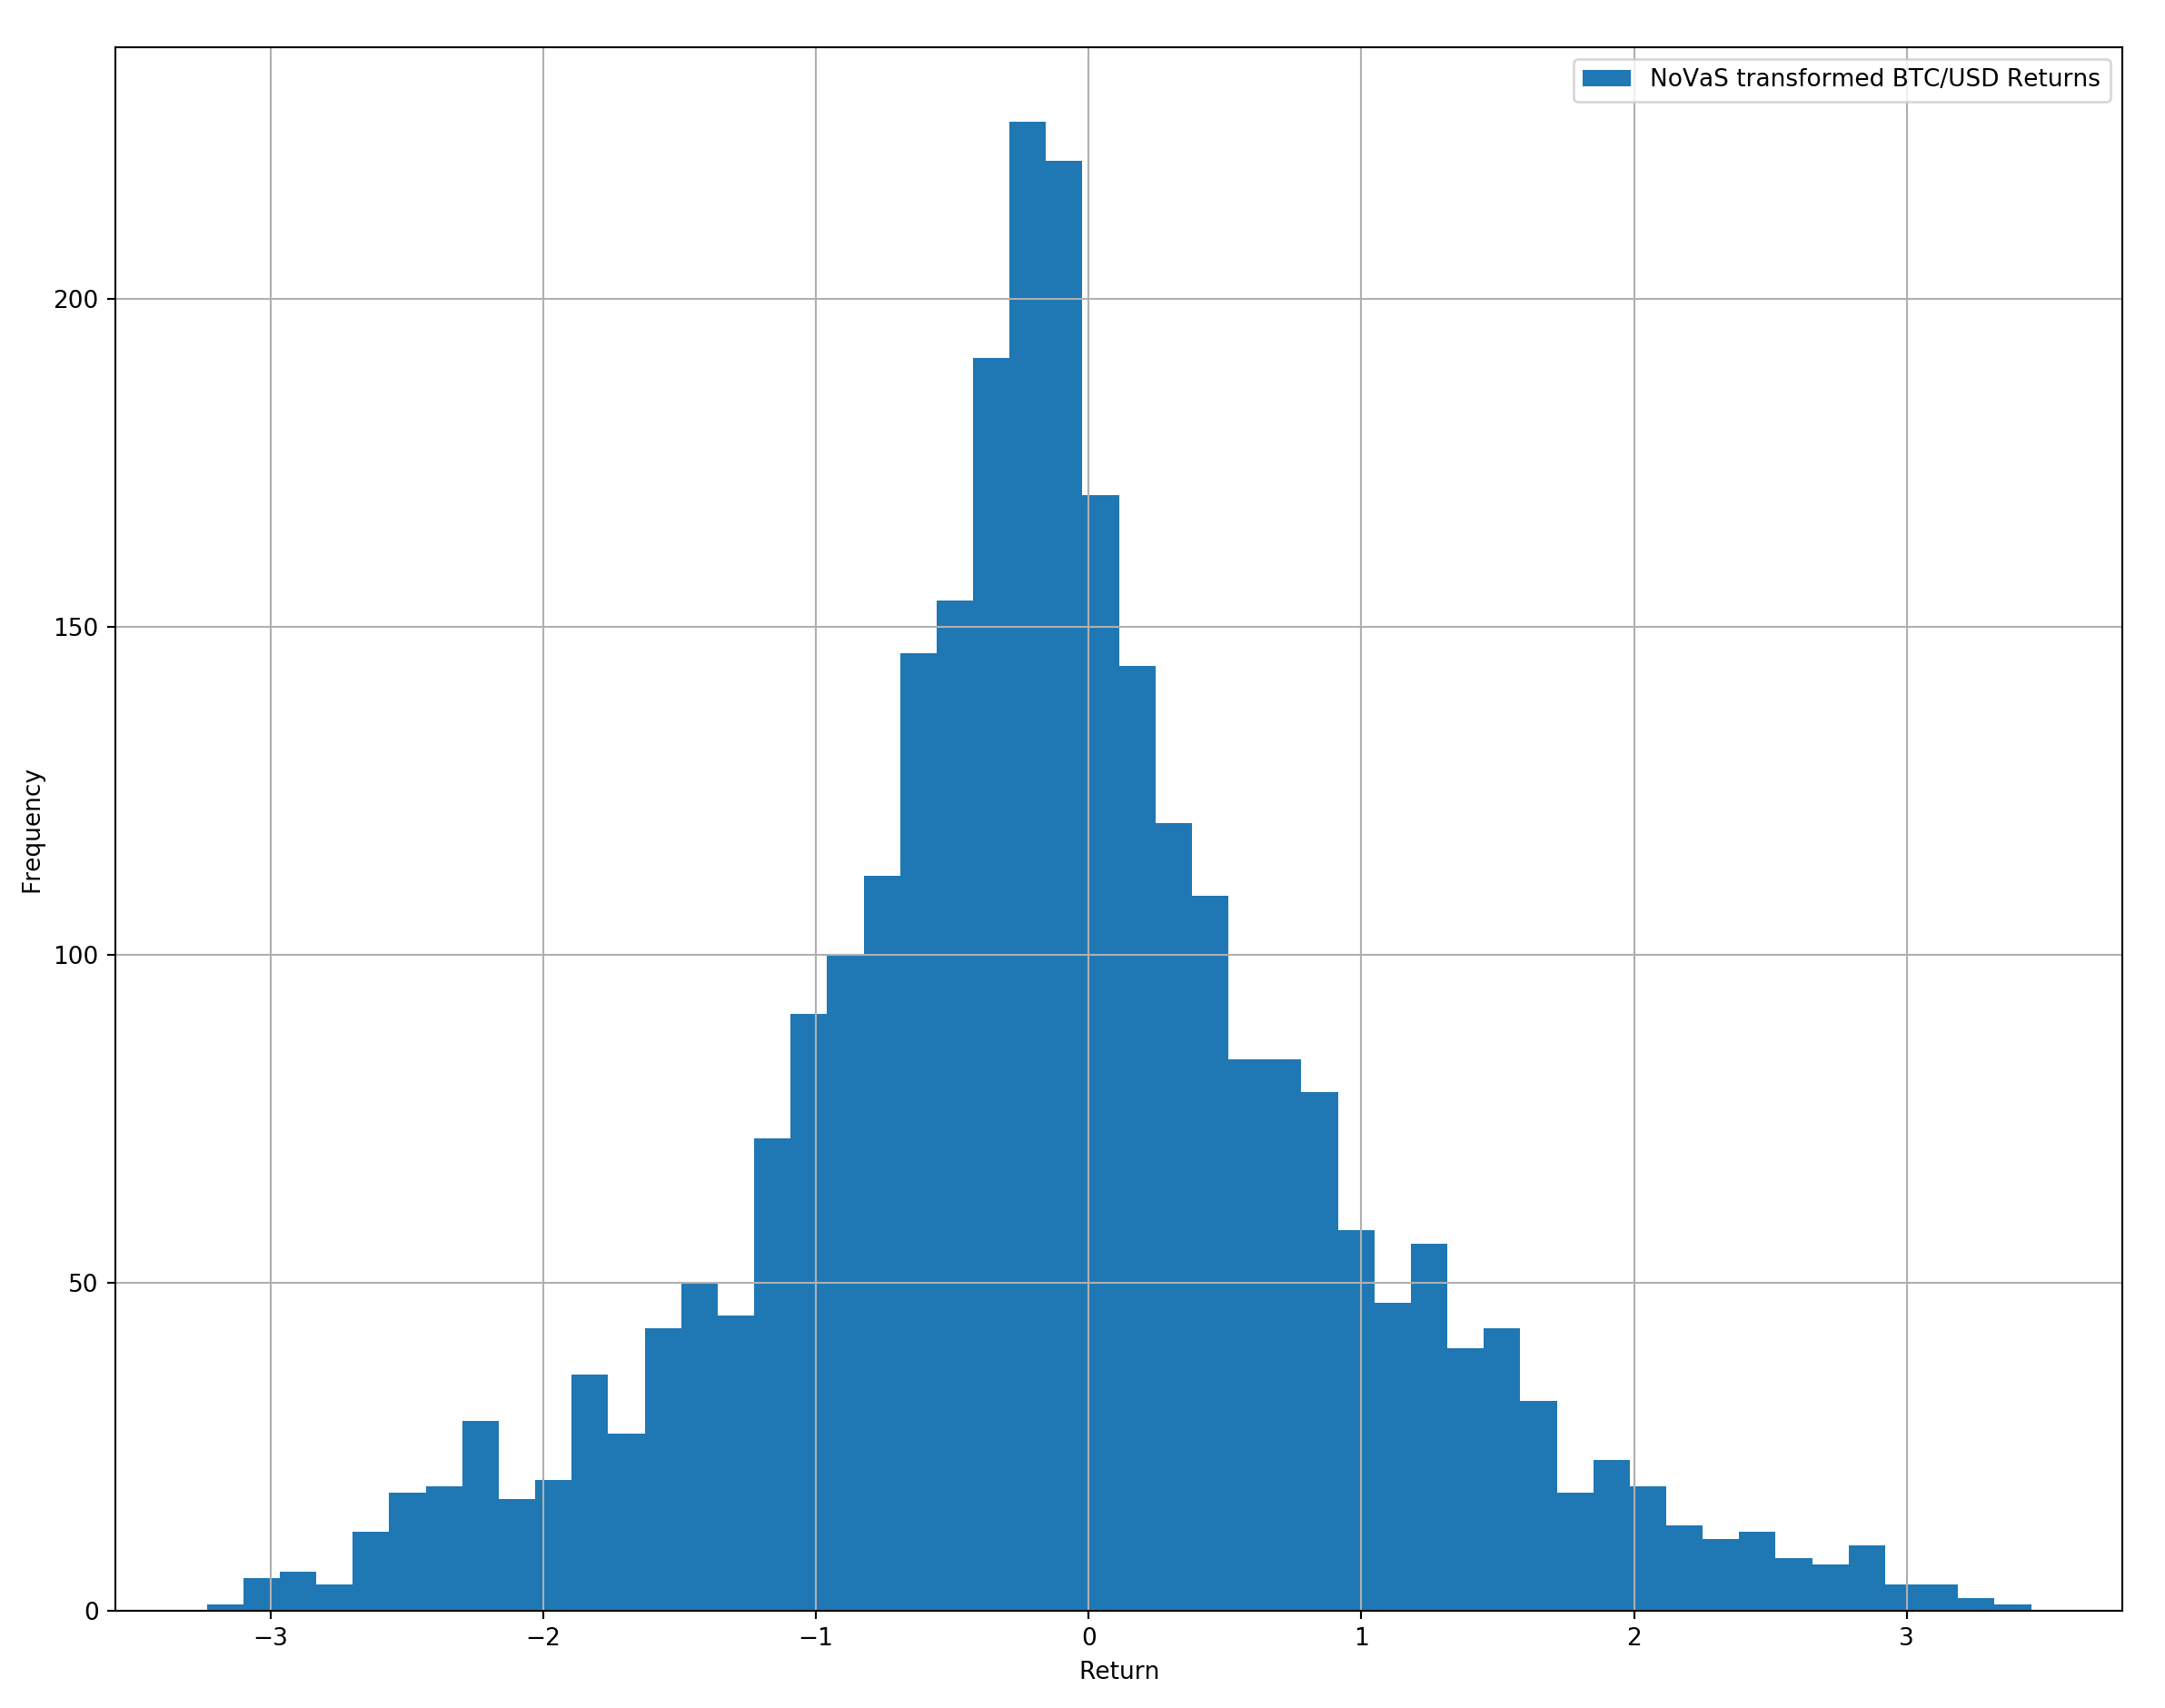
\includegraphics[width=\textwidth]{novas_btc_returns_hist.png}
\end{figure}
\end{frame}

\begin{frame}
\frametitle{NoVaS Transformed BTC/USD QQ-Plot (p=12)}
\begin{figure}[h!]
\centering 
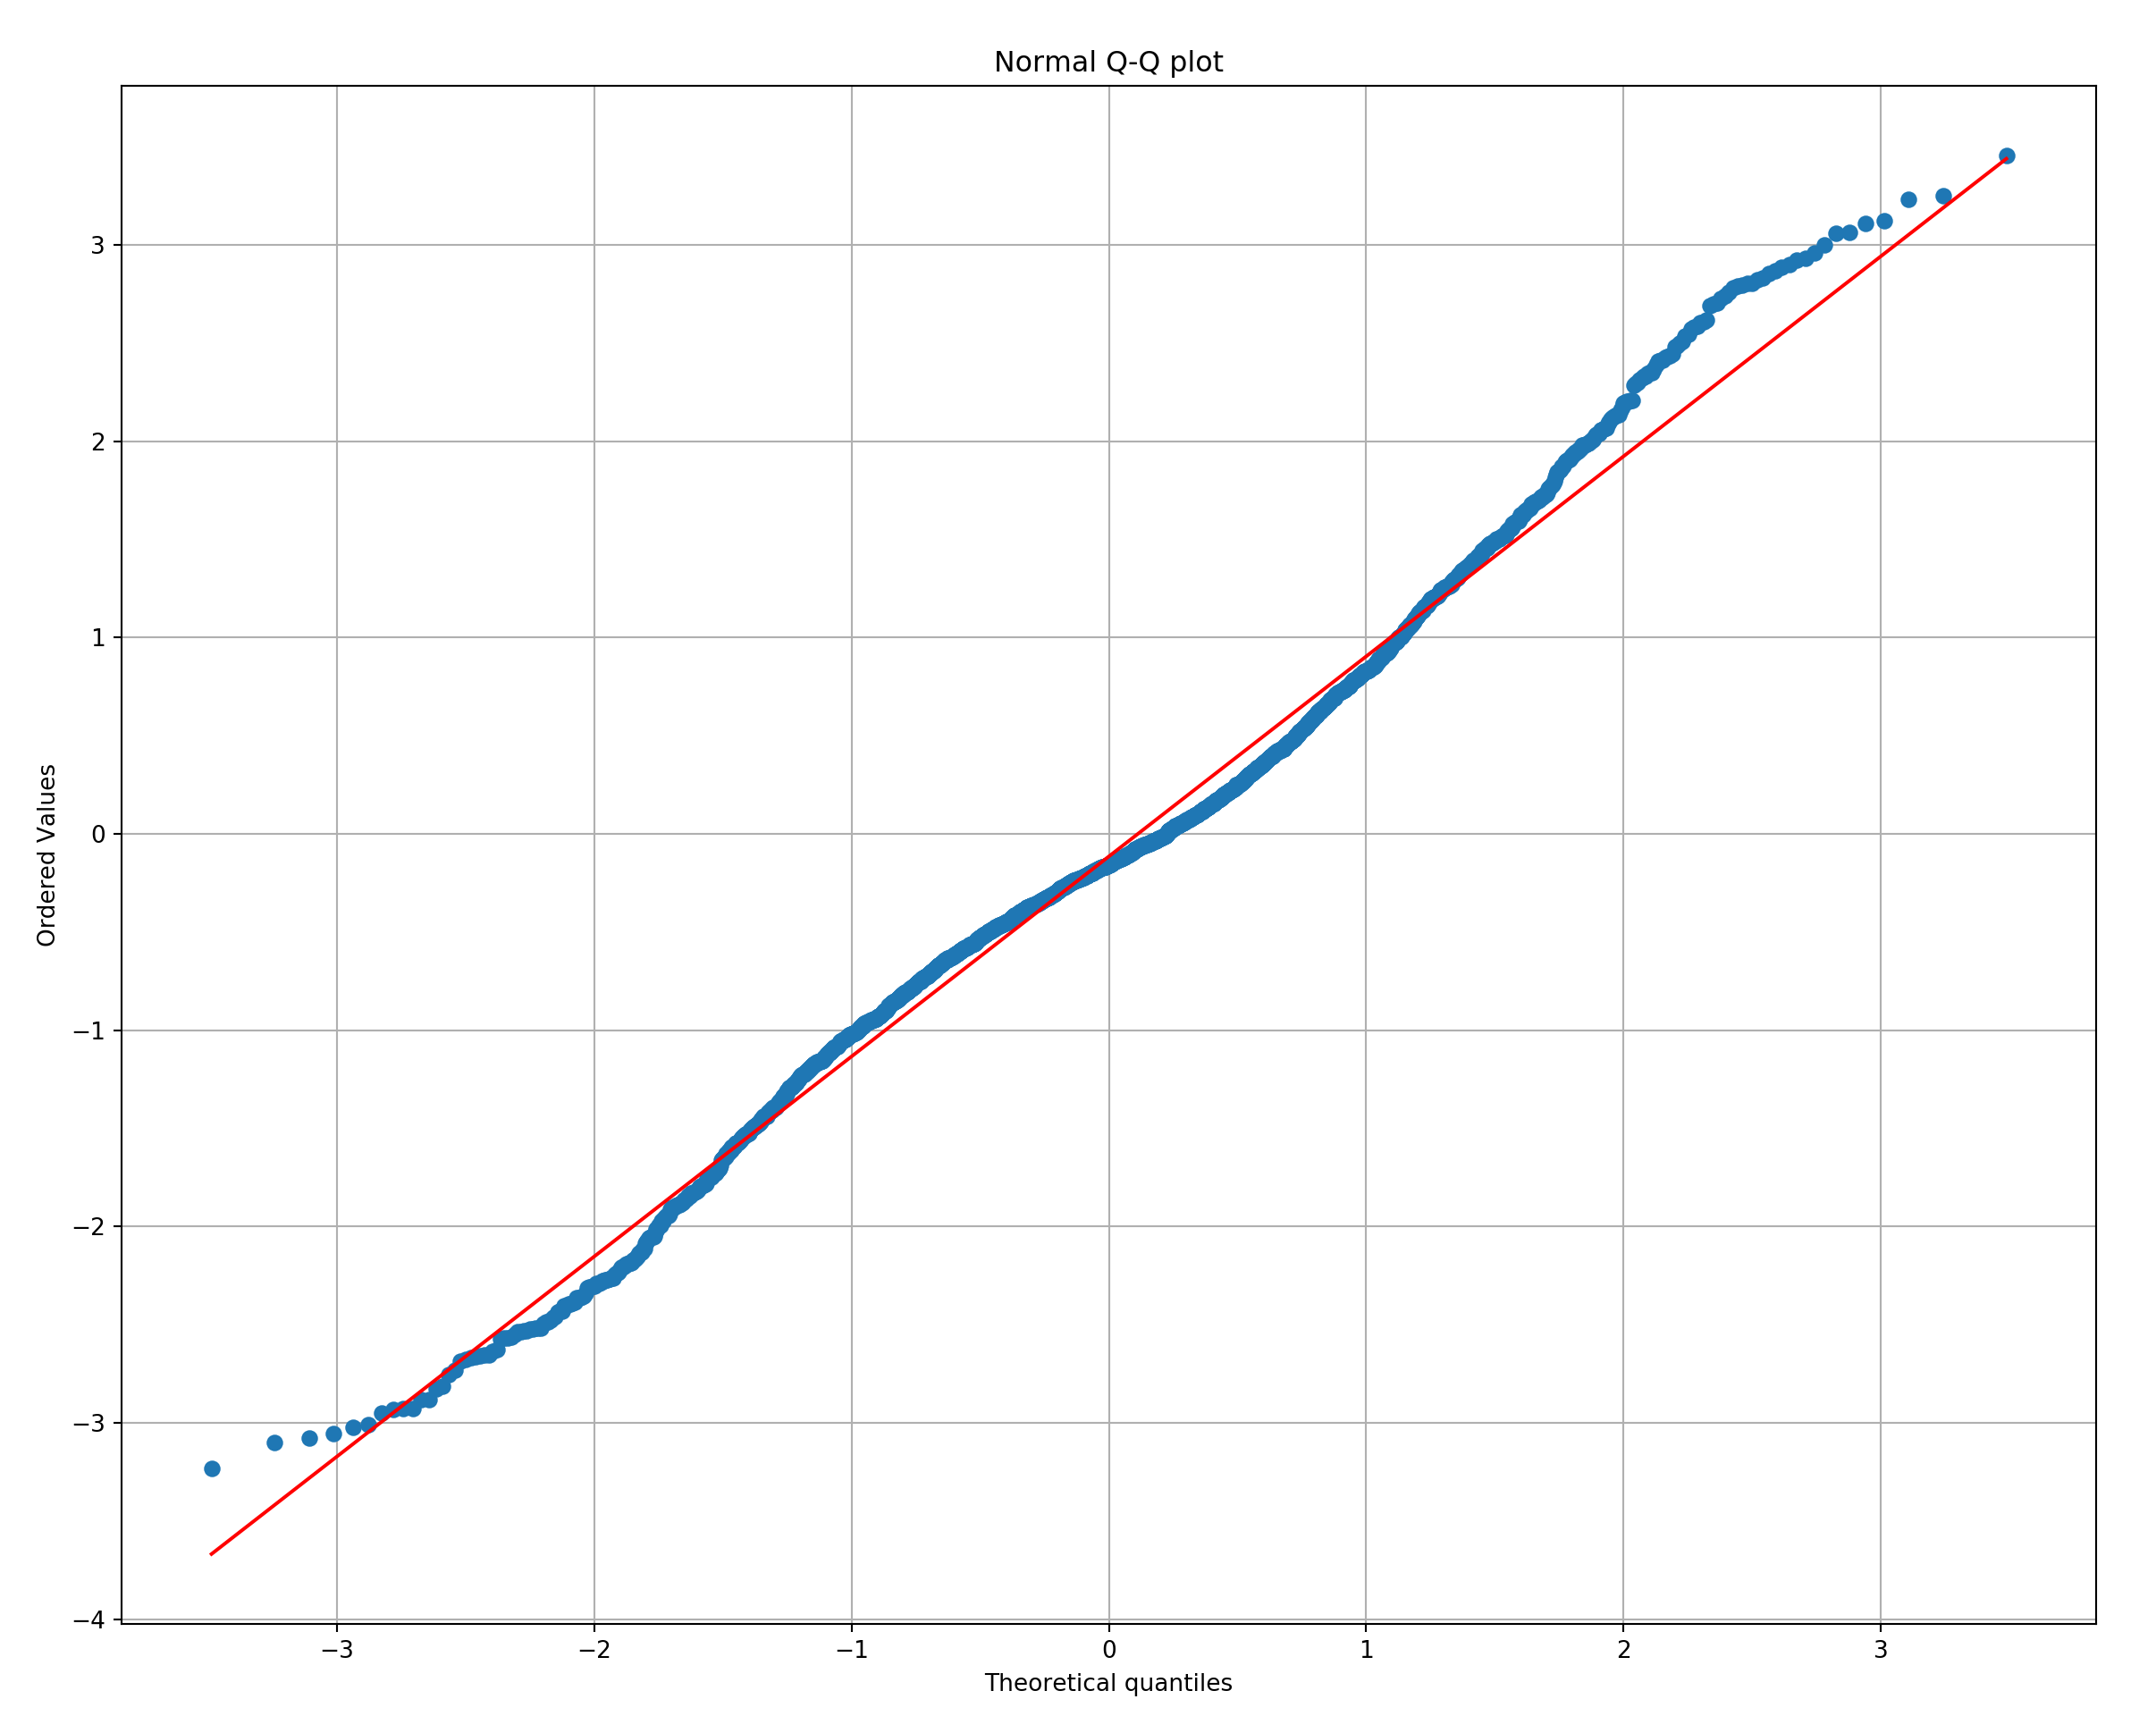
\includegraphics[width=\textwidth]{novas_btc_returns_qqplot.png}
\end{figure}
\end{frame}

%% 5 min bar US Treasury Futures 10 year %%

\begin{frame}
\frametitle{5min Bar 10yr Treasury Futures (1983-2012)}
\begin{figure}[h!]
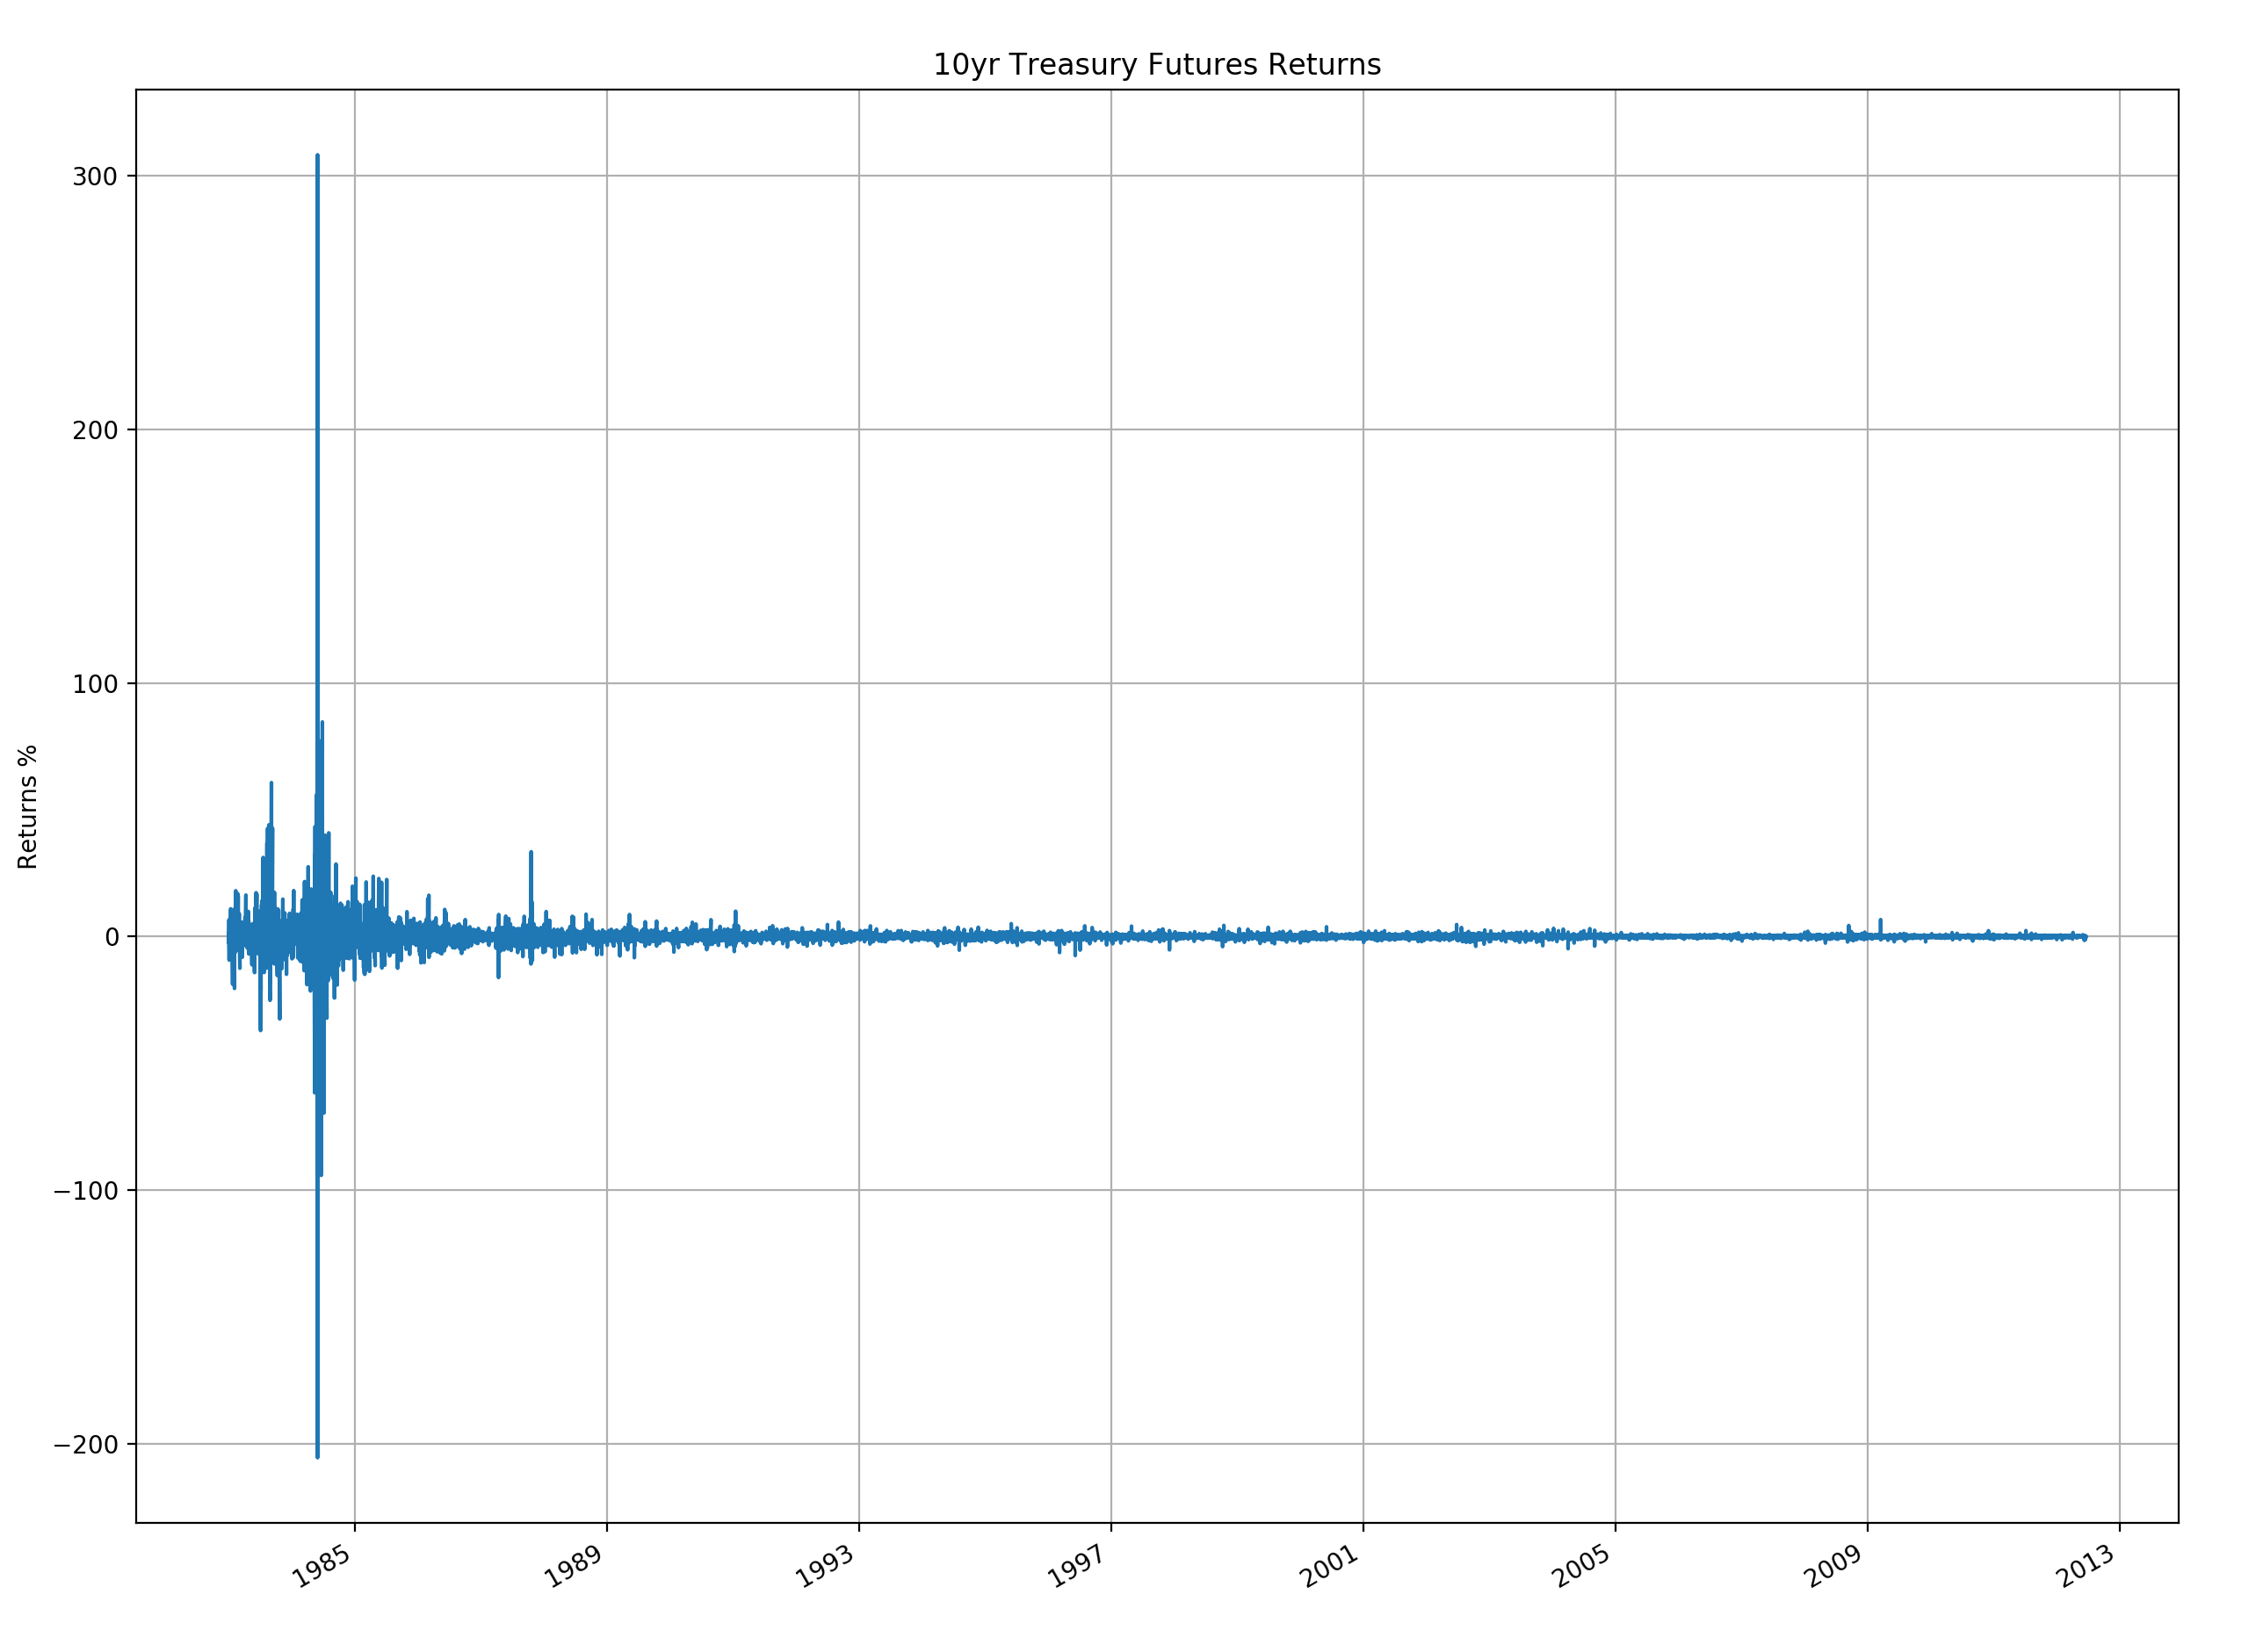
\includegraphics[width=\textwidth]{ty_returns.png}
\end{figure}
\end{frame}

\begin{frame}
\frametitle{5min Bar 10yr Treasury Futures (2010-2012)}
\begin{figure}[h!]
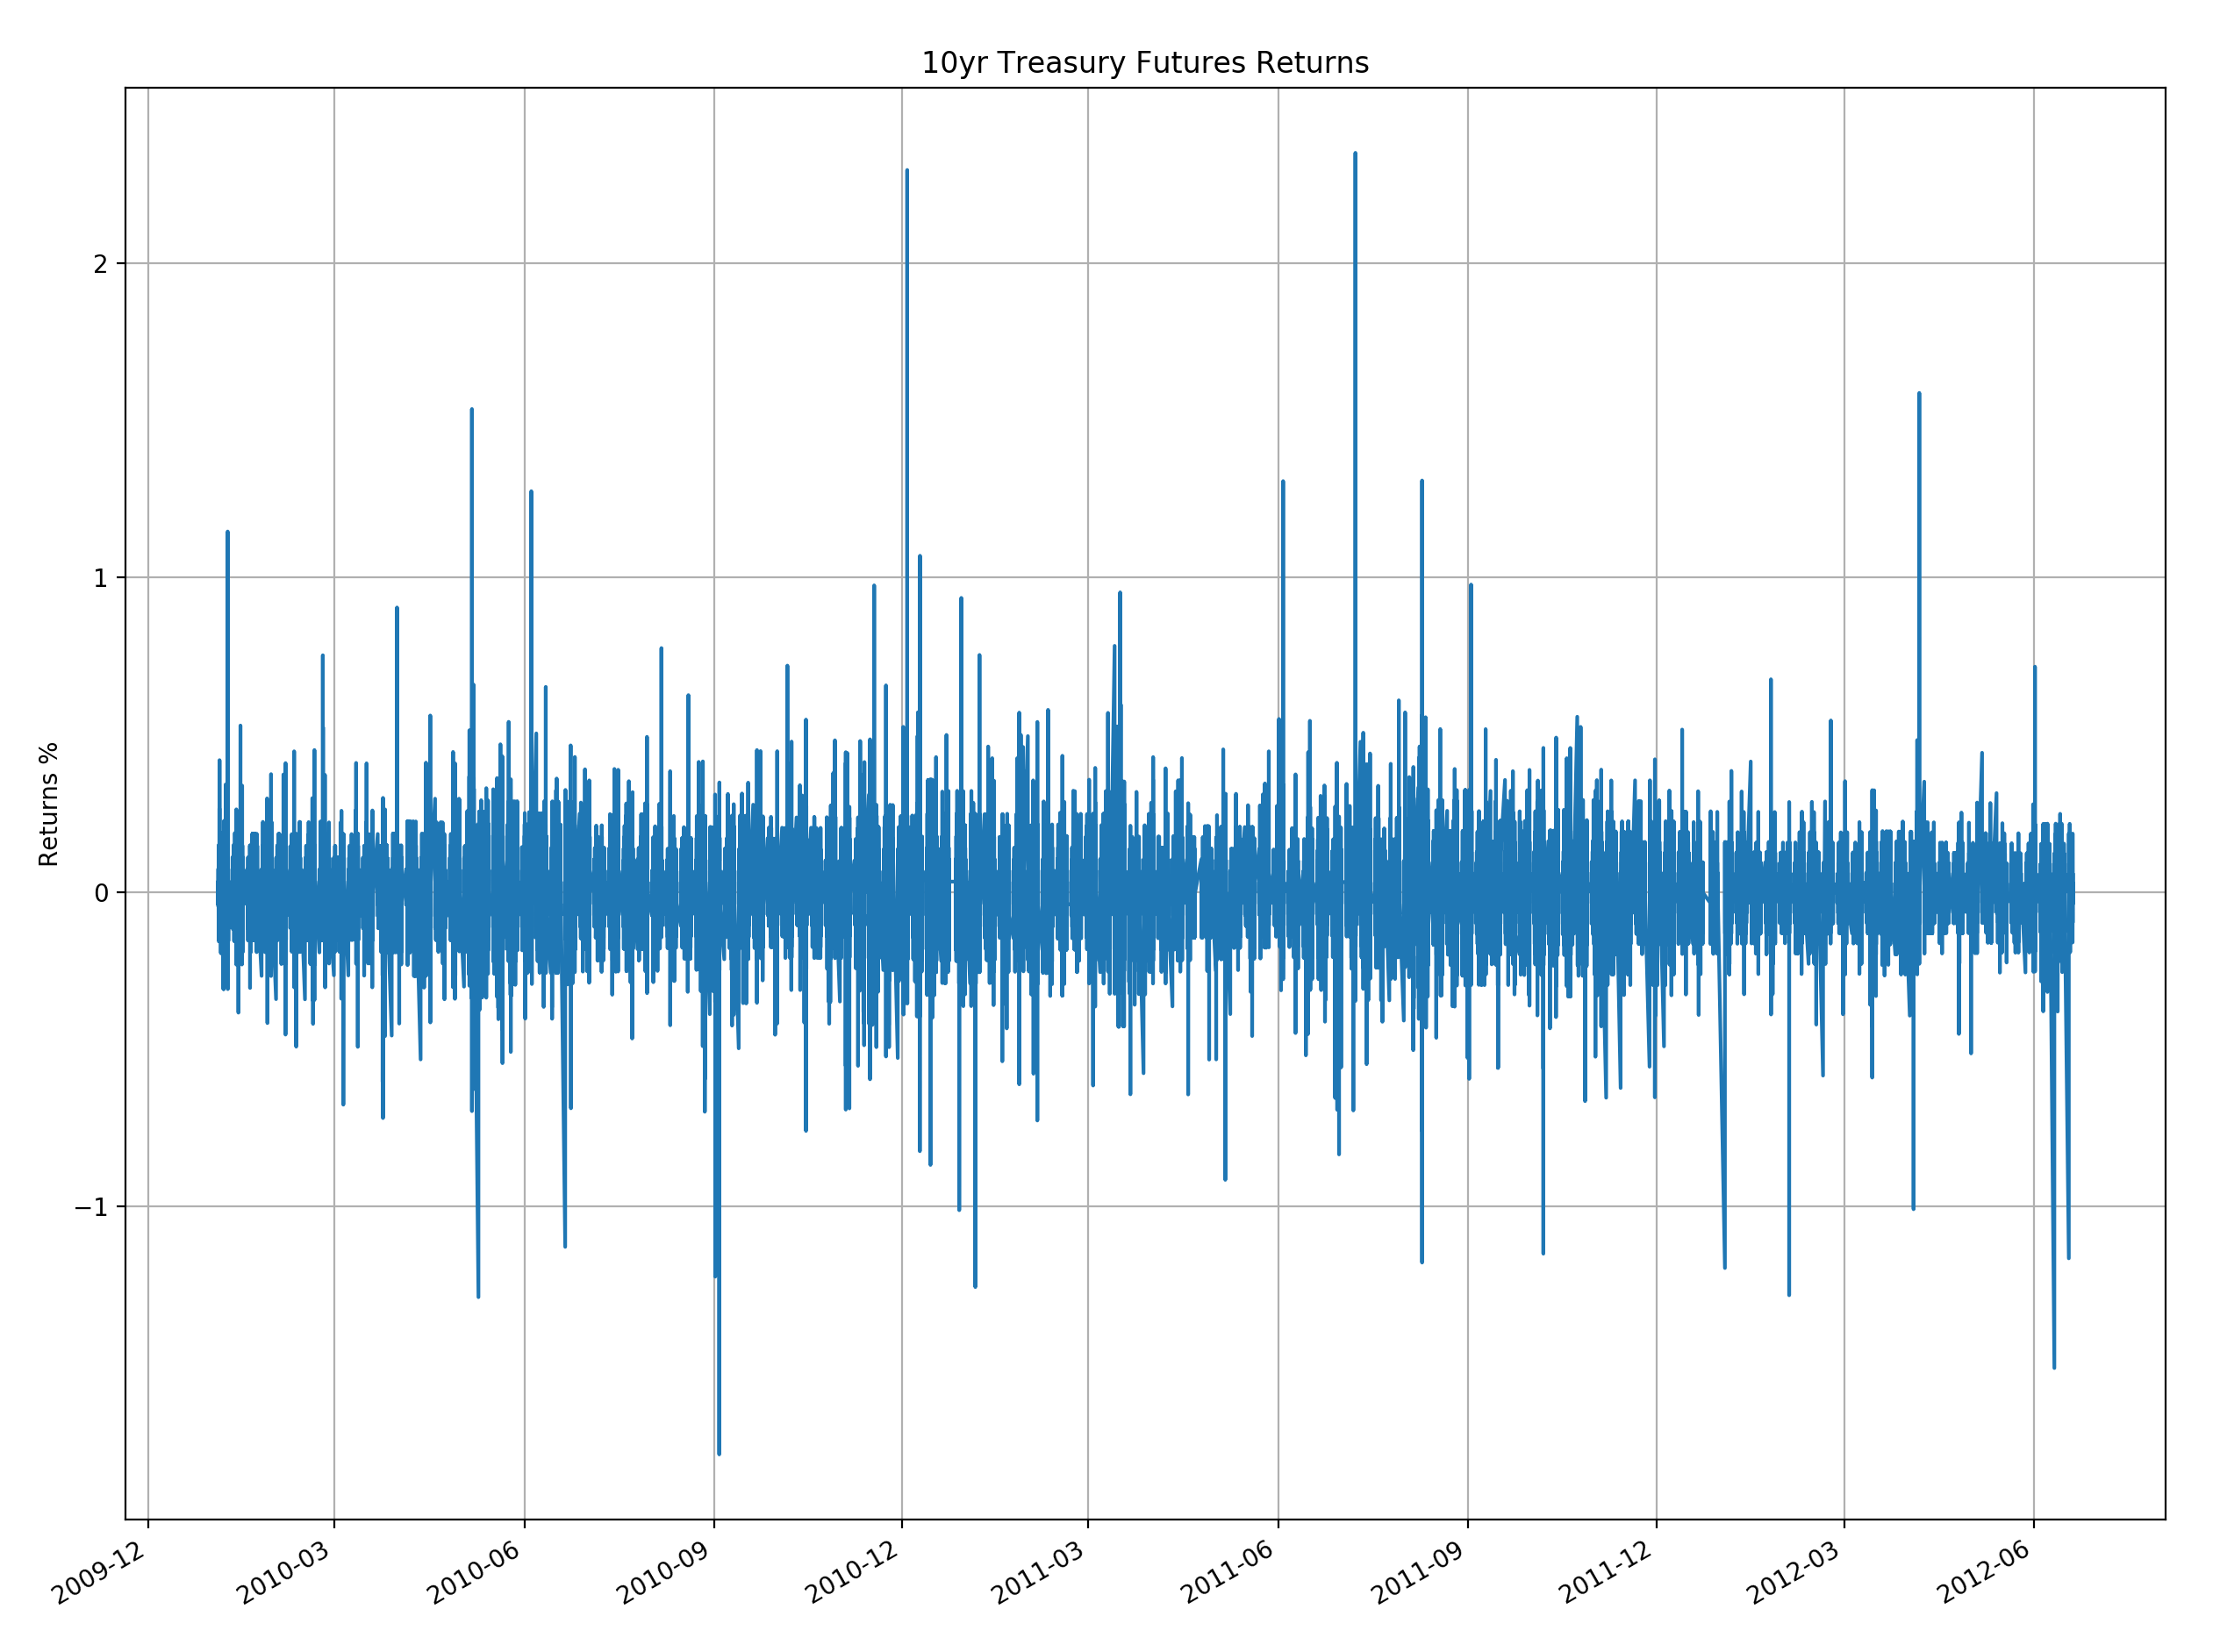
\includegraphics[width=\textwidth]{ty_returns_2010.png}
\end{figure}
\end{frame}

\begin{frame}
\frametitle{5min Bar 10yr Treasury Futures (2010-2012)}
\begin{figure}[h!]
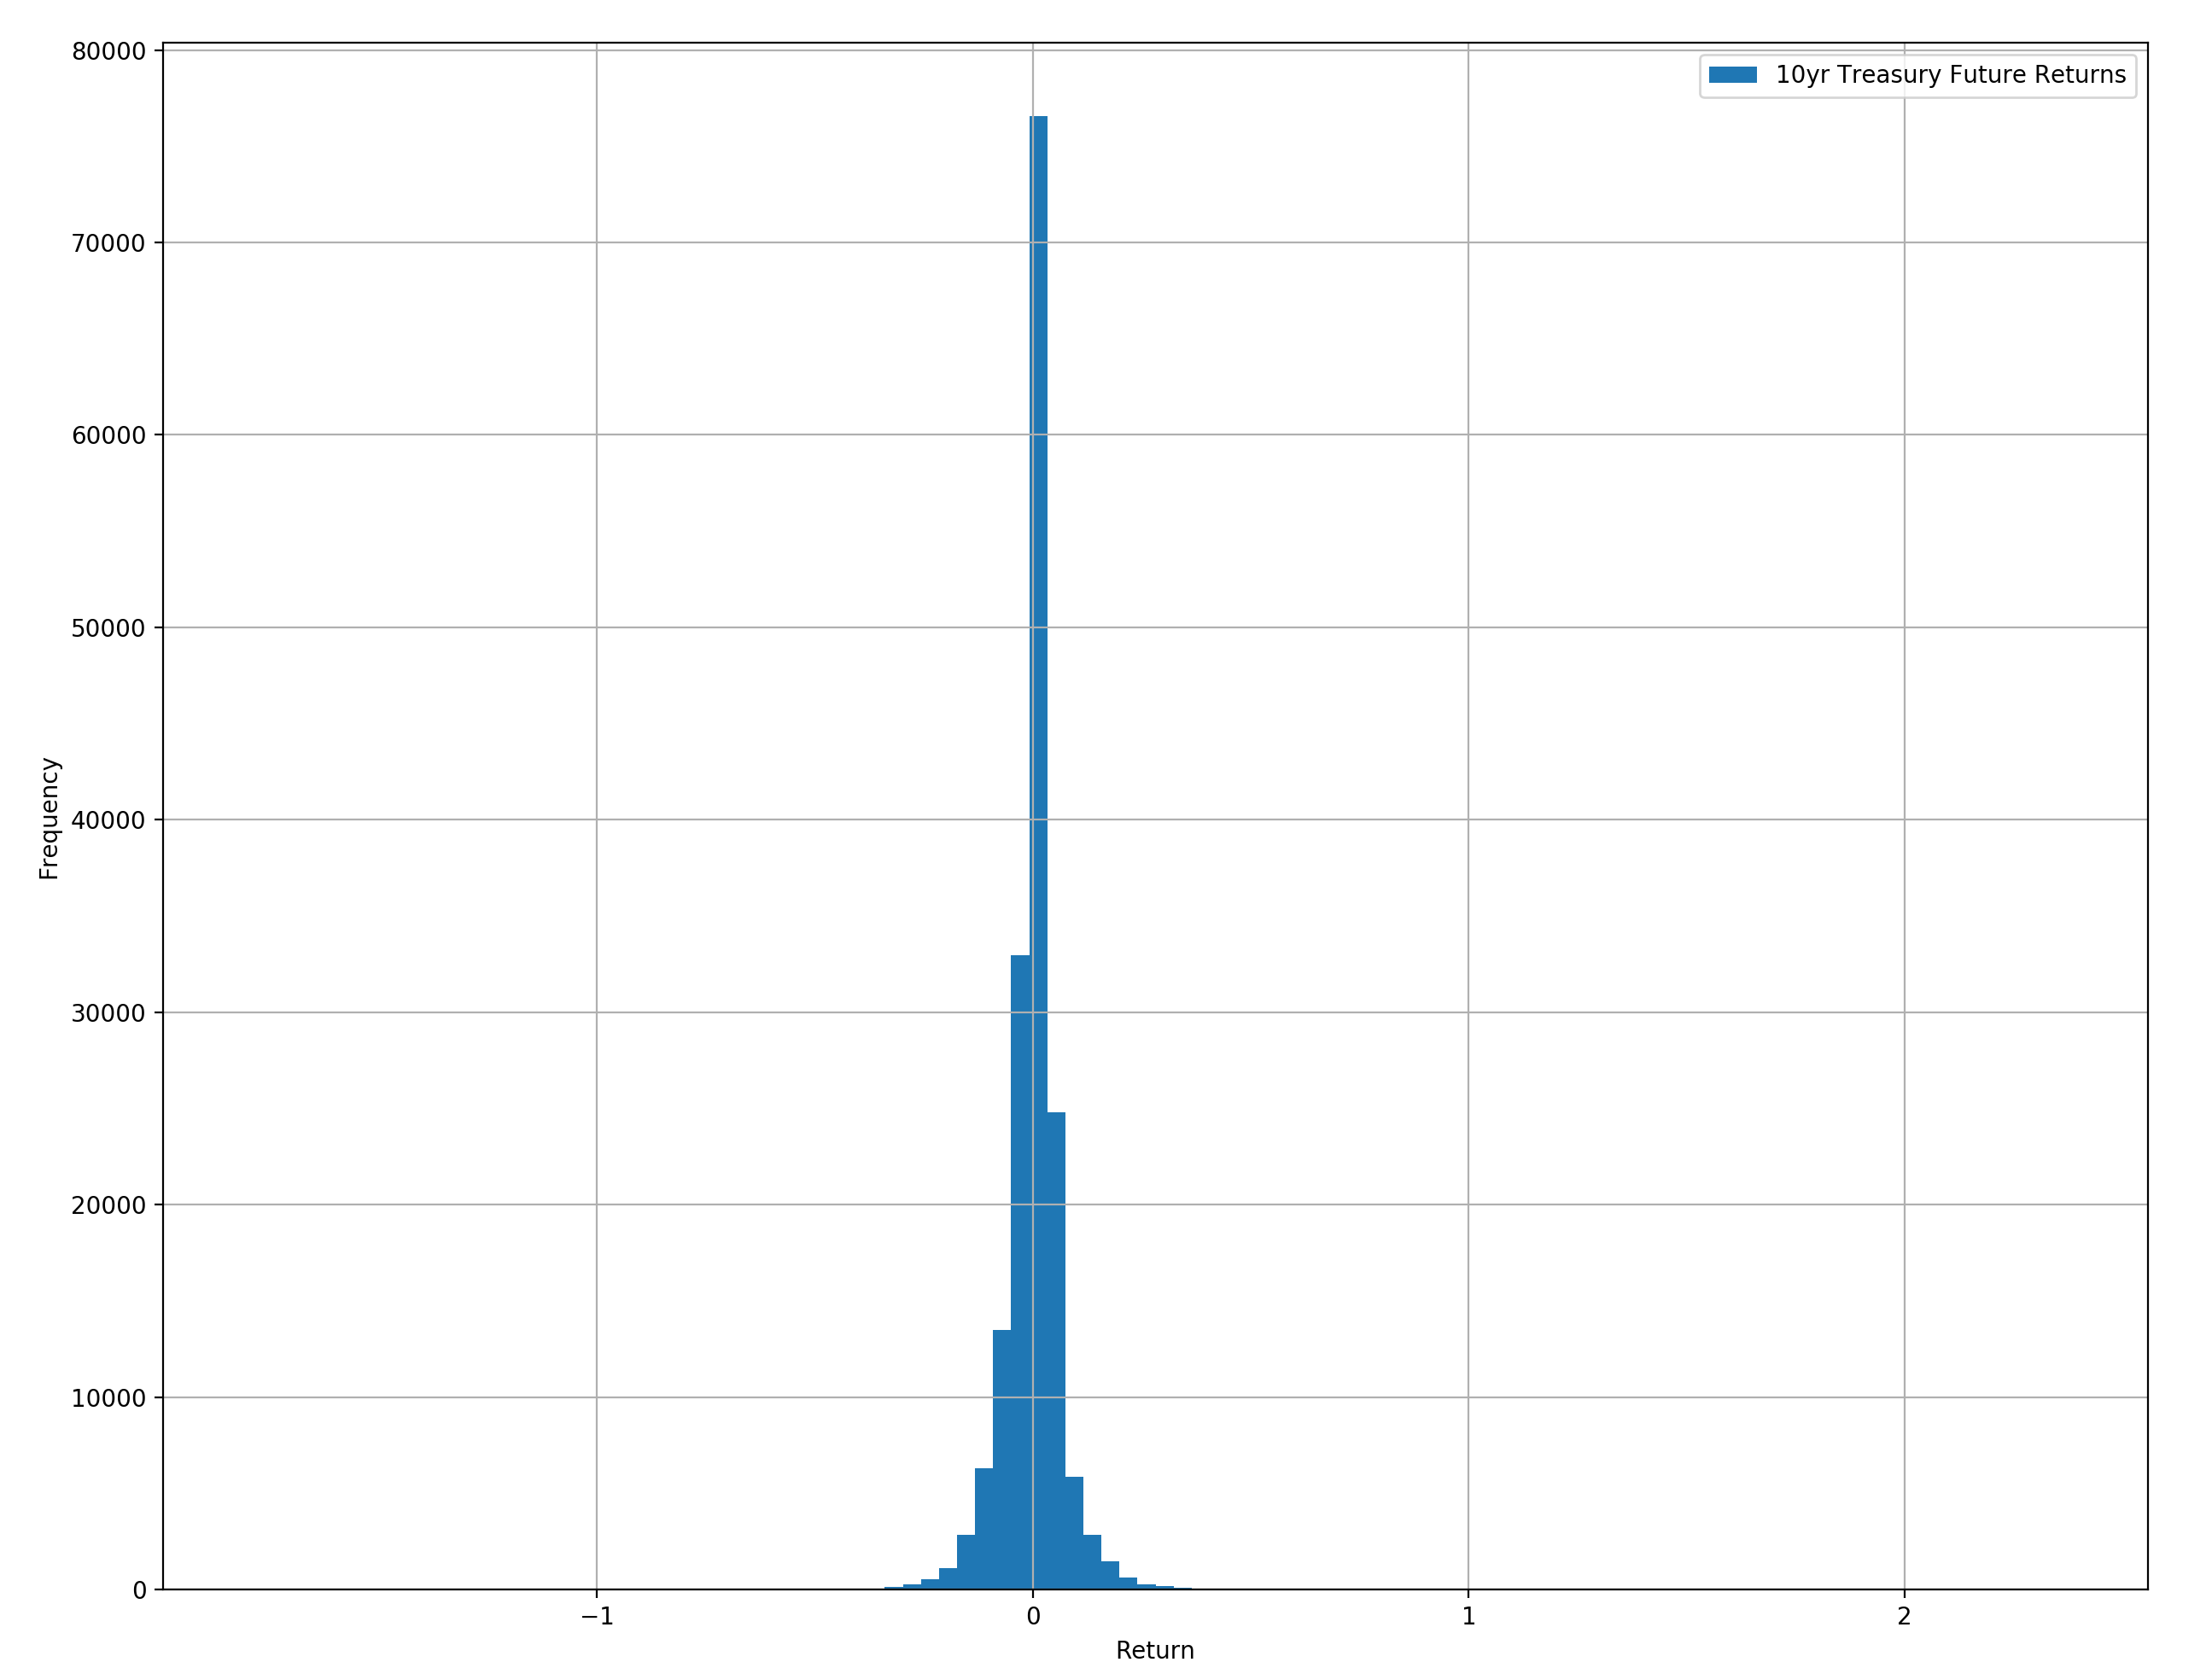
\includegraphics[width=\textwidth]{ty_returns_2010_hist.png}
\end{figure}
\end{frame}

\begin{frame}
\frametitle{5min Bar 10yr Treasury Futures (2010-2012)}
\begin{figure}[h!]
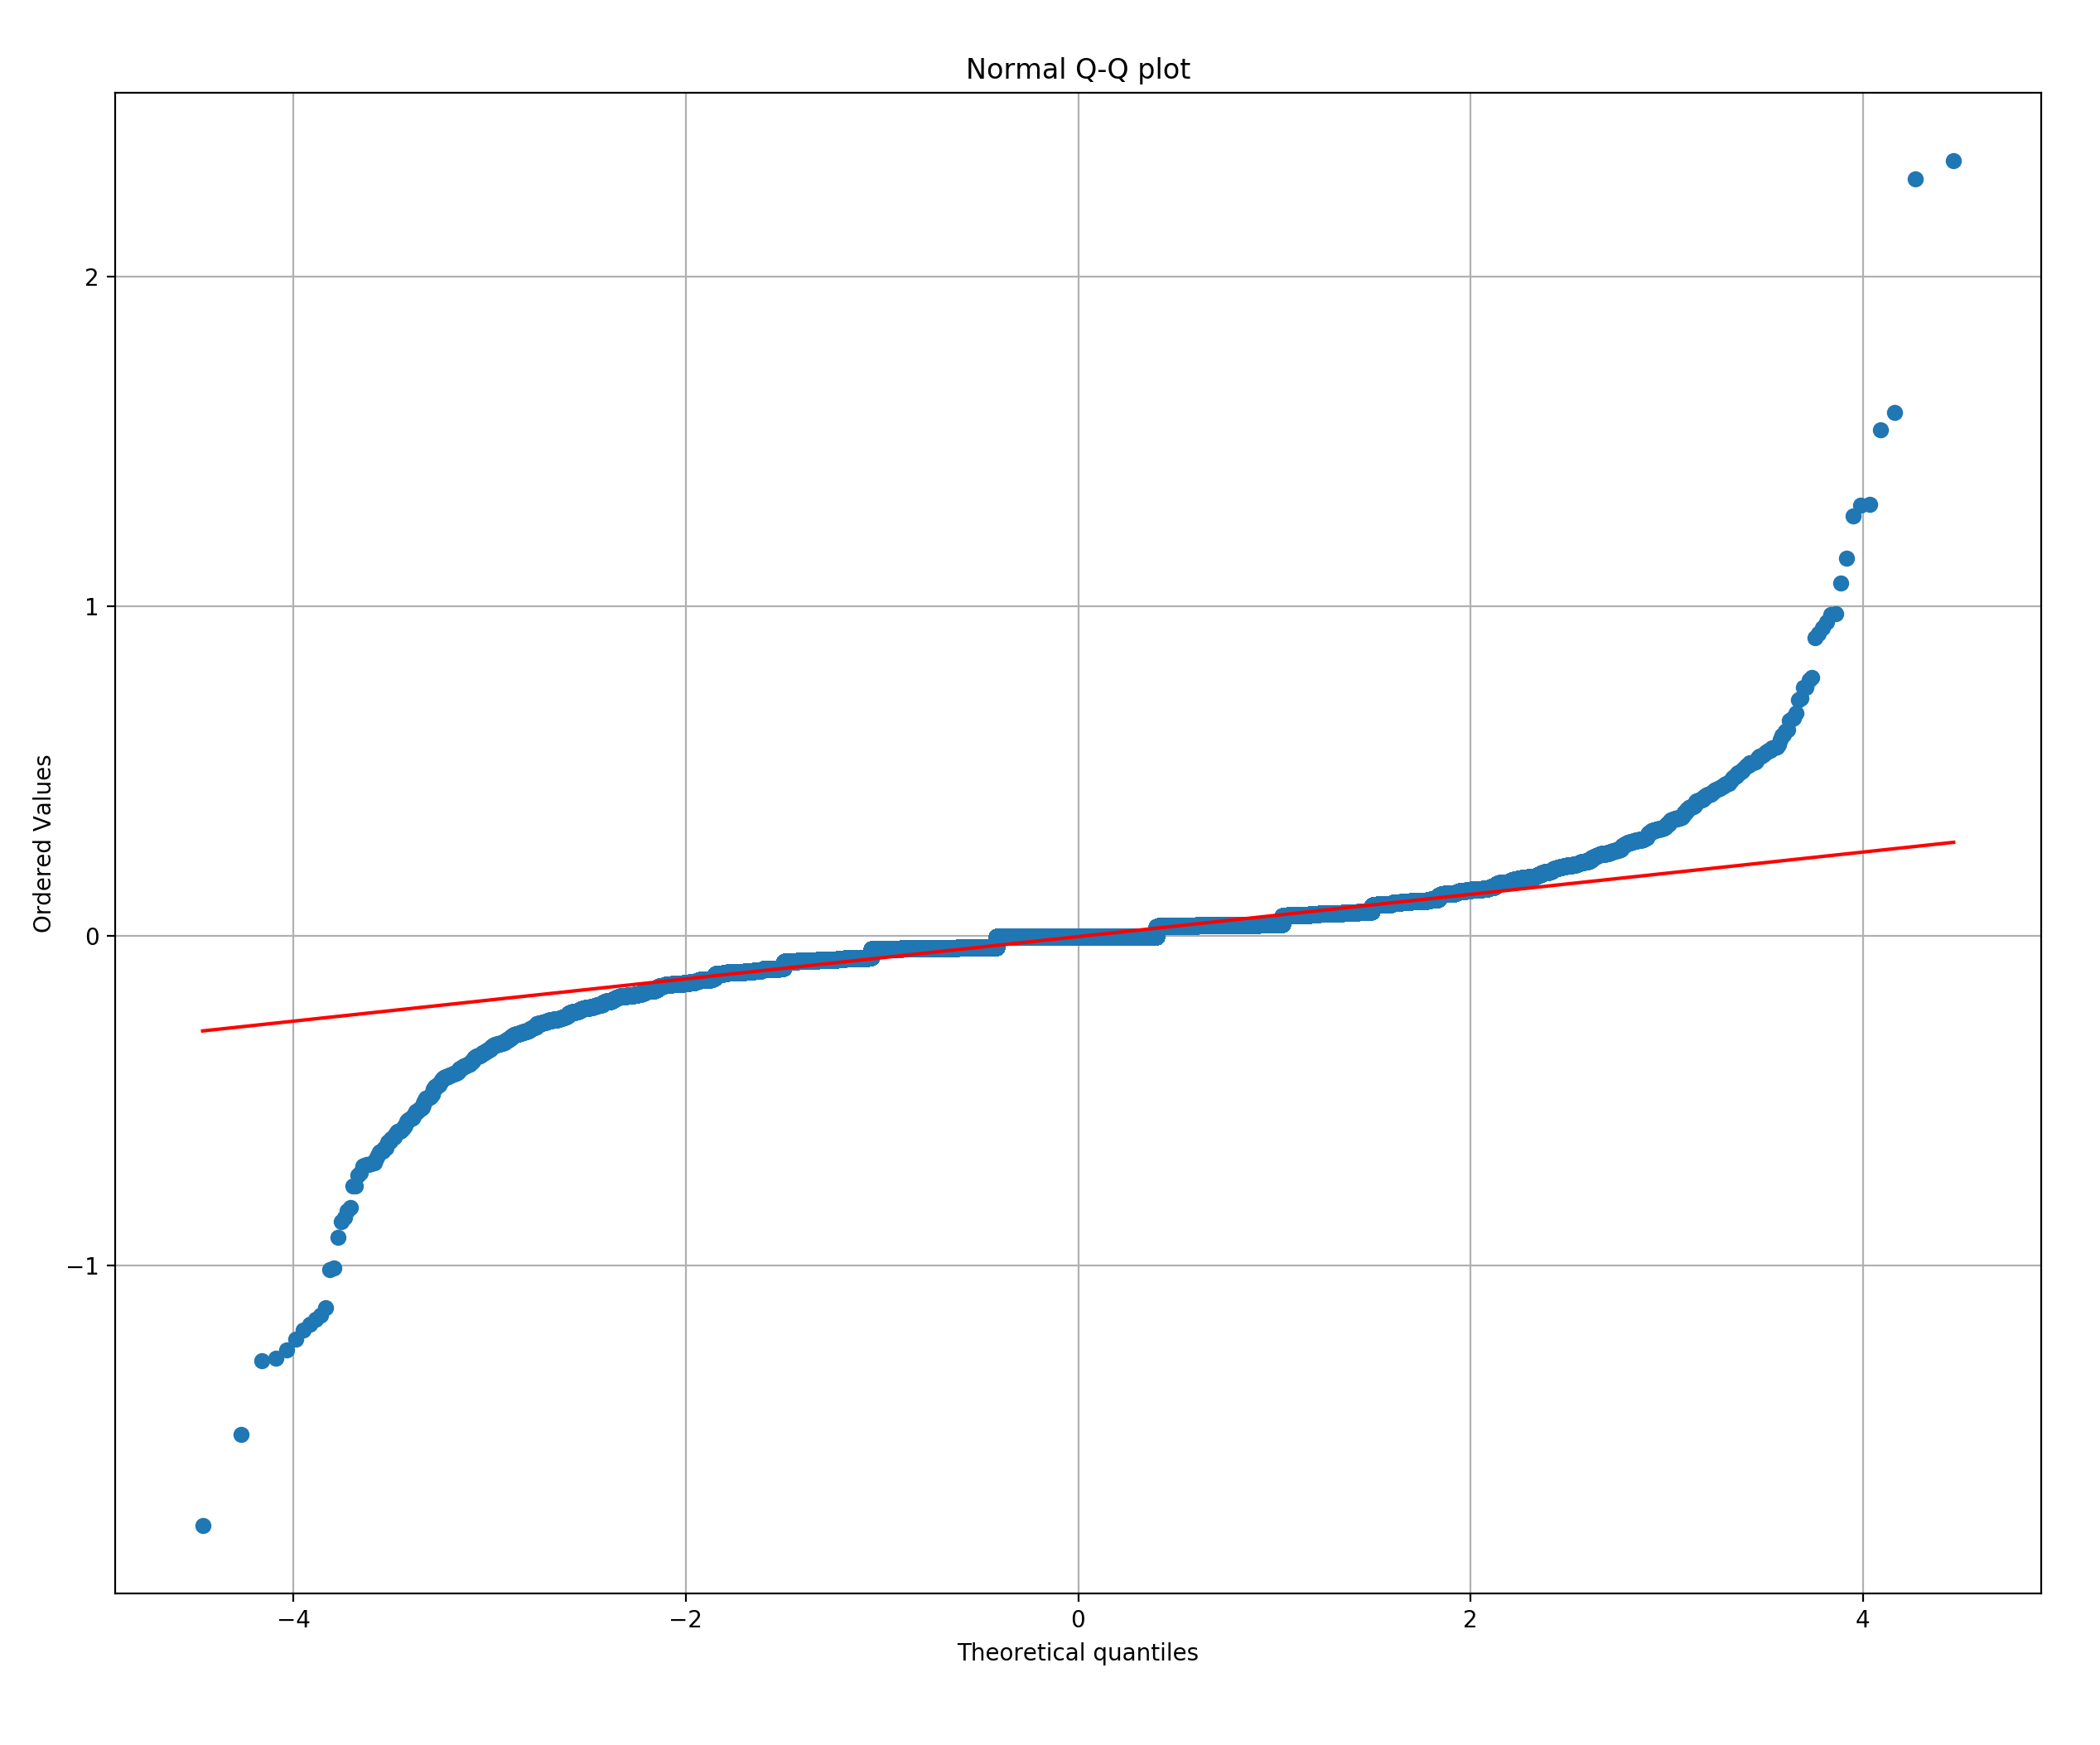
\includegraphics[width=\textwidth]{ty_returns_2010_qqplot.png}
\end{figure}
\end{frame}

\begin{frame}
\frametitle{NoVaS 10yr Treasury Futures (1983-2012) (p=12)}
\begin{figure}[h!]
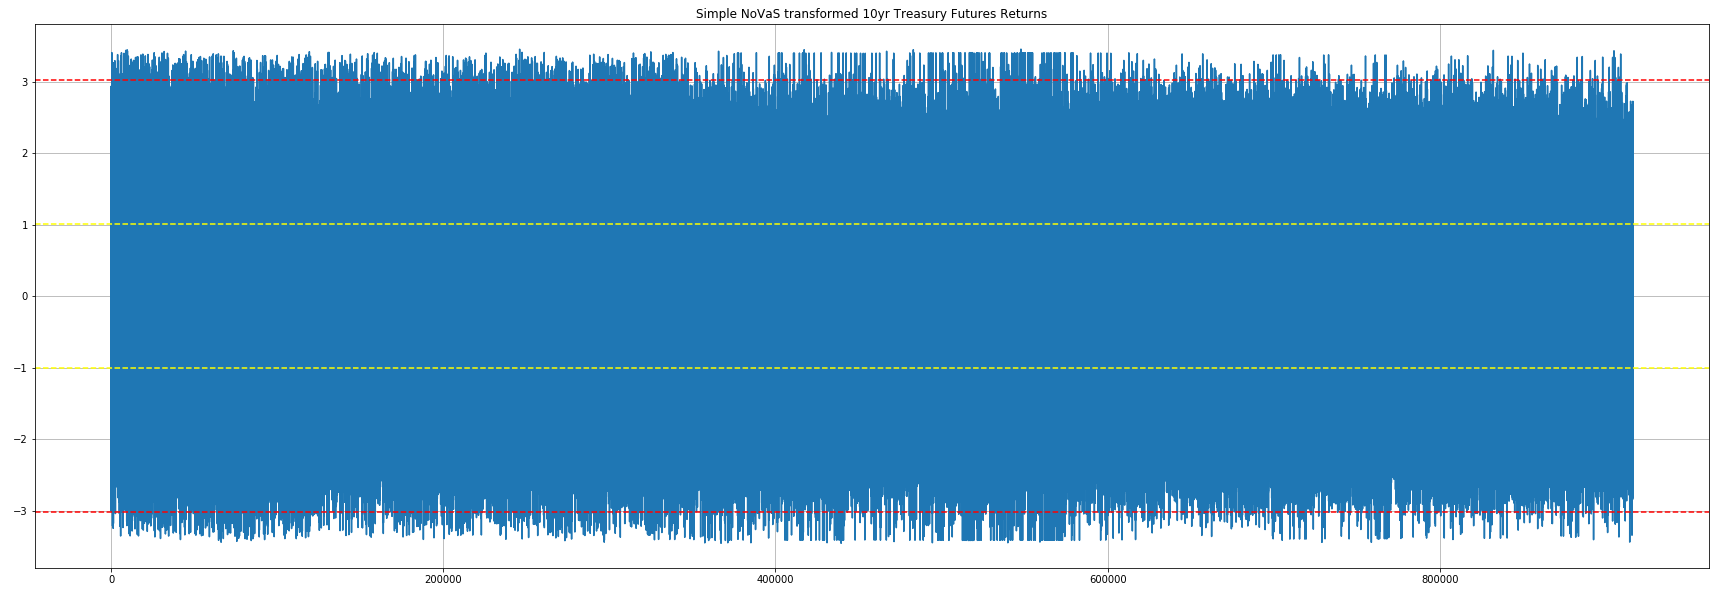
\includegraphics[width=\textwidth]{novas_ty_returns.png}
\end{figure}
\end{frame}

\begin{frame}
\frametitle{NoVaS 10yr Treasury Futures (2010-2012) (p=12)}
\begin{figure}[h!]
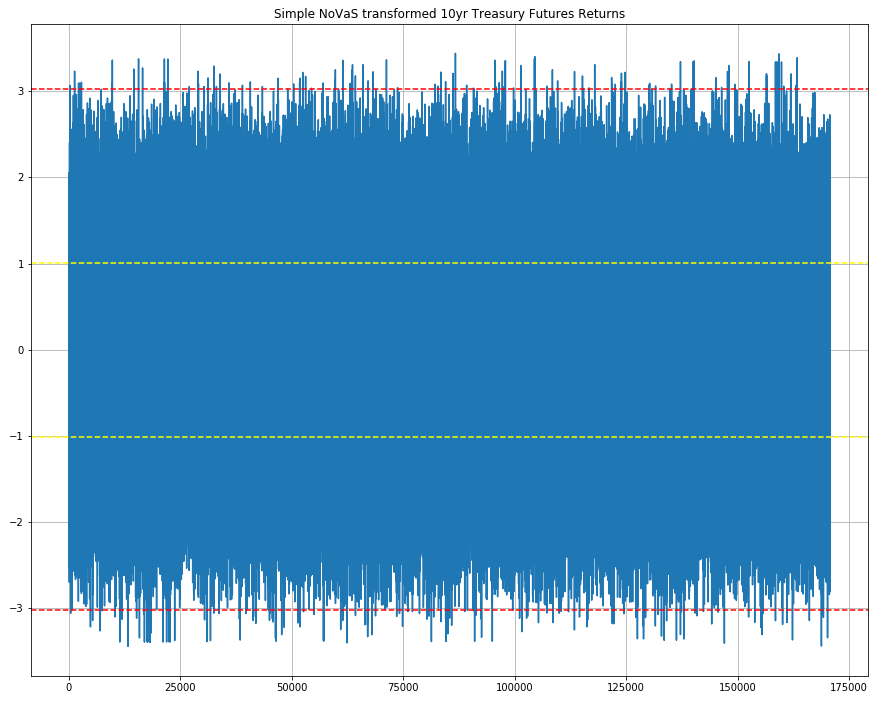
\includegraphics[width=\textwidth]{novas_ty_returns_2010.png}
\end{figure}
\end{frame}

\begin{frame}
\frametitle{NoVaS 10yr Treasury Futures (2010-2012) (p=12)}
\begin{figure}[h!]
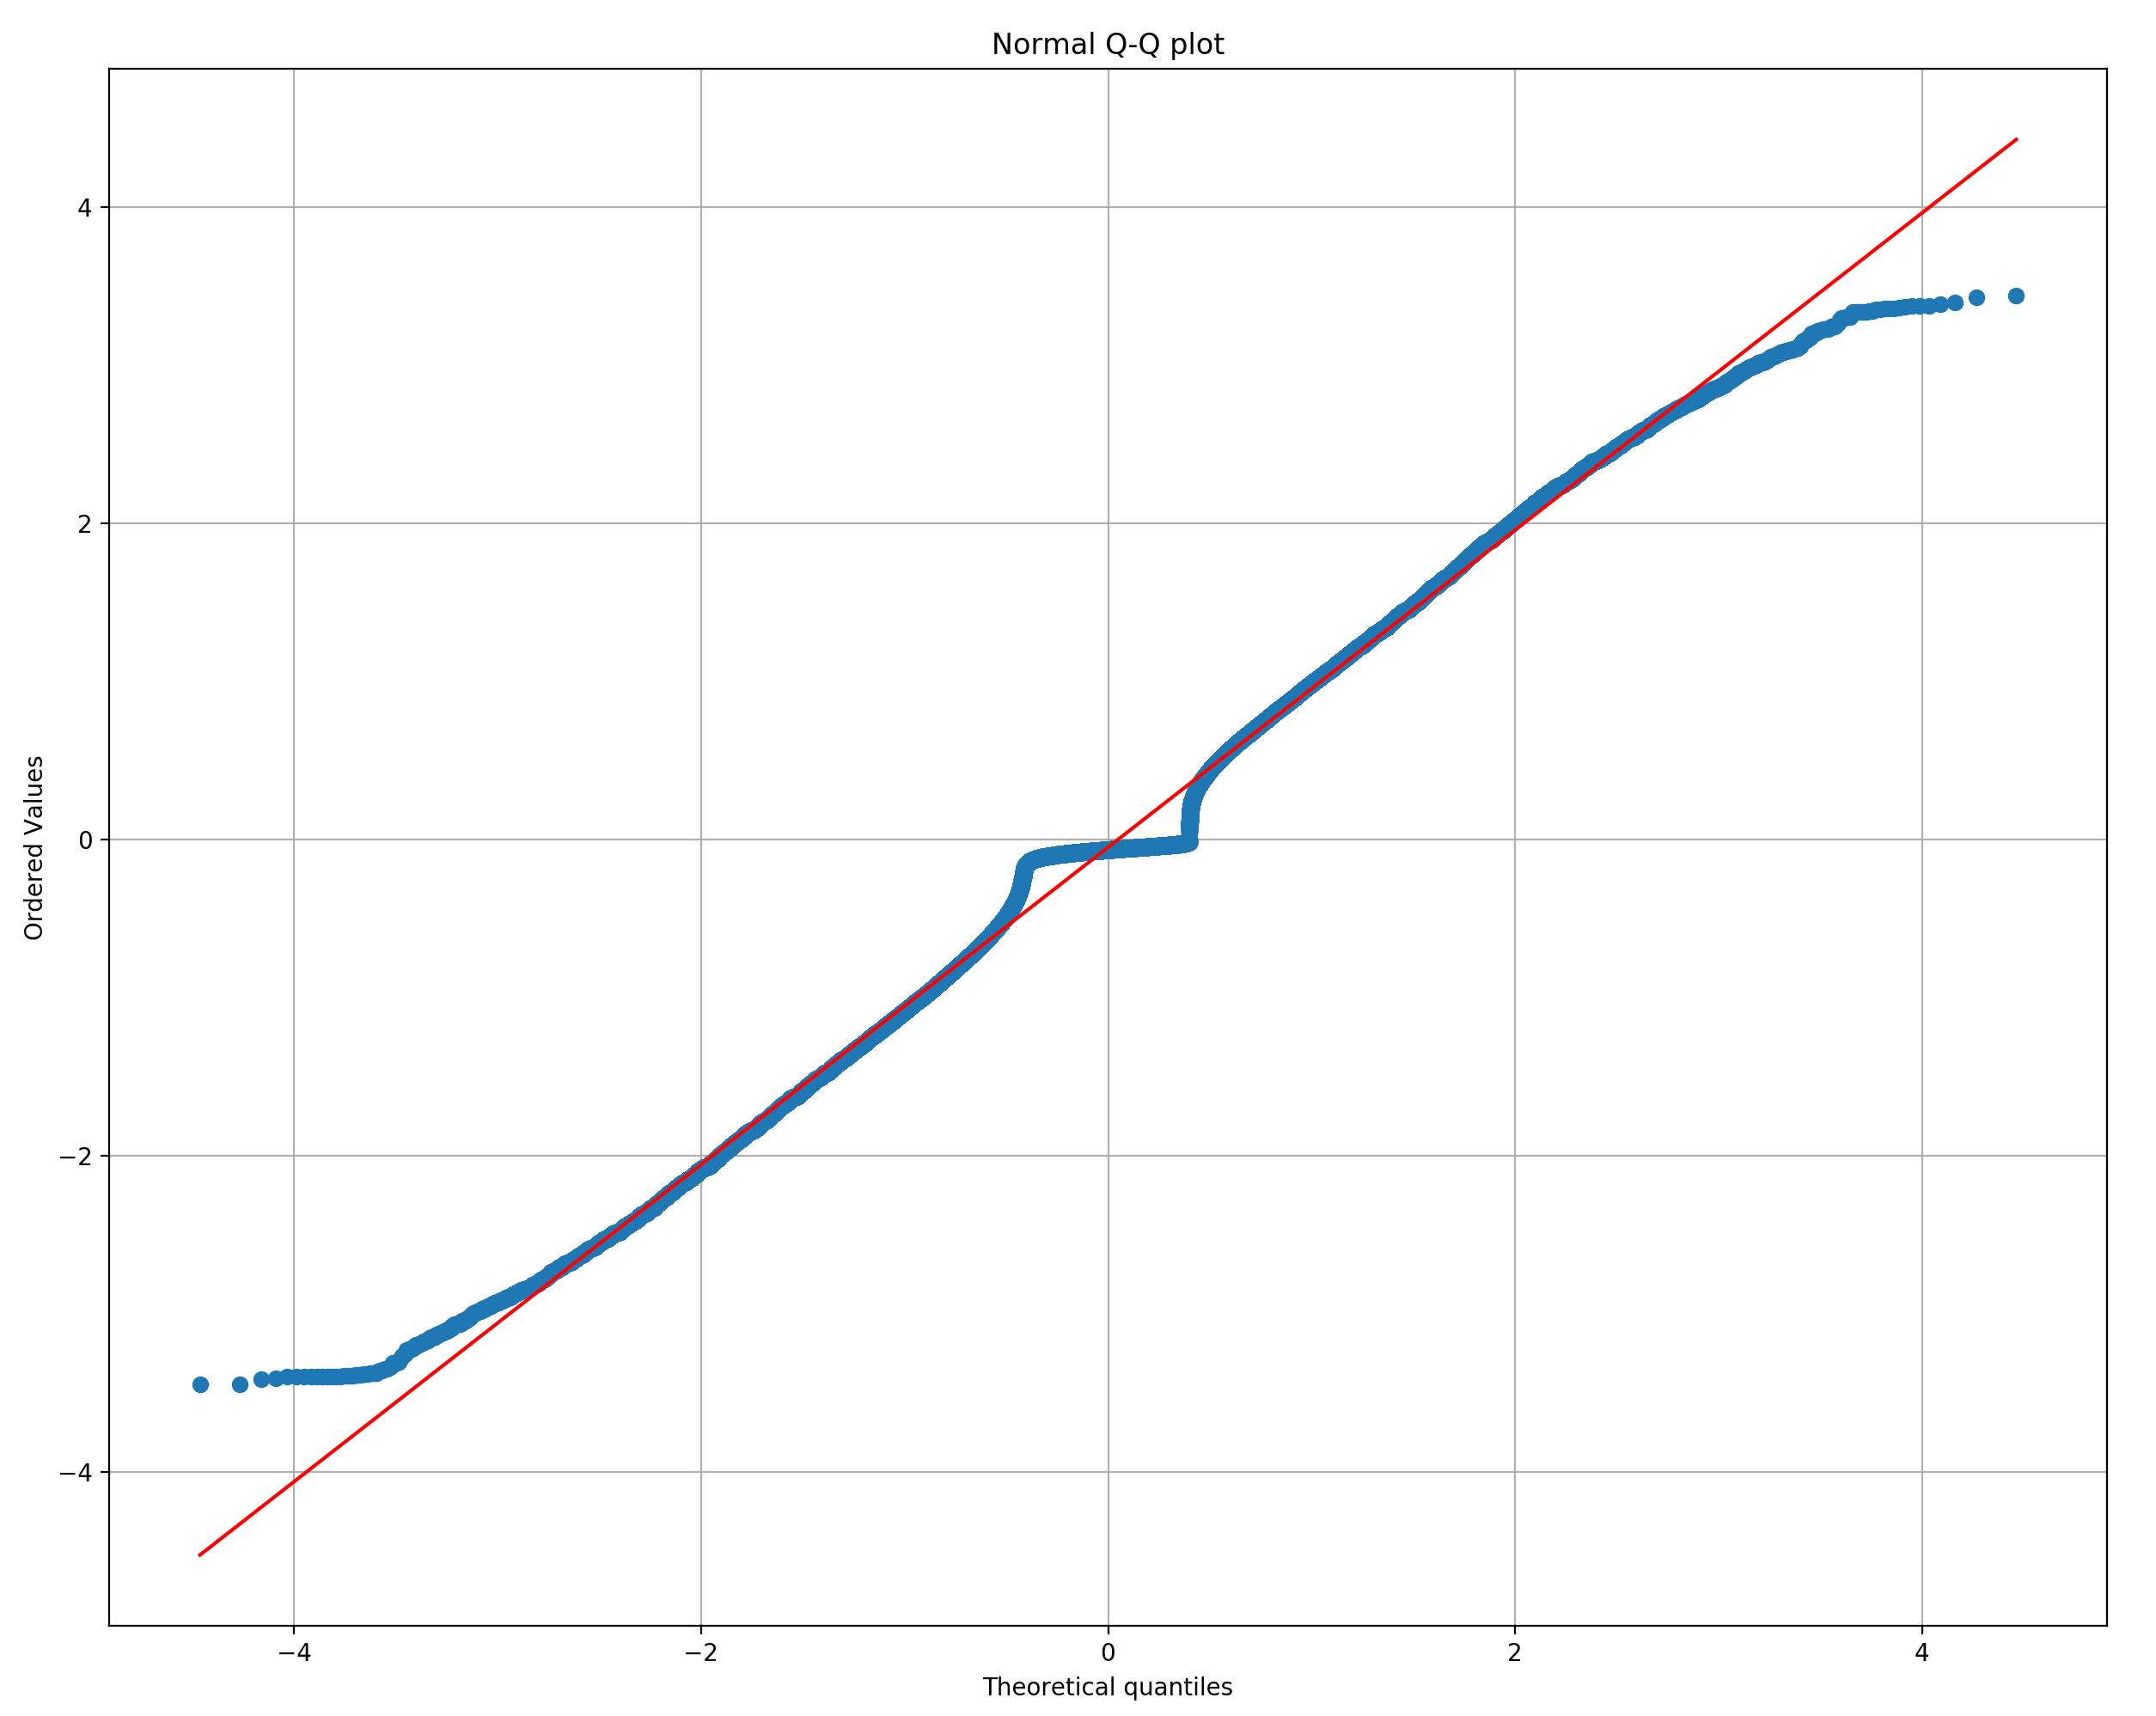
\includegraphics[width=\textwidth]{novas_ty_returns_2010_qqplot.png}
\end{figure}
\end{frame}


% THIS IS NOT TRUE, SIMPLE NOVAS SEEMS VERY ROBUST AGAINST
% DIFFERENT SUBSETS OF THE DATA

%\begin{frame}
%\frametitle{S&P500 not perfect tranform with NoVaS}
%Simply show an imperfect transformation to make the point that financial time series over long periods are not necessary stationary (only locally stationary) and thus we should use time-varying versions of NoVaS where the window size isn't too big.
%\end{frame}


\section{Volatility Prediction}

\begin{frame}
\frametitle{Outline}
\tableofcontents[currentsection]
\end{frame}

\begin{frame}
\frametitle{Volatility Prediction}

\begin{itemize}
\item{Forecasts of volatility are important when assessing and managing the risks of portfolios}
\vspace{3pt}
\item{We focus on the problem of one-step ahead $X_{t+1}$ prediction based on the observed past}
\vspace{3pt}
\item{For our purposes, volatility prediction = predicting $X_{t+1}^2$}
\vspace{3pt}
\item{Even though $X_{t+1}^2$ is a noisy proxy for $\mathbb{E}(X_{t+1}^2|\mathfrak{F_n})$, we'll see that in under some conditions NoVaS allows us to predict the latter}
\vspace{3pt}
%\item{$X_{t}^2$ has the theoretical advantage that optimal forecasts can also be optimal forecasts for $\sigma^2$, however we'll show that this condition isn't particularly relevant}
\item{Assuming more realistically that financial returns are locally stationary, we use a rolling window size of 250 days to calculate our forecasts}
\end{itemize}
\end{frame}

\begin{frame}
\frametitle{Which Loss Function? $L_1$ or $L_2$?}
\begin{itemize}
\item{To assess the accuracy of forecasts, we need to decide on a loss function to use}
\vspace{3pt}
\item{The MSE is most commonly used, however note that $\mathbb{E}(Y_{n+1}^{2}-\widehat{Y_{n+1}^2})^2$ is essentially a fourth moment}
\vspace{3pt}
\item{Thus the unconditional MSE is infinite if the returns process has infinite kurtosis!}
\vspace{3pt}
\item{We find that this indeed the case and so focus on the Mean Absolute Deviation (MAD) loss function}
\vspace{3pt}
\item{Under the objective of $L_1$-optimal prediction, the optimal predictor is $Median(X_{n+1}^2|\mathfrak{F_n})$}
\end{itemize}
\end{frame}

\begin{frame}
\frametitle{Empirical Kurtosis Plot S\&P500}
\begin{figure}[h!]
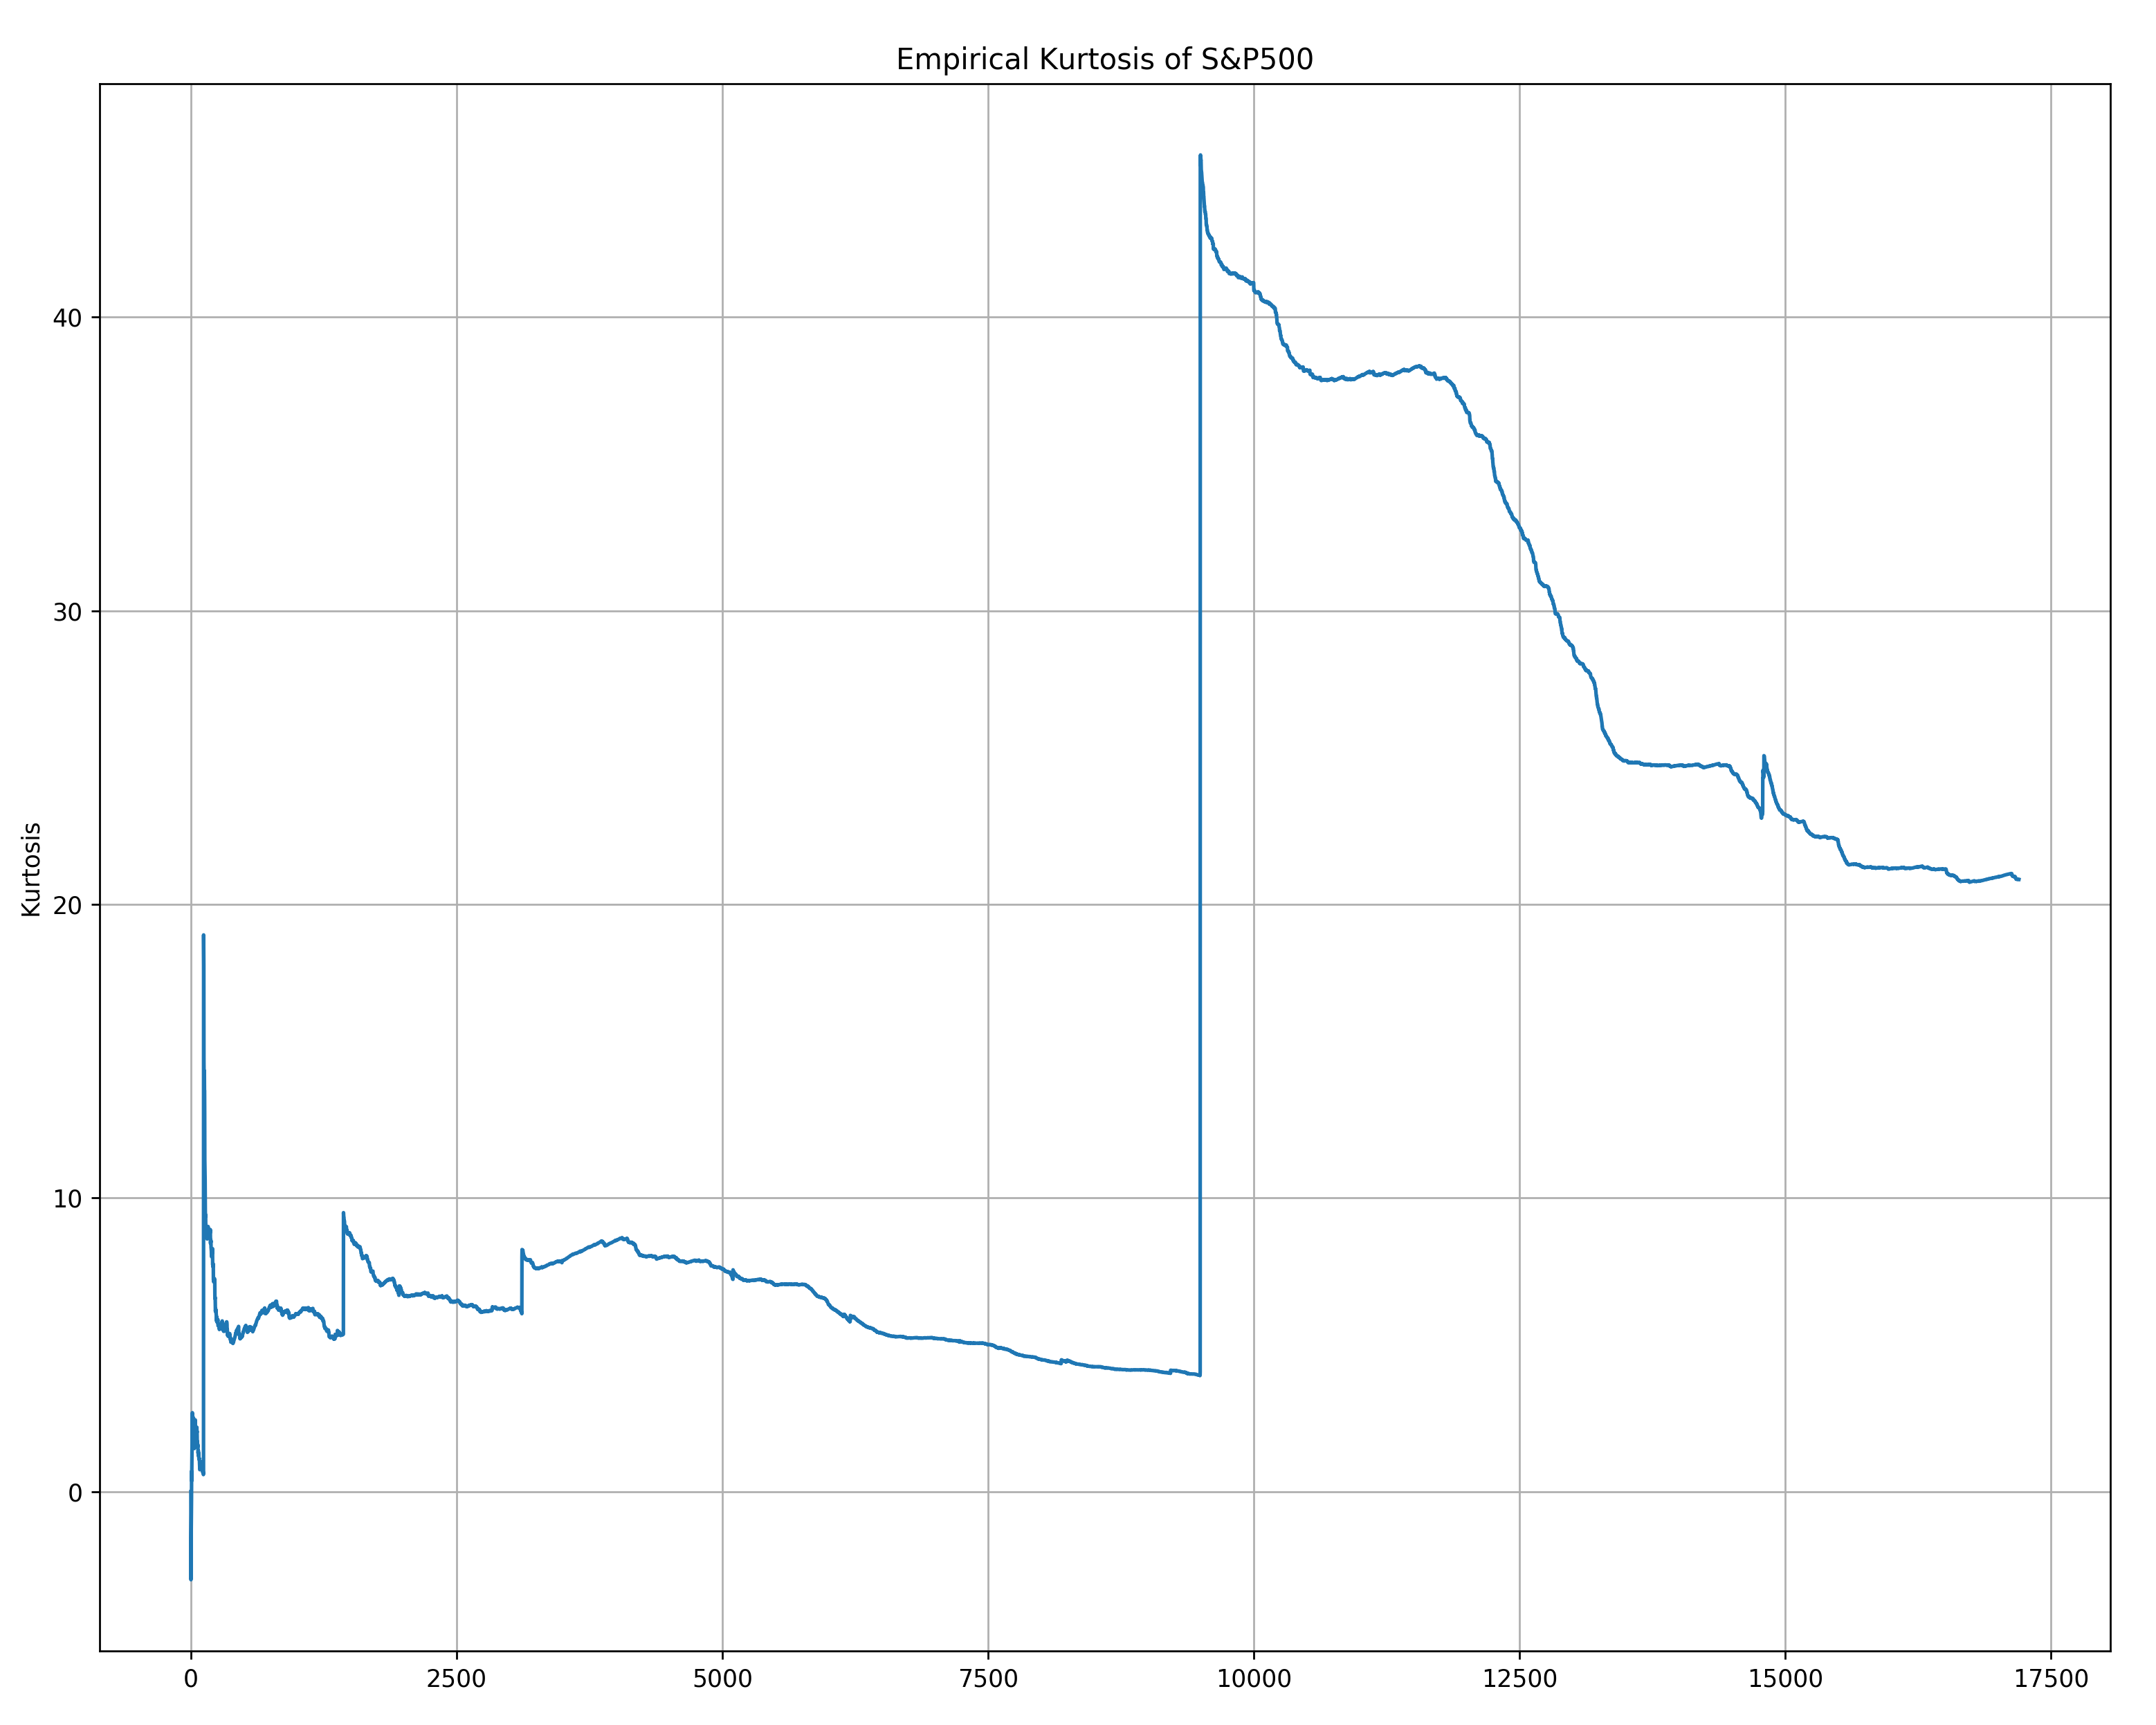
\includegraphics[width=\textwidth]{sp500_returns_kurtosis.png}
\end{figure}
\end{frame}

\begin{frame}
\frametitle{Empirical Kurtosis Plot BTC}
\begin{figure}[h!]
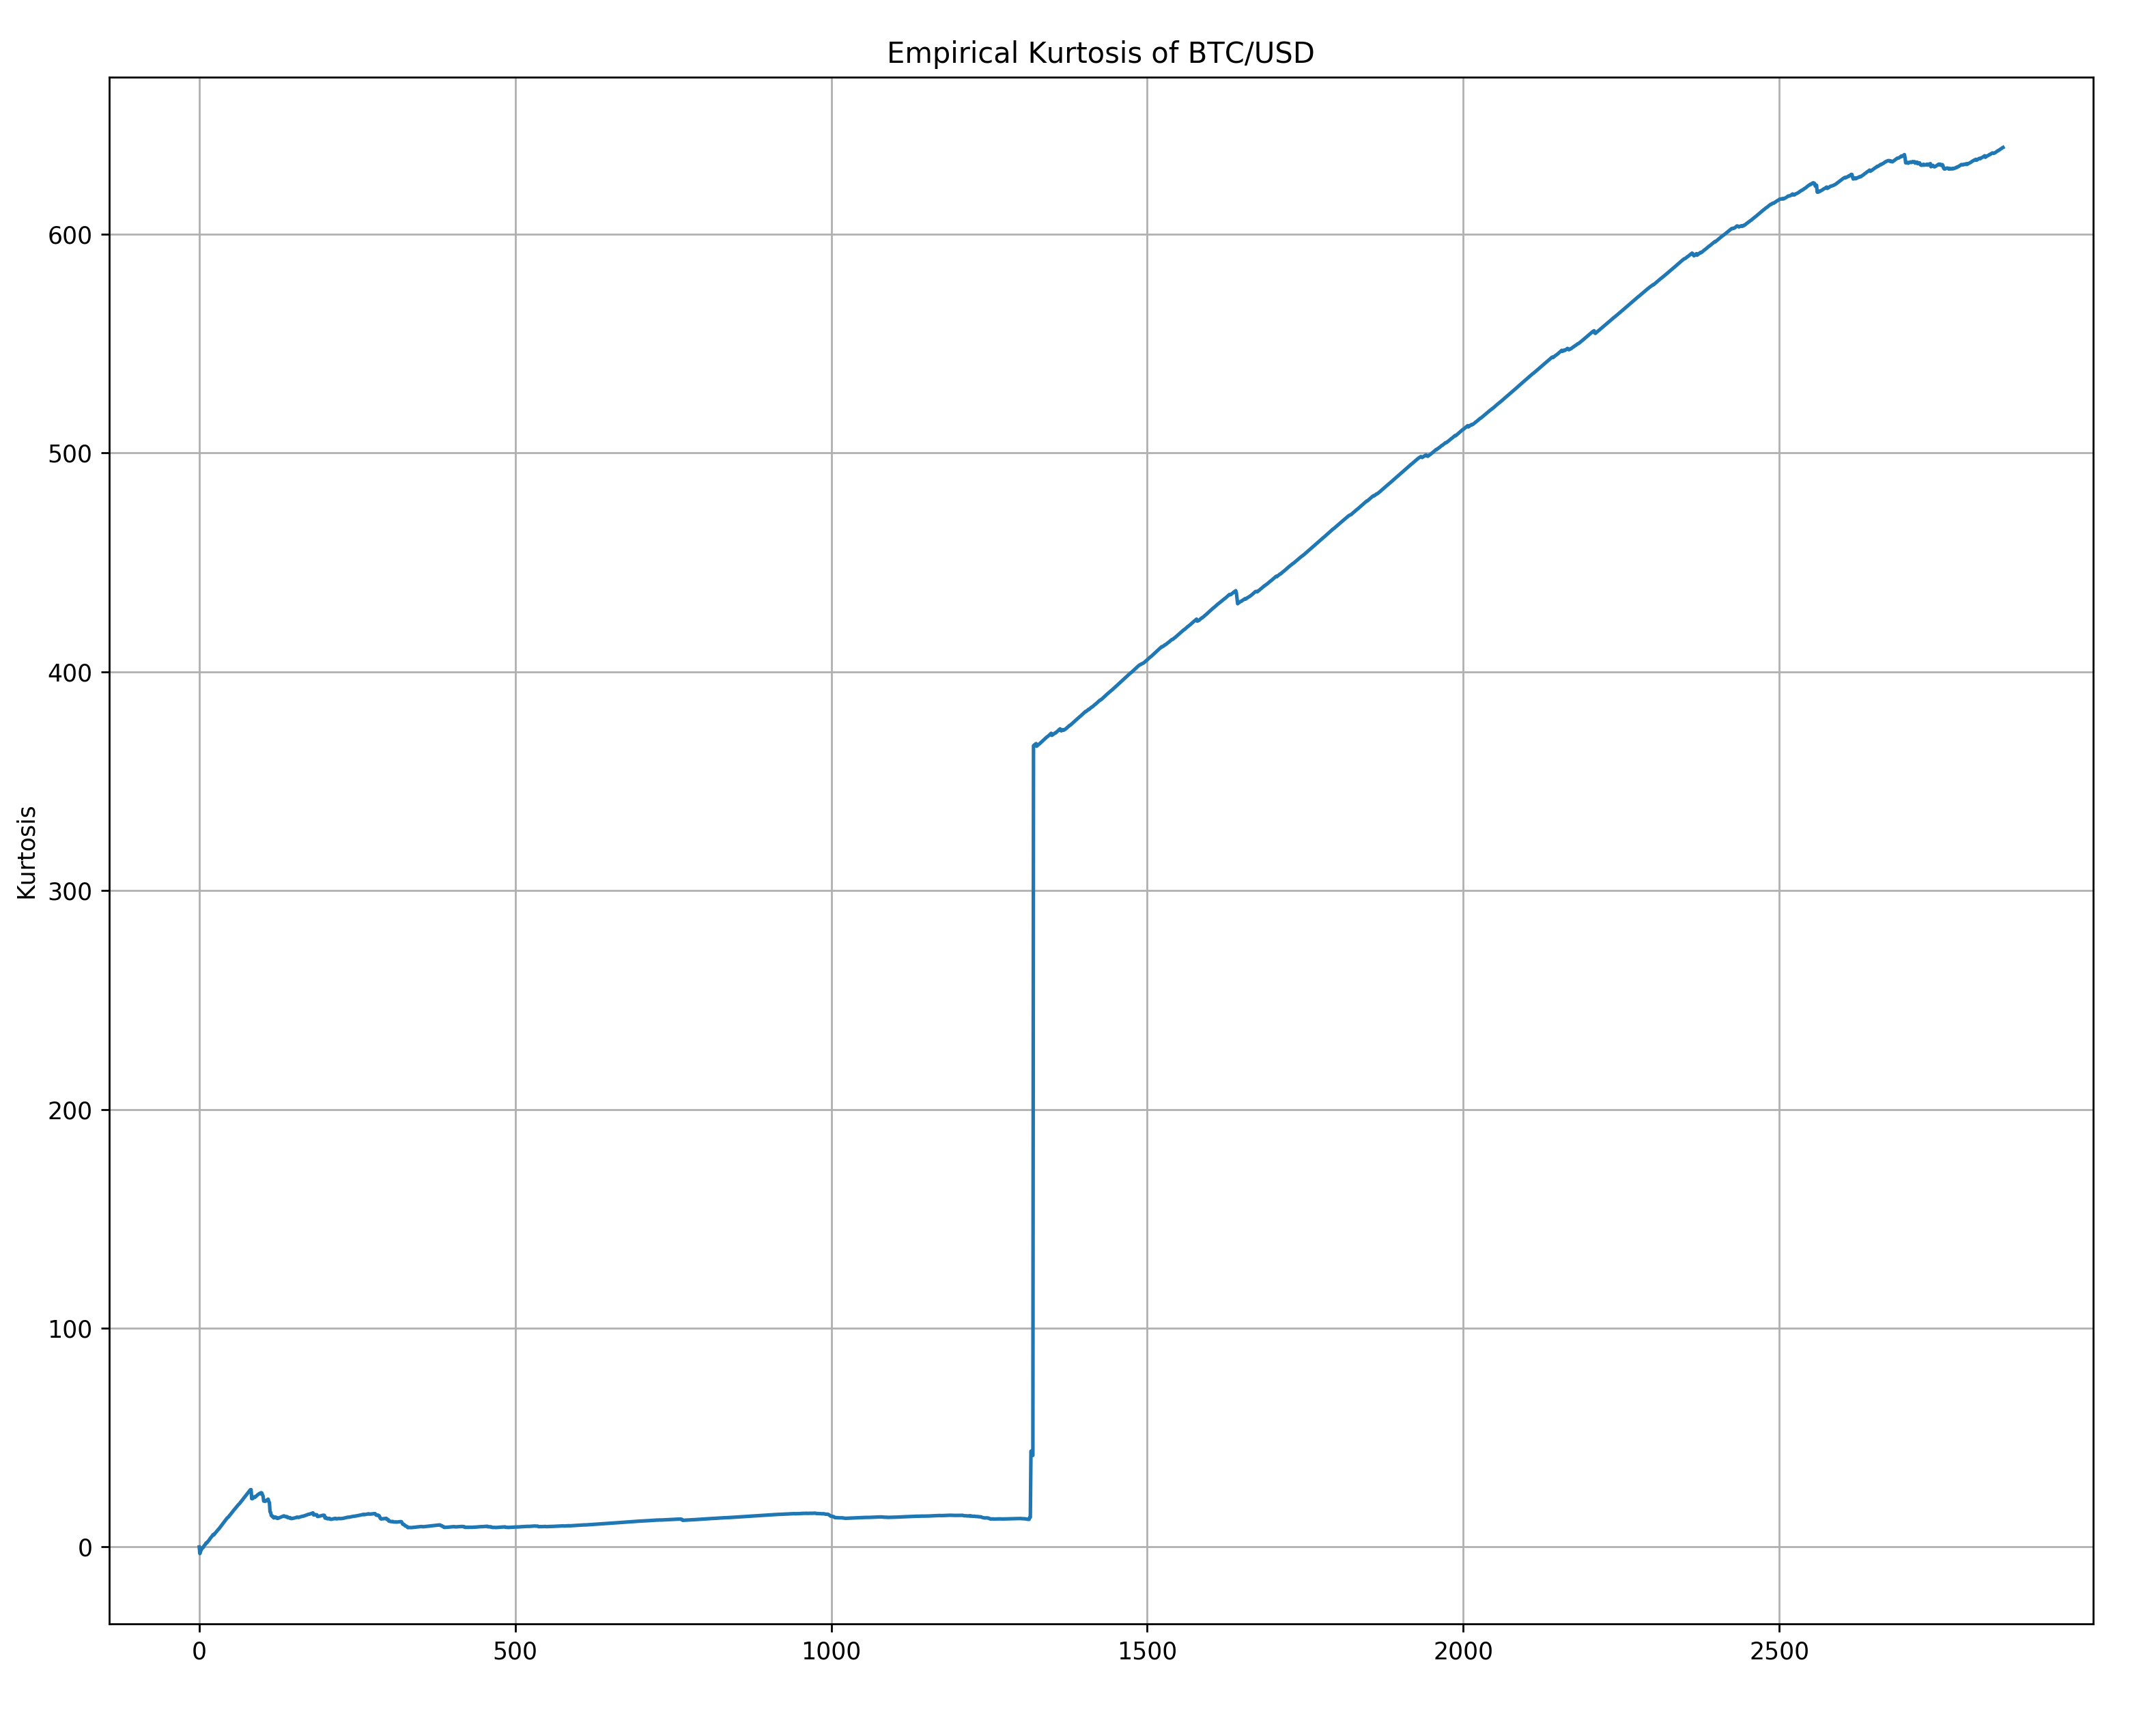
\includegraphics[width=\textwidth]{btc_returns_kurtosis.png}
\end{figure}
\end{frame}

%%%%%%%%%%%%%%%%%%%%%%%%%%%%%%%%%%%%%%%%%%%%%%%%%%%%%%%%%%%%%%%%%%%%%%%%%%%

\begin{frame}
\frametitle{GARCH(1,1) Prediction}

Recall the GARCH(1,1) model can be expressed as: $$X_t = \sigma_{t}\epsilon_{t}, \hspace{15pt} \epsilon_{t} \sim N(0,1)$$ where $\sigma_{t}^{2} = \a_0 + \beta_1 \sigma_{t-1}^{2} + \a_1 X_{t-1}^{2}$\\

\vspace{6pt}

To perform one-step ahead prediction with GARCH(1,1) we:
\begin{itemize}
\item{Estimate the parameters $\a_0, \beta_1$ and $\a_1$ using MLE}
\item{Let $a=\frac{\a_0}{1-\beta_1}$ and $a_i = \a_1\beta_1^{i-1}$ for $i=1,2,\dots$}
\end{itemize}
\vspace{6pt}
Then the $L_1$-optimal GARCH(1,1) predictor of $X_{n+1}^2$ is given by
$$ Median(X_{n+1}^2| \mathfrak{F_{n}}) = (a + \sum_{i=1}^{p} a_i X_{n+1-i}^2)Median(\epsilon_{n+1}^2) $$

%where we choose a very large choice for p to account for equivalence of GARCH(1,1) and ARCH($\infty$)

\end{frame}



\begin{frame}
\frametitle{Special Case: Uncorrelated NoVaS Series $W_{t,a}$}
\begin{figure}[h!]
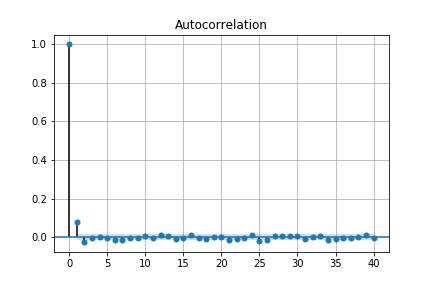
\includegraphics[width=\textwidth]{novas_sp500_returns_acf.png}
\end{figure}
\end{frame}


\begin{frame}
\frametitle{NoVaS Prediction in Special Case}
From the ACF plot on the previous slide, we can conclude that the NoVaS transformed series $\{W_{t,a}\}$ of the S\&P500 returns appears to be uncorrelated.\\

\vspace{5pt}

As a result we can predict $X_{n+1}^2$ (under $L_1$ loss) by

$$ X_{n+1}^2 = \widehat{\mu_2}A_{n}^2 $$

where

$$ \widehat{\mu_2} = median \{ \frac{W_{t,a}^2}{1-a_0W_{t,a}^2} ; t = p+1, p+2, \dots, n\} $$

and

$$ A_{n}^2 = \alpha s^2_{t-1} + \sum_{i=1}^{p} a_i X^2_{t+1-i} $$
\end{frame}


\begin{frame}
\frametitle{Bootstrap Prediction Intervals}
In addition to calculating point estimates, we calculate prediction intervals.\\
\vspace{5pt}
Below is an outline of the procedure used for NoVaS (GARCH is almost identical):

\begin{enumerate}
\item{Use Simple NoVaS to obtain transformation $\{W_{t,a}\}$ and fitted parameter $p$}
\item{Calculate $\widehat{g(X_{n+1})}$ the point predictor of $g(X_{n+1})$}
\item{Resample randomly (with replacement) the transformed variables  $\{W_{t,a}\}$ for $t=p+1,\dots,n$ to create the pseudo-data $W_{p+1}^*,\dots, W_{n-1}^*, W_{n}^*$ and $W_{n+1}^*$}
\item{Let $(X_{1}^*,\dots,X_{p}^*)' = (X_{1+I}^*,\dots,X_{p+I}^*)'$ where I $\sim \mathfrakk{U}\{0,n-p\}$}
\seti
\end{enumerate}

\end{frame}

\begin{frame}
\frametitle{Bootstrap Prediction Intervals}
\begin{enumerate}
\conti
\item{Generate the bootstrap pseudo-data $Y_{t}^*$ for $t=p+1,\dots,n$}
% using equation (10.17) $$ Y_{t}^* = \frac{W_{t}}{\sqrt{1-a_0W_{t}^{*2}}}\sqrt{\sum_{i=1}^{p} a_iY_{t-i}^{*2}}$$ for $t=p+1,\dots,n$}
\item{Based on the bootstrap data $Y_{1}^*,\dots,Y_{n}^*$ re-estimate the NoVaS transformation, then calculate the bootstrap predictor $\widehat{g(Y_{n+1}^*)}$}
\item{Calculate the bootstrap future value $Y_{n+1}^*$ and the bootstrap root: $g(Y_{n+1}^*) - \widehat{g(Y_{n+1}^*)}$}
\item{Repeat steps 3-7 B times - the B bootstrap root replicates are collected in the form of an empirical distribution whose $\alpha$-quantile is denoted $q(\alpha)$}
\item{The $(1-\alpha)100\%$ equal-tailed prediction interval for $g(Y_{n+1})$ is given by $$ [\widehat{g(Y_{n+1})} + q(\alpha/2), \widehat{g(Y_{n+1})} + q(1-\alpha/2)] $$}

\end{enumerate}
\end{frame}





\begin{frame}
\frametitle{S\&P500 Feb 2018 One Step Ahead Prediction}
Plot predicting S\&P500 Feb 2018 Volatility spike, along with prediction intervals

\end{frame}

\section{A Simple Volatility Trading Strategy}

\begin{frame}
\frametitle{Outline}
\tableofcontents[currentsection]
\end{frame}

\begin{frame}
\frametitle{Estimating the volatility $\mathbb{E}(X_{n+1}^2|\mathfrak{F_n})$
}

In order to implement our volatility trading strategy we'd ideally like an estimate of $\mathbb{E}(X_{n+1}^2|\mathfrak{F_{n}})$. \\

\vspace{5pt}

Fortunately, it is straightforward to do so under the case were the NoVaS series $W_{t,a}$ is uncorrelated and independent.

$$\mathbb{E}(X_{n+1}^2|\mathfrak{F_{n}}) = A_{n}^2 \mathbb{E} \bigg( \frac{W_{t,a}^2}{1-a_0 W_{t,a}^2} \bigg) $$

a natural estimate is therefore

$$ \frac{A_{n}^2}{n-p} \sum_{t=p+1}^{n} \bigg( \frac{W_{t,a}^2}{1-a_0 W_{t,a}^2} \bigg) $$

\end{frame}

\begin{frame}
\frametitle{Volatility Trading Strategy (Ahmad \& Wilmott 2005)}
\vspace{-2pt}
Relevant Definitions:
\begin{itemize}
\item{Implied Volatility (IV) - value calculated from an option price}
\vspace{2pt}
\item{VIX - popular index which is a measure of the stock market's expectation volatility implied by S\&P500 index options}
\vspace{2pt}
\item{VIX(t) = IV(t) current implied volatility}
\vspace{2pt}
\item{VXX - ETN that (imperfectly) tracks VIX index}
\vspace{2pt}
\item{RV(t+1) - is the GARCH or NoVaS predicted realized volatility for next period}
\vspace{2pt}
\item{Expect RV(t+1) to be better predictor of VIX(t+1) than VIX(t)}
\end{itemize}
\vspace{2pt}
Strategy:\\
\vspace{2pt}
\hspace{10pt}\textbf{If RV(t+1) - VIX(t) $>$ 0 then BUY VXX. Vice Versa}
\end{frame}

\begin{frame}
\frametitle{Strategy Results}
Cumulative returns plot, legend contains CAGR and Sharpe Ratio
\end{frame}

\end{document}